\chapter{Região de Desempenho Garantido}

\begin{equation}
  s = -\zeta\omega_n \pm \jmath\omega_n \sqrt {1-\zeta^2} \label{eq:PontoPlanoS}
\end{equation}

\begin{equation}
  z = \exp(sT_s)\label{eq:TransformacaoSZ}
\end{equation}

\begin{equation}
  z = \exp{\left(-\zeta\omega_nT_s \pm j\omega_nT_s\sqrt{1-\zeta^2}\right)}\label{eq:PontoPlanoZ}
\end{equation}

\begin{equation}
  z(\zeta,\omega_n) = \exp{\left(-\zeta\omega_nT_s \pm j\omega_nT_s\sqrt{1-\zeta^2}\right)}\label{eq:FuncaoPontoZ}
\end{equation}

\begin{equation}
  r = \exp{\left(-|\sigma|T_s\right)}\label{eq:RaioEstabilidadeRelativa}
\end{equation}

\begin{equation}
  \begin{bmatrix*}[c]
    -rP       & * \\
    PA + Z'B  & -rP
  \end{bmatrix*}
  \prec 0\label{eq:LMIEstabilidadeRelativa}
\end{equation}

\begin{equation}
  \begin{bmatrix*}[c]
    \sin{(\varphi)(AP + BZ + PA' + Z'B -2aP)} & * \\
    \cos{(\varphi)(PA' + Z'B'- AP - BZ)}      &  \sin{(\varphi)(AP + BZ + PA' + Z'B -2aP)}
  \end{bmatrix*}
  \prec 0\label{eq:LMIESetorConicoEsquerdo}
\end{equation}

\begin{equation}
  \begin{bmatrix*}[c]
    \sin{(\varphi)(2aP - AP - BZ - PA' - Z'B')} & * \\
    \cos{(\varphi)(PA' + Z'B' - AP - BZ)}       & \sin{(\varphi)(2aP - AP - BZ - PA' - Z'B')}
  \end{bmatrix*}
  \prec 0\label{eq:LMIESetorConicoDireito}
\end{equation}

\begin{equation}
  AP + BZ + Z'B' + PA' -2aP\label{eq:LMIRightBounded} \succ 0
\end{equation}

\begin{figure}
  \center
  % This file was created by matlab2tikz.
%
%The latest updates can be retrieved from
%  http://www.mathworks.com/matlabcentral/fileexchange/22022-matlab2tikz-matlab2tikz
%where you can also make suggestions and rate matlab2tikz.
%
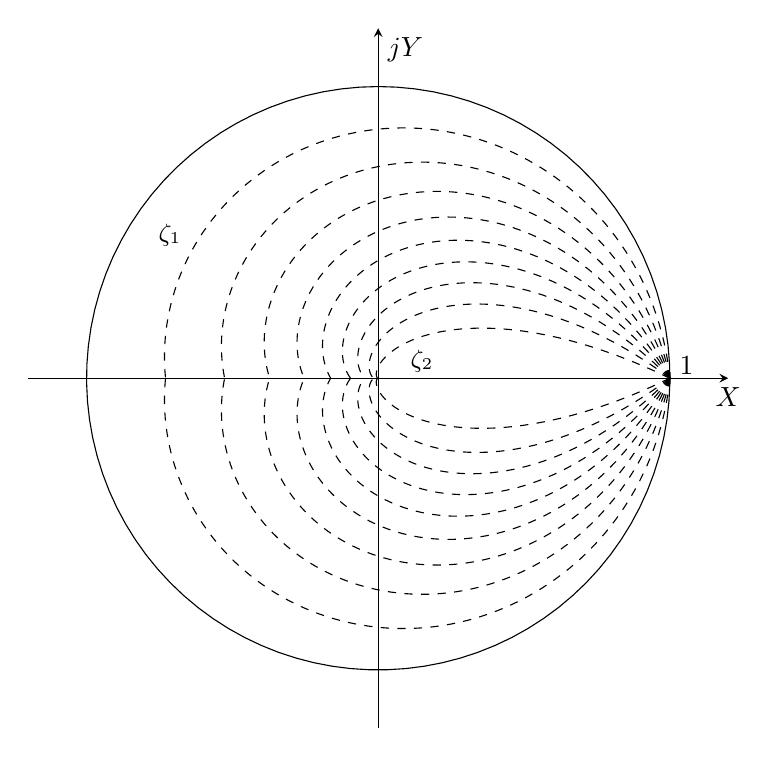
\begin{tikzpicture}

\begin{axis}[%
  axis lines=center,
  width=3.5in,
  height=3.5in,
  scale only axis,
  xmin=-1.2,
  xmax=1.2,
  ymin=-1.2,
  ymax=1.2,
  xtick={1},
  ytick=\empty,
  %xticklabels={},
  xticklabel style={anchor=south west},
  x label style={anchor=north},
  xlabel={$\pmb{X}$},
  ylabel={$\pmb{jY}$}
]
\addplot [color=black, forget plot]
  table[row sep=crcr]{%
0	1\\
0.0634239196565645	0.997986676471884\\
0.126592453573749	0.991954812830795\\
0.18925124436041	0.981928697262707\\
0.251147987181079	0.967948701396356\\
0.312033445698487	0.950071117740945\\
0.371662455660328	0.928367933016073\\
0.429794912089172	0.902926538286621\\
0.486196736100469	0.873849377069785\\
0.540640817455598	0.841253532831181\\
0.59290792905464	0.805270257531059\\
0.642787609686539	0.766044443118978\\
0.690079011482112	0.72373403810507\\
0.734591708657533	0.678509411557132\\
0.776146464291757	0.630552667084523\\
0.814575952050336	0.580056909571198\\
0.849725429949514	0.527225467610502\\
0.881453363447582	0.472271074772683\\
0.909631995354518	0.415415013001886\\
0.934147860265107	0.356886221591872\\
0.954902241444074	0.296920375328275\\
0.971811568323542	0.235758935509427\\
0.984807753012208	0.173648177666931\\
0.993838464461254	0.110838199901011\\
0.998867339183008	0.0475819158237424\\
0.999874127673875	-0.015865963834808\\
0.996854775951942	-0.0792499568567885\\
0.989821441880933	-0.142314838273285\\
0.978802446214779	-0.204806668065191\\
0.963842158559942	-0.266473813690035\\
0.945000818714669	-0.327067963317421\\
0.922354294104581	-0.386345125693128\\
0.895993774291336	-0.444066612605774\\
0.866025403784439	-0.5\\
0.832569854634771	-0.55392006386611\\
0.795761840530832	-0.605609687137666\\
0.755749574354258	-0.654860733945285\\
0.712694171378863	-0.701474887706321\\
0.666769000516292	-0.745264449675755\\
0.618158986220605	-0.786053094742787\\
0.567059863862771	-0.823676581429833\\
0.513677391573407	-0.857983413234977\\
0.458226521727411	-0.888835448654923\\
0.400930535406614	-0.916108457432069\\
0.342020143325669	-0.939692620785908\\
0.28173255684143	-0.959492973614497\\
0.220310532786541	-0.975429786885407\\
0.15800139597335	-0.987438888676394\\
0.0950560433041829	-0.995471922573085\\
0.0317279334980681	-0.999496542383185\\
-0.0317279334980679	-0.999496542383185\\
-0.0950560433041826	-0.995471922573085\\
-0.15800139597335	-0.987438888676394\\
-0.220310532786541	-0.975429786885407\\
-0.281732556841429	-0.959492973614497\\
-0.342020143325669	-0.939692620785908\\
-0.400930535406613	-0.91610845743207\\
-0.45822652172741	-0.888835448654924\\
-0.513677391573406	-0.857983413234977\\
-0.567059863862771	-0.823676581429833\\
-0.618158986220605	-0.786053094742788\\
-0.666769000516292	-0.745264449675755\\
-0.712694171378863	-0.701474887706322\\
-0.755749574354258	-0.654860733945285\\
-0.795761840530832	-0.605609687137667\\
-0.832569854634771	-0.55392006386611\\
-0.866025403784438	-0.5\\
-0.895993774291336	-0.444066612605774\\
-0.922354294104581	-0.386345125693129\\
-0.945000818714668	-0.327067963317422\\
-0.963842158559942	-0.266473813690035\\
-0.978802446214779	-0.204806668065191\\
-0.989821441880933	-0.142314838273285\\
-0.996854775951942	-0.0792499568567888\\
-0.999874127673875	-0.0158659638348076\\
-0.998867339183008	0.0475819158237424\\
-0.993838464461254	0.110838199901011\\
-0.984807753012208	0.17364817766693\\
-0.971811568323542	0.235758935509427\\
-0.954902241444074	0.296920375328275\\
-0.934147860265107	0.356886221591872\\
-0.909631995354519	0.415415013001886\\
-0.881453363447582	0.472271074772682\\
-0.849725429949514	0.527225467610502\\
-0.814575952050336	0.580056909571198\\
-0.776146464291757	0.630552667084522\\
-0.734591708657534	0.678509411557132\\
-0.690079011482113	0.723734038105069\\
-0.64278760968654	0.766044443118977\\
-0.59290792905464	0.805270257531059\\
-0.540640817455597	0.841253532831181\\
-0.486196736100469	0.873849377069785\\
-0.429794912089172	0.902926538286621\\
-0.371662455660328	0.928367933016072\\
-0.312033445698487	0.950071117740945\\
-0.251147987181079	0.967948701396356\\
-0.189251244360411	0.981928697262707\\
-0.12659245357375	0.991954812830795\\
-0.0634239196565654	0.997986676471884\\
-2.44929359829471e-16	1\\
};
\addplot [color=black, dashed, forget plot]
  table[row sep=crcr]{%
1	0\\
0.996355675894196	0.031311738544454\\
0.991744207915904	0.0623952568417635\\
0.986176266623562	0.0932211036444067\\
0.979663405858395	0.123760269148488\\
0.972218045703082	0.153984211042097\\
0.963853454686905	0.183864879925138\\
0.954583731259804	0.213374744079341\\
0.944423784558363	0.242486813567919\\
0.933389314487286	0.271174663645149\\
0.921496791140463	0.299412457456957\\
0.908763433586244	0.327174968014412\\
0.895207188041996	0.354437599422875\\
0.880846705463472	0.381176407350381\\
0.865701318574964	0.407368118719727\\
0.849791018366557	0.432990150609548\\
0.833136430085219	0.458020628350625\\
0.815758788746754	0.48243840280446\\
0.797679914195986	0.506223066812133\\
0.778922185742773	0.529354970802303\\
0.759508516401756	0.551815237548133\\
0.739462326763917	0.573585776063844\\
0.718807518528229	0.594649294632494\\
0.697568447721846	0.614989312957509\\
0.675769897637407	0.634590173431413\\
0.653437051516106	0.653437051516106\\
0.630595465005309	0.671515965229972\\
0.607271038419472	0.688813783738016\\
0.583489988833183	0.70531823504214\\
0.559278822035108	0.721017912769564\\
0.534664304371591	0.735902282058355\\
0.509673434508578	0.749961684539869\\
0.48433341514044	0.763187342418857\\
0.458671624674142	0.775571361652856\\
0.432715588917053	0.78710673423337\\
0.406492952796512	0.797787339572243\\
0.380031452139034	0.807607944997462\\
0.353358885536856	0.816564205363516\\
0.326503086329192	0.824652661782262\\
0.299491894725349	0.831870739481111\\
0.272353130096494	0.83821674479613\\
0.245114563462553	0.843689861308526\\
0.217803890200343	0.848290145133715\\
0.190448702998685	0.852018519373006\\
0.163076465085787	0.854876767738689\\
0.135714483753824	0.856867527364047\\
0.108389884205117	0.857994280810589\\
0.0811295837439053	0.858261347285484\\
0.0539602663371597	0.857673873082901\\
0.0269083575674107	0.856237821263645\\
5.22899666167123e-17	0.853959960588124\\
-0.0267389710133675	0.850847853718362\\
-0.0532830510734783	0.846909844705366\\
-0.0796070899941588	0.8421550457788\\
-0.105686314564419	0.836593323456462\\
-0.131496350792703	0.830235283991667\\
-0.157013245614411	0.823092258177157\\
-0.182213488044495	0.815176285524687\\
-0.2070740297576	0.806500097839947\\
-0.23157230507891	0.797077102212939\\
-0.255686250369537	0.786921363444393\\
-0.279394322791008	0.776047585929238\\
-0.302675518434107	0.764471095018548\\
-0.325509389798054	0.752207817881766\\
-0.347876062606756	0.739274263891364\\
-0.369756251949576	0.725687504552447\\
-0.391131277734848	0.711465153000104\\
-0.411983079445094	0.696625343087594\\
-0.432294230183688	0.681186708088743\\
-0.452047950003462	0.665168359038114\\
-0.47122811850853	0.648589862732789\\
-0.489819286721389	0.631471219419718\\
-0.507806688208121	0.613832840192814\\
-0.525176249455312	0.595695524124067\\
-0.541914599493101	0.577080435153081\\
-0.558009078759514	0.558009078759514\\
-0.573447747202083	0.538503278442984\\
-0.588219391613473	0.518585152035002\\
-0.602313532198671	0.49827708786755\\
-0.615720428372028	0.477601720822873\\
-0.628431083783263	0.456581908289041\\
-0.64043725057227	0.43524070604576\\
-0.651731432853363	0.413601344104843\\
-0.662306889430351	0.391687202529621\\
-0.672157635744576	0.369521787257474\\
-0.681278445058817	0.347128705949459\\
-0.689664848880689	0.324531643890898\\
-0.697313136629901	0.301754339966517\\
-0.704220354554473	0.278820562733578\\
-0.710384303901703	0.255754086616121\\
-0.715803538350409	0.232578668243255\\
-0.720477360711629	0.209318022954057\\
-0.724405818905681	0.185995801491425\\
-0.727589701224124	0.162635566906816\\
-0.730030530885834	0.139260771697509\\
-0.731730559897045	0.115894735197653\\
-0.732692762225847	0.0925606212439533\\
-0.732920826302222	0.0692814161364764\\
-0.732419146855338	0.0460799069146058\\
-0.731192816100364	0.0229786599677571\\
-0.729247614287671	8.9307075662324e-17\\
};
\addplot [color=black, dashed, forget plot]
  table[row sep=crcr]{%
1	-0\\
0.996355675894196	-0.031311738544454\\
0.991744207915904	-0.0623952568417635\\
0.986176266623562	-0.0932211036444067\\
0.979663405858395	-0.123760269148488\\
0.972218045703082	-0.153984211042097\\
0.963853454686905	-0.183864879925138\\
0.954583731259804	-0.213374744079341\\
0.944423784558363	-0.242486813567919\\
0.933389314487286	-0.271174663645149\\
0.921496791140463	-0.299412457456957\\
0.908763433586244	-0.327174968014412\\
0.895207188041996	-0.354437599422875\\
0.880846705463472	-0.381176407350381\\
0.865701318574964	-0.407368118719727\\
0.849791018366557	-0.432990150609548\\
0.833136430085219	-0.458020628350625\\
0.815758788746754	-0.48243840280446\\
0.797679914195986	-0.506223066812133\\
0.778922185742773	-0.529354970802303\\
0.759508516401756	-0.551815237548133\\
0.739462326763917	-0.573585776063844\\
0.718807518528229	-0.594649294632494\\
0.697568447721846	-0.614989312957509\\
0.675769897637407	-0.634590173431413\\
0.653437051516106	-0.653437051516106\\
0.630595465005309	-0.671515965229972\\
0.607271038419472	-0.688813783738016\\
0.583489988833183	-0.70531823504214\\
0.559278822035108	-0.721017912769564\\
0.534664304371591	-0.735902282058355\\
0.509673434508578	-0.749961684539869\\
0.48433341514044	-0.763187342418857\\
0.458671624674142	-0.775571361652856\\
0.432715588917053	-0.78710673423337\\
0.406492952796512	-0.797787339572243\\
0.380031452139034	-0.807607944997462\\
0.353358885536856	-0.816564205363516\\
0.326503086329192	-0.824652661782262\\
0.299491894725349	-0.831870739481111\\
0.272353130096494	-0.83821674479613\\
0.245114563462553	-0.843689861308526\\
0.217803890200343	-0.848290145133715\\
0.190448702998685	-0.852018519373006\\
0.163076465085787	-0.854876767738689\\
0.135714483753824	-0.856867527364047\\
0.108389884205117	-0.857994280810589\\
0.0811295837439053	-0.858261347285484\\
0.0539602663371597	-0.857673873082901\\
0.0269083575674107	-0.856237821263645\\
5.22899666167123e-17	-0.853959960588124\\
-0.0267389710133675	-0.850847853718362\\
-0.0532830510734783	-0.846909844705366\\
-0.0796070899941588	-0.8421550457788\\
-0.105686314564419	-0.836593323456462\\
-0.131496350792703	-0.830235283991667\\
-0.157013245614411	-0.823092258177157\\
-0.182213488044495	-0.815176285524687\\
-0.2070740297576	-0.806500097839947\\
-0.23157230507891	-0.797077102212939\\
-0.255686250369537	-0.786921363444393\\
-0.279394322791008	-0.776047585929238\\
-0.302675518434107	-0.764471095018548\\
-0.325509389798054	-0.752207817881766\\
-0.347876062606756	-0.739274263891364\\
-0.369756251949576	-0.725687504552447\\
-0.391131277734848	-0.711465153000104\\
-0.411983079445094	-0.696625343087594\\
-0.432294230183688	-0.681186708088743\\
-0.452047950003462	-0.665168359038114\\
-0.47122811850853	-0.648589862732789\\
-0.489819286721389	-0.631471219419718\\
-0.507806688208121	-0.613832840192814\\
-0.525176249455312	-0.595695524124067\\
-0.541914599493101	-0.577080435153081\\
-0.558009078759514	-0.558009078759514\\
-0.573447747202083	-0.538503278442984\\
-0.588219391613473	-0.518585152035002\\
-0.602313532198671	-0.49827708786755\\
-0.615720428372028	-0.477601720822873\\
-0.628431083783263	-0.456581908289041\\
-0.64043725057227	-0.43524070604576\\
-0.651731432853363	-0.413601344104843\\
-0.662306889430351	-0.391687202529621\\
-0.672157635744576	-0.369521787257474\\
-0.681278445058817	-0.347128705949459\\
-0.689664848880689	-0.324531643890898\\
-0.697313136629901	-0.301754339966517\\
-0.704220354554473	-0.278820562733578\\
-0.710384303901703	-0.255754086616121\\
-0.715803538350409	-0.232578668243255\\
-0.720477360711629	-0.209318022954057\\
-0.724405818905681	-0.185995801491425\\
-0.727589701224124	-0.162635566906816\\
-0.730030530885834	-0.139260771697509\\
-0.731730559897045	-0.115894735197653\\
-0.732692762225847	-0.0925606212439533\\
-0.732920826302222	-0.0692814161364764\\
-0.732419146855338	-0.0460799069146058\\
-0.731192816100364	-0.0229786599677571\\
-0.729247614287671	-8.9307075662324e-17\\
};
\addplot [color=black, dashed, forget plot]
  table[row sep=crcr]{%
1	0\\
0.993117483189145	0.0312099742390054\\
0.985308272923941	0.0619903421332781\\
0.97659215519062	0.0923151383768702\\
0.966989590174559	0.122159193890609\\
0.956521682769877	0.151498151383791\\
0.94521015280632	0.180308479888376\\
0.933077305027449	0.208567488263936\\
0.920145998853958	0.236253337672669\\
0.906439617965761	0.263345053024872\\
0.891982039736211	0.289822533396298\\
0.876797604551564	0.315666561419856\\
0.86091108504849	0.340858811655134\\
0.844347655302098	0.365381857940227\\
0.82713285999656	0.389219179731315\\
0.809292583610081	0.412355167436434\\
0.790853019645473	0.434775126750799\\
0.771840639937194	0.456465282001969\\
0.752282164065243	0.477412778514076\\
0.732204528905761	0.497605684001175\\
0.711634858347723	0.517032989000692\\
0.690600433204527	0.535684606358738\\
0.669128661348724	0.553551369779917\\
0.647247048097569	0.570625031455008\\
0.624983166876419	0.586898258780722\\
0.602364630186426	0.602364630186426\\
0.579419060902297	0.61701863008351\\
0.556174063925214	0.630855642953699\\
0.532657198215371	0.643871946593355\\
0.508895949227834	0.656064704531411\\
0.484917701774751	0.667431957639199\\
0.460749713336196	0.677972614951073\\
0.436419087841189	0.687686443715224\\
0.411952749939678	0.696574058694691\\
0.38737741978552	0.704636910739023\\
0.362719588349683	0.711877274647591\\
0.338005493282155	0.718298236345939\\
0.313261095340199	0.723903679397059\\
0.28851205539983	0.728698270869819\\
0.263783712066551	0.732687446587187\\
0.239101059900595	0.735877395777214\\
0.214488728271062	0.738275045150065\\
0.189970960852564	0.739888042424682\\
0.165571595777099	0.74072473932891\\
0.141314046453114	0.740794174097177\\
0.117221283062812	0.740106053489981\\
0.093315814747988	0.738670734359673\\
0.0696196724937937	0.736499204787132\\
0.0461543927190345	0.733603064814063\\
0.0229410015807486	0.729994506795762\\
4.44354699422903e-17	0.725686295399261\\
-0.0226486505850102	0.720691747271768\\
-0.0449855417332313	0.715024710404419\\
-0.0669918307779809	0.708699543216261\\
-0.0886492528634361	0.701731093383425\\
-0.109940132237539	0.694134676438339\\
-0.130847392799268	0.685926054163788\\
-0.151354567898984	0.677121412806495\\
-0.17144580939139	0.667737341134781\\
-0.191105895941341	0.657790808364695\\
-0.210320240583588	0.647299141978847\\
-0.229074897538198	0.63628000546197\\
-0.247356568284209	0.624751375976997\\
-0.265152606894742	0.612731522005231\\
-0.282451024637557	0.600238980973899\\
-0.299240493845688	0.587292536894097\\
-0.315510351063531	0.573911198031842\\
-0.331250599474388	0.560114174634617\\
-0.346451910616147	0.545920856735445\\
-0.361105625392428	0.531350792056182\\
-0.375203754387119	0.516423664031337\\
-0.388738977490884	0.501159269973318\\
-0.401704642848774	0.485577499399622\\
-0.414094765138671	0.469698312542032\\
-0.425904023190858	0.453541719057446\\
-0.437127756959533	0.437127756959533\\
-0.447761963857629	0.420476471789907\\
-0.457803294466788	0.40360789604704\\
-0.467249047634843	0.386542028890662\\
-0.47609716497361	0.369298816138837\\
-0.484346224770267	0.351898130574443\\
-0.491995435325994	0.334359752577216\\
-0.499044627735993	0.316703351096997\\
-0.505494248125377	0.298948464983263\\
-0.511345349355781	0.281114484685478\\
-0.516599582217932	0.263220634338226\\
-0.521259186125707	0.245285954244527\\
-0.525326979327546	0.227329283770144\\
-0.528806348651366	0.209369244661129\\
-0.531701238799399	0.191424224796241\\
-0.534016141209622	0.173512362385299\\
-0.535756082500673	0.155651530623926\\
-0.536926612517378	0.137859322814535\\
-0.53753379199418	0.120153037962827\\
-0.537584179853935	0.102549666858439\\
-0.537084820159711	0.0850658786478001\\
-0.536043228737323	0.0677180079066311\\
-0.534467379486475	0.0505220422189308\\
-0.532365690398461	0.0334936102686788\\
-0.529747009298427	0.016647970449882\\
-0.526620599330303	6.44924231334916e-17\\
};
\addplot [color=black, dashed, forget plot]
  table[row sep=crcr]{%
1	-0\\
0.993117483189145	-0.0312099742390054\\
0.985308272923941	-0.0619903421332781\\
0.97659215519062	-0.0923151383768702\\
0.966989590174559	-0.122159193890609\\
0.956521682769877	-0.151498151383791\\
0.94521015280632	-0.180308479888376\\
0.933077305027449	-0.208567488263936\\
0.920145998853958	-0.236253337672669\\
0.906439617965761	-0.263345053024872\\
0.891982039736211	-0.289822533396298\\
0.876797604551564	-0.315666561419856\\
0.86091108504849	-0.340858811655134\\
0.844347655302098	-0.365381857940227\\
0.82713285999656	-0.389219179731315\\
0.809292583610081	-0.412355167436434\\
0.790853019645473	-0.434775126750799\\
0.771840639937194	-0.456465282001969\\
0.752282164065243	-0.477412778514076\\
0.732204528905761	-0.497605684001175\\
0.711634858347723	-0.517032989000692\\
0.690600433204527	-0.535684606358738\\
0.669128661348724	-0.553551369779917\\
0.647247048097569	-0.570625031455008\\
0.624983166876419	-0.586898258780722\\
0.602364630186426	-0.602364630186426\\
0.579419060902297	-0.61701863008351\\
0.556174063925214	-0.630855642953699\\
0.532657198215371	-0.643871946593355\\
0.508895949227834	-0.656064704531411\\
0.484917701774751	-0.667431957639199\\
0.460749713336196	-0.677972614951073\\
0.436419087841189	-0.687686443715224\\
0.411952749939678	-0.696574058694691\\
0.38737741978552	-0.704636910739023\\
0.362719588349683	-0.711877274647591\\
0.338005493282155	-0.718298236345939\\
0.313261095340199	-0.723903679397059\\
0.28851205539983	-0.728698270869819\\
0.263783712066551	-0.732687446587187\\
0.239101059900595	-0.735877395777214\\
0.214488728271062	-0.738275045150065\\
0.189970960852564	-0.739888042424682\\
0.165571595777099	-0.74072473932891\\
0.141314046453114	-0.740794174097177\\
0.117221283062812	-0.740106053489981\\
0.093315814747988	-0.738670734359673\\
0.0696196724937937	-0.736499204787132\\
0.0461543927190345	-0.733603064814063\\
0.0229410015807486	-0.729994506795762\\
4.44354699422903e-17	-0.725686295399261\\
-0.0226486505850102	-0.720691747271768\\
-0.0449855417332313	-0.715024710404419\\
-0.0669918307779809	-0.708699543216261\\
-0.0886492528634361	-0.701731093383425\\
-0.109940132237539	-0.694134676438339\\
-0.130847392799268	-0.685926054163788\\
-0.151354567898984	-0.677121412806495\\
-0.17144580939139	-0.667737341134781\\
-0.191105895941341	-0.657790808364695\\
-0.210320240583588	-0.647299141978847\\
-0.229074897538198	-0.63628000546197\\
-0.247356568284209	-0.624751375976997\\
-0.265152606894742	-0.612731522005231\\
-0.282451024637557	-0.600238980973899\\
-0.299240493845688	-0.587292536894097\\
-0.315510351063531	-0.573911198031842\\
-0.331250599474388	-0.560114174634617\\
-0.346451910616147	-0.545920856735445\\
-0.361105625392428	-0.531350792056182\\
-0.375203754387119	-0.516423664031337\\
-0.388738977490884	-0.501159269973318\\
-0.401704642848774	-0.485577499399622\\
-0.414094765138671	-0.469698312542032\\
-0.425904023190858	-0.453541719057446\\
-0.437127756959533	-0.437127756959533\\
-0.447761963857629	-0.420476471789907\\
-0.457803294466788	-0.40360789604704\\
-0.467249047634843	-0.386542028890662\\
-0.47609716497361	-0.369298816138837\\
-0.484346224770267	-0.351898130574443\\
-0.491995435325994	-0.334359752577216\\
-0.499044627735993	-0.316703351096997\\
-0.505494248125377	-0.298948464983263\\
-0.511345349355781	-0.281114484685478\\
-0.516599582217932	-0.263220634338226\\
-0.521259186125707	-0.245285954244527\\
-0.525326979327546	-0.227329283770144\\
-0.528806348651366	-0.209369244661129\\
-0.531701238799399	-0.191424224796241\\
-0.534016141209622	-0.173512362385299\\
-0.535756082500673	-0.155651530623926\\
-0.536926612517378	-0.137859322814535\\
-0.53753379199418	-0.120153037962827\\
-0.537584179853935	-0.102549666858439\\
-0.537084820159711	-0.0850658786478001\\
-0.536043228737323	-0.0677180079066311\\
-0.534467379486475	-0.0505220422189308\\
-0.532365690398461	-0.0334936102686788\\
-0.529747009298427	-0.016647970449882\\
-0.526620599330303	-6.44924231334916e-17\\
};
\addplot [color=black, dashed, forget plot]
  table[row sep=crcr]{%
1	0\\
0.989680205048008	0.031101953421677\\
0.978499576757223	0.0615619752795178\\
0.966486964076787	0.0913599165772274\\
0.953671544913749	0.120476733510694\\
0.940082788364644	0.148894486293864\\
0.925750417373368	0.176596336822066\\
0.910704371847075	0.203566545198034\\
0.894974772260769	0.22979046514661\\
0.878591883780097	0.255254538344805\\
0.86158608093073	0.279946287694513\\
0.843987812841589	0.303854309565807\\
0.825827569087992	0.326968265039271\\
0.807135846159684	0.349278870176369\\
0.787943114577512	0.37077788534731\\
0.768279786681378	0.391458103646313\\
0.748176185110921	0.411313338424568\\
0.727662511999217	0.430338409971535\\
0.70676881889864	0.448529131375562\\
0.685524977456837	0.465882293595051\\
0.663960650859636	0.482395649771645\\
0.642105266056556	0.498067898817131\\
0.619987986783415	0.512898668305873\\
0.597637687395423	0.526888496704744\\
0.575082927522991	0.540038814972599\\
0.552351927561387	0.552351927561387\\
0.529472545004228	0.563830992851004\\
0.506472251629725	0.574480003049982\\
0.483378111547487	0.584303763594046\\
0.460216760112624	0.593307872074486\\
0.437014383712816	0.601498696728173\\
0.41379670043299	0.608883354520886\\
0.390588941601167	0.61546968885546\\
0.367415834218091	0.621266246936007\\
0.344301584272182	0.626282256819272\\
0.321269860940431	0.630527604183869\\
0.298343781674863	0.634012808847879\\
0.275545898173243	0.636749001064931\\
0.252898183231812	0.638747897628573\\
0.23042201847689	0.640021777814333\\
0.208138182971344	0.640583459188477\\
0.186066842691023	0.640446273312061\\
0.164227540865449	0.639624041368408\\
0.142639189176222	0.638131049741675\\
0.121320059805814	0.635982025573706\\
0.100287778328637	0.633192112325829\\
0.0795593174355637	0.629776845371748\\
0.0591509914823055	0.625752127647141\\
0.0390784518514043	0.621134205380978\\
0.019356683116887	0.615939643933052\\
3.73630739569175e-17	0.610185303761559\\
-0.0189779548961836	0.603888316544021\\
-0.0375642125860939	0.597066061474163\\
-0.055746478448306	0.589736141756782\\
-0.0735131322334228	0.581916361321951\\
-0.0908532273476422	0.573624701779294\\
-0.107756489426951	0.564879299632359\\
-0.124213314217353	0.555698423772488\\
-0.140214764776994	0.54610045327087\\
-0.155752568016441	0.536103855486799\\
-0.170819110593797	0.525727164509449\\
-0.185407434181671	0.514988959949799\\
-0.199511230123377	0.503907846098627\\
-0.213124833496062	0.49250243146579\\
-0.226243216598717	0.480791308715308\\
-0.23886198188335	0.468793035010043\\
-0.250977354347776	0.456526112779072\\
-0.262586173408747	0.444008970920142\\
-0.273685884274306	0.431259946448866\\
-0.284274528834428	0.418297266605636\\
-0.294350736089166	0.40513903143051\\
-0.303913712133613	0.391803196815617\\
-0.312963229719119	0.378307558043956\\
-0.321499617410256	0.364669733822732\\
-0.329523748357088	0.350907150818703\\
-0.337037028702328	0.337037028702328\\
-0.344041385642971	0.323076365706811\\
-0.350539255165994	0.309041924707485\\
-0.356533569477655	0.294950219826293\\
-0.362027744145895	0.280817503565482\\
-0.367025664975262	0.266659754473976\\
-0.371531674633684	0.252492665349235\\
-0.375550559050301	0.238331631976814\\
-0.379087533603451	0.224191742409173\\
-0.382148229117742	0.210087766784708\\
-0.384738677688982	0.196034147687371\\
-0.386865298355562	0.182044991046649\\
-0.388534882634674	0.168134057577092\\
-0.389754579941548	0.15431475475605\\
-0.390531882909652	0.140600129337673\\
-0.390874612629551	0.127002860400749\\
-0.390790903823879	0.113535252927376\\
-0.390289189975578	0.100209231908998\\
-0.389378188426307	0.0870363369757959\\
-0.388066885461584	0.0740277175449813\\
-0.386364521398959	0.0611941284830315\\
-0.384280575695157	0.0485459262764819\\
-0.381824752087813	0.0360930657054282\\
-0.379006963787087	0.0238450970134807\\
-0.375837318732076	0.0118111635674941\\
-0.372326104926586	4.55967972637346e-17\\
};
\addplot [color=black, dashed, forget plot]
  table[row sep=crcr]{%
1	-0\\
0.989680205048008	-0.031101953421677\\
0.978499576757223	-0.0615619752795178\\
0.966486964076787	-0.0913599165772274\\
0.953671544913749	-0.120476733510694\\
0.940082788364644	-0.148894486293864\\
0.925750417373368	-0.176596336822066\\
0.910704371847075	-0.203566545198034\\
0.894974772260769	-0.22979046514661\\
0.878591883780097	-0.255254538344805\\
0.86158608093073	-0.279946287694513\\
0.843987812841589	-0.303854309565807\\
0.825827569087992	-0.326968265039271\\
0.807135846159684	-0.349278870176369\\
0.787943114577512	-0.37077788534731\\
0.768279786681378	-0.391458103646313\\
0.748176185110921	-0.411313338424568\\
0.727662511999217	-0.430338409971535\\
0.70676881889864	-0.448529131375562\\
0.685524977456837	-0.465882293595051\\
0.663960650859636	-0.482395649771645\\
0.642105266056556	-0.498067898817131\\
0.619987986783415	-0.512898668305873\\
0.597637687395423	-0.526888496704744\\
0.575082927522991	-0.540038814972599\\
0.552351927561387	-0.552351927561387\\
0.529472545004228	-0.563830992851004\\
0.506472251629725	-0.574480003049982\\
0.483378111547487	-0.584303763594046\\
0.460216760112624	-0.593307872074486\\
0.437014383712816	-0.601498696728173\\
0.41379670043299	-0.608883354520886\\
0.390588941601167	-0.61546968885546\\
0.367415834218091	-0.621266246936007\\
0.344301584272182	-0.626282256819272\\
0.321269860940431	-0.630527604183869\\
0.298343781674863	-0.634012808847879\\
0.275545898173243	-0.636749001064931\\
0.252898183231812	-0.638747897628573\\
0.23042201847689	-0.640021777814333\\
0.208138182971344	-0.640583459188477\\
0.186066842691023	-0.640446273312061\\
0.164227540865449	-0.639624041368408\\
0.142639189176222	-0.638131049741675\\
0.121320059805814	-0.635982025573706\\
0.100287778328637	-0.633192112325829\\
0.0795593174355637	-0.629776845371748\\
0.0591509914823055	-0.625752127647141\\
0.0390784518514043	-0.621134205380978\\
0.019356683116887	-0.615939643933052\\
3.73630739569175e-17	-0.610185303761559\\
-0.0189779548961836	-0.603888316544021\\
-0.0375642125860939	-0.597066061474163\\
-0.055746478448306	-0.589736141756782\\
-0.0735131322334228	-0.581916361321951\\
-0.0908532273476422	-0.573624701779294\\
-0.107756489426951	-0.564879299632359\\
-0.124213314217353	-0.555698423772488\\
-0.140214764776994	-0.54610045327087\\
-0.155752568016441	-0.536103855486799\\
-0.170819110593797	-0.525727164509449\\
-0.185407434181671	-0.514988959949799\\
-0.199511230123377	-0.503907846098627\\
-0.213124833496062	-0.49250243146579\\
-0.226243216598717	-0.480791308715308\\
-0.23886198188335	-0.468793035010043\\
-0.250977354347776	-0.456526112779072\\
-0.262586173408747	-0.444008970920142\\
-0.273685884274306	-0.431259946448866\\
-0.284274528834428	-0.418297266605636\\
-0.294350736089166	-0.40513903143051\\
-0.303913712133613	-0.391803196815617\\
-0.312963229719119	-0.378307558043956\\
-0.321499617410256	-0.364669733822732\\
-0.329523748357088	-0.350907150818703\\
-0.337037028702328	-0.337037028702328\\
-0.344041385642971	-0.323076365706811\\
-0.350539255165994	-0.309041924707485\\
-0.356533569477655	-0.294950219826293\\
-0.362027744145895	-0.280817503565482\\
-0.367025664975262	-0.266659754473976\\
-0.371531674633684	-0.252492665349235\\
-0.375550559050301	-0.238331631976814\\
-0.379087533603451	-0.224191742409173\\
-0.382148229117742	-0.210087766784708\\
-0.384738677688982	-0.196034147687371\\
-0.386865298355562	-0.182044991046649\\
-0.388534882634674	-0.168134057577092\\
-0.389754579941548	-0.15431475475605\\
-0.390531882909652	-0.140600129337673\\
-0.390874612629551	-0.127002860400749\\
-0.390790903823879	-0.113535252927376\\
-0.390289189975578	-0.100209231908998\\
-0.389378188426307	-0.0870363369757959\\
-0.388066885461584	-0.0740277175449813\\
-0.386364521398959	-0.0611941284830315\\
-0.384280575695157	-0.0485459262764819\\
-0.381824752087813	-0.0360930657054282\\
-0.379006963787087	-0.0238450970134807\\
-0.375837318732076	-0.0118111635674941\\
-0.372326104926586	-4.55967972637346e-17\\
};
\addplot [color=black, dashed, forget plot]
  table[row sep=crcr]{%
1	0\\
0.985895813452101	0.0309830241245718\\
0.971030607198477	0.0610920675450016\\
0.955442193368263	0.0903158783562781\\
0.93916819939932	0.118644534886467\\
0.922246029428501	0.146069421212559\\
0.904712826985092	0.172583201825407\\
0.886605438995365	0.198179795496117\\
0.867960381104534	0.222854348395785\\
0.848813804320638	0.246603206519935\\
0.829201462983264	0.269423887468404\\
0.809158684058388	0.29131505163083\\
0.788720337759048	0.312276472827206\\
0.767920809490031	0.33230900845226\\
0.746793973113281	0.351414569171693\\
0.725373165529273	0.369596088217499\\
0.703691162568218	0.386857490328817\\
0.681780156183619	0.403203660383866\\
0.659671732939361	0.418640411767708\\
0.637396853780289	0.433174454519605\\
0.614985835074999	0.446813363302878\\
0.592468330918392	0.459565545239158\\
0.56987331668043	0.471440207648008\\
0.547229073786448	0.48244732573182\\
0.524563175713346	0.492597610244956\\
0.501902475185001	0.501902475185001\\
0.4792730925493	0.510374005542979\\
0.456700405318304	0.518024925148315\\
0.434209038852194	0.524868564643241\\
0.411822858166868	0.530918829620249\\
0.38956496084428	0.536190168955128\\
0.367457671023913	0.540697543366961\\
0.3455225344531	0.544456394235416\\
0.323780314573297	0.547482612704467\\
0.302250989618812	0.549792509100638\\
0.280953750703967	0.551402782692681\\
0.259907000874183	0.552330491818503\\
0.239128355096	0.552593024404032\\
0.218634641160653	0.552208068897579\\
0.198441901475454	0.55119358564214\\
0.178565395716864	0.549567778706978\\
0.159019604318909	0.54734906819869\\
0.13981823277026	0.54455606307089\\
0.120974216693163	0.541207534450524\\
0.102499727677157	0.537322389497761\\
0.0844061798404073	0.532919645815306\\
0.0667042370913888	0.528018406421945\\
0.0494038210635276	0.522637835304059\\
0.0325141196954289	0.516797133557798\\
0.0160435964292729	0.510515516133592\\
3.08495992433718e-17	0.50381218919366\\
-0.0156096252120404	0.496706328092168\\
-0.0307789282922142	0.489217055986714\\
-0.0455022403936249	0.481363423088857\\
-0.0597745628570143	0.473164386560439\\
-0.0735915548753502	0.464638791061534\\
-0.0869495207297097	0.455805349954945\\
-0.0998453966228506	0.446682627171261\\
-0.112276737136607	0.437289019737639\\
-0.124241701338985	0.42764274097258\\
-0.135739038566523	0.417761804348184\\
-0.146768073907193	0.407664008020518\\
-0.157328693408749	0.397366920027949\\
-0.167421329037108	0.38688786415654\\
-0.177046943408938	0.376243906470834\\
-0.186207014322271	0.365451842507638\\
-0.194903519108526	0.354528185129726\\
-0.203138918828893	0.343489153035665\\
-0.210916142337624	0.332350659921355\\
-0.218238570234292	0.321128304288199\\
-0.225110018726605	0.309837359892227\\
-0.231534723424919	0.298492766827909\\
-0.237517323089057	0.287109123239819\\
-0.243062843347575	0.275700677654769\\
-0.248176680409077	0.264281321926519\\
-0.252864584784672	0.252864584784672\\
-0.257132645040145	0.241463625978879\\
-0.260987271595855	0.230091231009047\\
-0.264435180591845	0.218759806431799\\
-0.267483377835114	0.20748137573304\\
-0.270139142845402	0.196267575756099\\
-0.272410013015343	0.185129653674561\\
-0.274303767900232	0.174078464498558\\
-0.275828413652103	0.163124469102985\\
-0.276992167612268	0.152277732765804\\
-0.277803443075876	0.141547924204336\\
-0.278270834241491	0.130944315097181\\
-0.278403101358141	0.120475780079195\\
-0.278209156081693	0.110150797196719\\
-0.27769804705187	0.0999774488101011\\
-0.27687894570066	0.0899634229303457\\
-0.275761132302292	0.0801160149766191\\
-0.274353982274426	0.0704421299411734\\
-0.272666952739622	0.060948284948171\\
-0.270709569355636	0.0516406121927823\\
-0.268491413422519	0.0425248622468694\\
-0.266022109273988	0.0336064077175056\\
-0.263311311959974	0.0248902472445477\\
-0.260368695226763	0.0163810098234588\\
-0.257203939800597	0.00808295943957172\\
-0.253826721980109	3.10848082611005e-17\\
};
\addplot [color=black, dashed, forget plot]
  table[row sep=crcr]{%
1	-0\\
0.985895813452101	-0.0309830241245718\\
0.971030607198477	-0.0610920675450016\\
0.955442193368263	-0.0903158783562781\\
0.93916819939932	-0.118644534886467\\
0.922246029428501	-0.146069421212559\\
0.904712826985092	-0.172583201825407\\
0.886605438995365	-0.198179795496117\\
0.867960381104534	-0.222854348395785\\
0.848813804320638	-0.246603206519935\\
0.829201462983264	-0.269423887468404\\
0.809158684058388	-0.29131505163083\\
0.788720337759048	-0.312276472827206\\
0.767920809490031	-0.33230900845226\\
0.746793973113281	-0.351414569171693\\
0.725373165529273	-0.369596088217499\\
0.703691162568218	-0.386857490328817\\
0.681780156183619	-0.403203660383866\\
0.659671732939361	-0.418640411767708\\
0.637396853780289	-0.433174454519605\\
0.614985835074999	-0.446813363302878\\
0.592468330918392	-0.459565545239158\\
0.56987331668043	-0.471440207648008\\
0.547229073786448	-0.48244732573182\\
0.524563175713346	-0.492597610244956\\
0.501902475185001	-0.501902475185001\\
0.4792730925493	-0.510374005542979\\
0.456700405318304	-0.518024925148315\\
0.434209038852194	-0.524868564643241\\
0.411822858166868	-0.530918829620249\\
0.38956496084428	-0.536190168955128\\
0.367457671023913	-0.540697543366961\\
0.3455225344531	-0.544456394235416\\
0.323780314573297	-0.547482612704467\\
0.302250989618812	-0.549792509100638\\
0.280953750703967	-0.551402782692681\\
0.259907000874183	-0.552330491818503\\
0.239128355096	-0.552593024404032\\
0.218634641160653	-0.552208068897579\\
0.198441901475454	-0.55119358564214\\
0.178565395716864	-0.549567778706978\\
0.159019604318909	-0.54734906819869\\
0.13981823277026	-0.54455606307089\\
0.120974216693163	-0.541207534450524\\
0.102499727677157	-0.537322389497761\\
0.0844061798404073	-0.532919645815306\\
0.0667042370913888	-0.528018406421945\\
0.0494038210635276	-0.522637835304059\\
0.0325141196954289	-0.516797133557798\\
0.0160435964292729	-0.510515516133592\\
3.08495992433718e-17	-0.50381218919366\\
-0.0156096252120404	-0.496706328092168\\
-0.0307789282922142	-0.489217055986714\\
-0.0455022403936249	-0.481363423088857\\
-0.0597745628570143	-0.473164386560439\\
-0.0735915548753502	-0.464638791061534\\
-0.0869495207297097	-0.455805349954945\\
-0.0998453966228506	-0.446682627171261\\
-0.112276737136607	-0.437289019737639\\
-0.124241701338985	-0.42764274097258\\
-0.135739038566523	-0.417761804348184\\
-0.146768073907193	-0.407664008020518\\
-0.157328693408749	-0.397366920027949\\
-0.167421329037108	-0.38688786415654\\
-0.177046943408938	-0.376243906470834\\
-0.186207014322271	-0.365451842507638\\
-0.194903519108526	-0.354528185129726\\
-0.203138918828893	-0.343489153035665\\
-0.210916142337624	-0.332350659921355\\
-0.218238570234292	-0.321128304288199\\
-0.225110018726605	-0.309837359892227\\
-0.231534723424919	-0.298492766827909\\
-0.237517323089057	-0.287109123239819\\
-0.243062843347575	-0.275700677654769\\
-0.248176680409077	-0.264281321926519\\
-0.252864584784672	-0.252864584784672\\
-0.257132645040145	-0.241463625978879\\
-0.260987271595855	-0.230091231009047\\
-0.264435180591845	-0.218759806431799\\
-0.267483377835114	-0.20748137573304\\
-0.270139142845402	-0.196267575756099\\
-0.272410013015343	-0.185129653674561\\
-0.274303767900232	-0.174078464498558\\
-0.275828413652103	-0.163124469102985\\
-0.276992167612268	-0.152277732765804\\
-0.277803443075876	-0.141547924204336\\
-0.278270834241491	-0.130944315097181\\
-0.278403101358141	-0.120475780079195\\
-0.278209156081693	-0.110150797196719\\
-0.27769804705187	-0.0999774488101011\\
-0.27687894570066	-0.0899634229303457\\
-0.275761132302292	-0.0801160149766191\\
-0.274353982274426	-0.0704421299411734\\
-0.272666952739622	-0.060948284948171\\
-0.270709569355636	-0.0516406121927823\\
-0.268491413422519	-0.0425248622468694\\
-0.266022109273988	-0.0336064077175056\\
-0.263311311959974	-0.0248902472445477\\
-0.260368695226763	-0.0163810098234588\\
-0.257203939800597	-0.00808295943957172\\
-0.253826721980109	-3.10848082611005e-17\\
};
\addplot [color=black, dashed, forget plot]
  table[row sep=crcr]{%
1	0\\
0.981540939422561	0.0308461666947342\\
0.962471129762764	0.0605535508702686\\
0.942836971950334	0.0891243341141066\\
0.922683943103812	0.116562089034509\\
0.902056570675584	0.142871725087523\\
0.880998408745192	0.168059434606468\\
0.859552016415043	0.192132639096407\\
0.83775893826151	0.215099935853556\\
0.815659686793484	0.23697104496705\\
0.793293726869509	0.257756756757911\\
0.770699462023874	0.277468879707576\\
0.747914222651314	0.29612018892583\\
0.724974255999383	0.313724375205511\\
0.701914717917016	0.330295994708921\\
0.678769666307395	0.345850419328459\\
0.655572056232849	0.360403787761589\\
0.632353736619263	0.373972957337927\\
0.609145448507269	0.386575456633898\\
0.58597682479738	0.398229438908136\\
0.562876391436159	0.408953636388562\\
0.539871569990569	0.418767315439871\\
0.516988681557711	0.427690232637992\\
0.494252951957326	0.435742591775968\\
0.47168851815465	0.442945001823645\\
0.449318435861499	0.449318435861499\\
0.427164688263771	0.454884191006973\\
0.405248195823966	0.459663849349744\\
0.383588827107768	0.463679239910464\\
0.362205410584191	0.46695240163566\\
0.341115747349381	0.469505547439701\\
0.320336624724713	0.471361029303006\\
0.299883830680465	0.472541304433944\\
0.279772169037023	0.473068902500281\\
0.260015475396269	0.472966393934389\\
0.24062663375655	0.472256359314945\\
0.221617593765415	0.470961359826317\\
0.202999388565092	0.469103908795423\\
0.184782153186531	0.466706444304463\\
0.166975143448709	0.463791302876569\\
0.149586755320764	0.460380694230177\\
0.132624544705454	0.456496677096648\\
0.116095247603365	0.452161136094518\\
0.10000480061825	0.447395759652626\\
0.0843583617648406	0.442222018973253\\
0.0691603315414791	0.436661148025441\\
0.0544143742308923	0.430734124557617\\
0.0401234393934662	0.424461652117753\\
0.0262897835183805	0.417864143068408\\
0.0129149917990066	0.410961702583145\\
2.47240337905553e-17	0.403774113610049\\
-0.0124548836154341	0.396320822787319\\
-0.0244499563285837	0.388620927295222\\
-0.0359860990080092	0.380693162628028\\
-0.0470647541804444	0.372555891268966\\
-0.0576879041571531	0.364227092250654\\
-0.0678580492420327	0.355724351582953\\
-0.0775781860467111	0.347064853529714\\
-0.0868517859368481	0.338265372715437\\
-0.0956827736328178	0.329342267042489\\
-0.104075505986926	0.320311471399148\\
-0.1120347509583	0.311188492138431\\
-0.119565666805567	0.301988402307383\\
-0.126673781516471	0.292725837606255\\
-0.133364972492544	0.28341499305679\\
-0.139645446506012	0.274069620358657\\
-0.14552171994514	0.264703025912935\\
-0.15100059936325	0.255328069491445\\
-0.156089162345752	0.245957163530618\\
-0.16079473870856	0.236602273028593\\
-0.165124892040398	0.227274916024158\\
-0.169087401600594	0.217986164636207\\
-0.172690244583081	0.208746646642393\\
-0.175941578756487	0.199566547575719\\
-0.178849725489344	0.190455613317931\\
-0.18142315316863	0.18142315316863\\
-0.183670461019064	0.172478043369217\\
-0.185600363329776	0.163628731060893\\
-0.187221674094229	0.154883238656157\\
-0.188543292068522	0.146249168603396\\
-0.189574186252466	0.137733708524426\\
-0.190323381797141	0.129343636705056\\
-0.190799946341952	0.121085327918991\\
-0.191012976783529	0.112964759565685\\
-0.190971586478199	0.104987518103024\\
-0.190684892879101	0.0971588057560207\\
-0.190162005608454	0.0894834474830224\\
-0.189412014964881	0.0819658981812518\\
-0.188443980865132	0.0746102501138477\\
-0.187266922219036	0.0674202405409131\\
-0.185889806735969	0.0603992595374446\\
-0.184321541160631	0.0535503579813809\\
-0.182570961935477	0.0468762556953878\\
-0.180646826286633	0.0403793497263835\\
-0.178557803729771	0.0340617227471944\\
-0.176312467991919	0.0279251515651378\\
-0.173919289344852	0.021971115722724\\
-0.171386627345303	0.0162008061760833\\
-0.168722723976869	0.0106151340371341\\
-0.165935697188186	0.00521473936592495\\
-0.16303353482158	1.99658496572927e-17\\
};
\addplot [color=black, dashed, forget plot]
  table[row sep=crcr]{%
1	-0\\
0.981540939422561	-0.0308461666947342\\
0.962471129762764	-0.0605535508702686\\
0.942836971950334	-0.0891243341141066\\
0.922683943103812	-0.116562089034509\\
0.902056570675584	-0.142871725087523\\
0.880998408745192	-0.168059434606468\\
0.859552016415043	-0.192132639096407\\
0.83775893826151	-0.215099935853556\\
0.815659686793484	-0.23697104496705\\
0.793293726869509	-0.257756756757911\\
0.770699462023874	-0.277468879707576\\
0.747914222651314	-0.29612018892583\\
0.724974255999383	-0.313724375205511\\
0.701914717917016	-0.330295994708921\\
0.678769666307395	-0.345850419328459\\
0.655572056232849	-0.360403787761589\\
0.632353736619263	-0.373972957337927\\
0.609145448507269	-0.386575456633898\\
0.58597682479738	-0.398229438908136\\
0.562876391436159	-0.408953636388562\\
0.539871569990569	-0.418767315439871\\
0.516988681557711	-0.427690232637992\\
0.494252951957326	-0.435742591775968\\
0.47168851815465	-0.442945001823645\\
0.449318435861499	-0.449318435861499\\
0.427164688263771	-0.454884191006973\\
0.405248195823966	-0.459663849349744\\
0.383588827107768	-0.463679239910464\\
0.362205410584191	-0.46695240163566\\
0.341115747349381	-0.469505547439701\\
0.320336624724713	-0.471361029303006\\
0.299883830680465	-0.472541304433944\\
0.279772169037023	-0.473068902500281\\
0.260015475396269	-0.472966393934389\\
0.24062663375655	-0.472256359314945\\
0.221617593765415	-0.470961359826317\\
0.202999388565092	-0.469103908795423\\
0.184782153186531	-0.466706444304463\\
0.166975143448709	-0.463791302876569\\
0.149586755320764	-0.460380694230177\\
0.132624544705454	-0.456496677096648\\
0.116095247603365	-0.452161136094518\\
0.10000480061825	-0.447395759652626\\
0.0843583617648406	-0.442222018973253\\
0.0691603315414791	-0.436661148025441\\
0.0544143742308923	-0.430734124557617\\
0.0401234393934662	-0.424461652117753\\
0.0262897835183805	-0.417864143068408\\
0.0129149917990066	-0.410961702583145\\
2.47240337905553e-17	-0.403774113610049\\
-0.0124548836154341	-0.396320822787319\\
-0.0244499563285837	-0.388620927295222\\
-0.0359860990080092	-0.380693162628028\\
-0.0470647541804444	-0.372555891268966\\
-0.0576879041571531	-0.364227092250654\\
-0.0678580492420327	-0.355724351582953\\
-0.0775781860467111	-0.347064853529714\\
-0.0868517859368481	-0.338265372715437\\
-0.0956827736328178	-0.329342267042489\\
-0.104075505986926	-0.320311471399148\\
-0.1120347509583	-0.311188492138431\\
-0.119565666805567	-0.301988402307383\\
-0.126673781516471	-0.292725837606255\\
-0.133364972492544	-0.28341499305679\\
-0.139645446506012	-0.274069620358657\\
-0.14552171994514	-0.264703025912935\\
-0.15100059936325	-0.255328069491445\\
-0.156089162345752	-0.245957163530618\\
-0.16079473870856	-0.236602273028593\\
-0.165124892040398	-0.227274916024158\\
-0.169087401600594	-0.217986164636207\\
-0.172690244583081	-0.208746646642393\\
-0.175941578756487	-0.199566547575719\\
-0.178849725489344	-0.190455613317931\\
-0.18142315316863	-0.18142315316863\\
-0.183670461019064	-0.172478043369217\\
-0.185600363329776	-0.163628731060893\\
-0.187221674094229	-0.154883238656157\\
-0.188543292068522	-0.146249168603396\\
-0.189574186252466	-0.137733708524426\\
-0.190323381797141	-0.129343636705056\\
-0.190799946341952	-0.121085327918991\\
-0.191012976783529	-0.112964759565685\\
-0.190971586478199	-0.104987518103024\\
-0.190684892879101	-0.0971588057560207\\
-0.190162005608454	-0.0894834474830224\\
-0.189412014964881	-0.0819658981812518\\
-0.188443980865132	-0.0746102501138477\\
-0.187266922219036	-0.0674202405409131\\
-0.185889806735969	-0.0603992595374446\\
-0.184321541160631	-0.0535503579813809\\
-0.182570961935477	-0.0468762556953878\\
-0.180646826286633	-0.0403793497263835\\
-0.178557803729771	-0.0340617227471944\\
-0.176312467991919	-0.0279251515651378\\
-0.173919289344852	-0.021971115722724\\
-0.171386627345303	-0.0162008061760833\\
-0.168722723976869	-0.0106151340371341\\
-0.165935697188186	-0.00521473936592495\\
-0.16303353482158	-1.99658496572927e-17\\
};
\addplot [color=black, dashed, forget plot]
  table[row sep=crcr]{%
1	0\\
0.97623152123716	0.0306793115063044\\
0.952086762902519	0.0599002218846165\\
0.927619411331595	0.0876858511129781\\
0.902881167512372	0.114060416702534\\
0.877921760602431	0.139049146701748\\
0.852788963793768	0.162678195183061\\
0.827528612393348	0.184974560225043\\
0.802184623990148	0.205966004398664\\
0.776799020582307	0.225680977762209\\
0.751411952540787	0.244148543365328\\
0.726061724288963	0.26139830525893\\
0.700784821580431	0.277460339004006\\
0.675615940260427	0.292365124669015\\
0.650588016399211	0.306143482302199\\
0.625732257688895	0.318826509862098\\
0.601078175998265	0.330445523586591\\
0.576653620983267	0.34103200077804\\
0.552484814653924	0.350617524979482\\
0.528596386801616	0.359233733514399\\
0.505011411193747	0.36691226736026\\
0.481751442445967	0.373684723323934\\
0.458836553485221	0.379582608485022\\
0.436285373520005	0.384637296871355\\
0.414115126437298	0.388879988329137\\
0.392341669548685	0.392341669548685\\
0.370979532611252	0.395053077205228\\
0.35004195705183	0.397044663172925\\
0.329540935326143	0.39834656176907\\
0.309487250347379	0.398988558984361\\
0.289890514921595	0.399000063654162\\
0.270759211130251	0.398410080524829\\
0.252100729602985	0.39724718516844\\
0.233921408626535	0.395539500698623\\
0.216226573038441	0.39331467623965\\
0.199020572856858	0.390599867100522\\
0.182306821600443	0.387421716605414\\
0.166087834254868	0.38380633953162\\
0.15036526484503	0.379779307105932\\
0.135139943574541	0.375365633510327\\
0.120411913496453	0.370589763847805\\
0.106180466681585	0.36547556351929\\
0.0924441798530851	0.360046308962654\\
0.0792009494581386	0.354324679705094\\
0.0664480261499019	0.348332751680395\\
0.0541820486548744	0.34209199176291\\
0.0423990770029874	0.335623253470488\\
0.0310946250996974	0.328946773789014\\
0.0202636926213098	0.322082171071711\\
0.0099007962166476	0.315048443966901\\
1.88512313530119e-17	0.307863971328499\\
-0.00944505467795492	0.300546513064134\\
-0.0184411201928563	0.293113211876465\\
-0.026995314352961	0.285580595853949\\
-0.0351150928574258	0.277964581868071\\
-0.042808222513439	0.270280479734772\\
-0.0500827552176099	0.262542997098665\\
-0.0569470027056244	0.254766244999378\\
-0.0634095120728358	0.246963744080266\\
-0.0694790420671723	0.239148431400557\\
-0.075164540154518	0.231332667812908\\
-0.0804751203555534	0.223528245869218\\
-0.085420041851925	0.215746398218485\\
-0.0900086883585548	0.207997806461413\\
-0.0942505482578912	0.200292610427392\\
-0.0981551954909504	0.192640417840451\\
-0.101732271199093	0.185050314341716\\
-0.104991466109631	0.177530873836868\\
-0.107942503657553	0.170090169138047\\
-0.110595123834906	0.162735782870641\\
-0.112959067758674	0.155474818616317\\
-0.115044062947298	0.148313912264648\\
-0.11685980929543	0.141259243546641\\
-0.118415965735874	0.134316547724406\\
-0.119722137577188	0.12749112741219\\
-0.120787864504912	0.120787864504912\\
-0.121622609233946	0.114211232191291\\
-0.122235746799203	0.107765307029576\\
-0.122636554471279	0.101453781064815\\
-0.122834202283561	0.0952799739674815\\
-0.122837744156894	0.0892468451742257\\
-0.122656109607681	0.0833570060123306\\
-0.122298096025023	0.0776127317903872\\
-0.12177236150237	0.0720159738385218\\
-0.121087418208922	0.0665683714823661\\
-0.120251626285951	0.061271263935785\\
-0.119273188253047	0.0561257020981886\\
-0.118160143909259	0.0511324602430531\\
-0.116920365714018	0.0462920475850524\\
-0.115561554632727	0.0416047197139673\\
-0.114091236431876	0.0370704898842818\\
-0.11251675840857	0.0326891401501062\\
-0.110845286539411	0.0284602323357768\\
-0.109083803033709	0.0243831188331703\\
-0.10723910427611	0.0204569532174488\\
-0.105317799143806	0.0166807006736036\\
-0.103326307683616	0.0130531482268025\\
-0.101270860134383	0.00957291477016364\\
-0.099157496280242	0.00623846088417641\\
-0.0969920651205143	0.00304809844257132\\
-0.0947802248421549	1.16072298975411e-17\\
};
\addplot [color=black, dashed, forget plot]
  table[row sep=crcr]{%
1	-0\\
0.97623152123716	-0.0306793115063044\\
0.952086762902519	-0.0599002218846165\\
0.927619411331595	-0.0876858511129781\\
0.902881167512372	-0.114060416702534\\
0.877921760602431	-0.139049146701748\\
0.852788963793768	-0.162678195183061\\
0.827528612393348	-0.184974560225043\\
0.802184623990148	-0.205966004398664\\
0.776799020582307	-0.225680977762209\\
0.751411952540787	-0.244148543365328\\
0.726061724288963	-0.26139830525893\\
0.700784821580431	-0.277460339004006\\
0.675615940260427	-0.292365124669015\\
0.650588016399211	-0.306143482302199\\
0.625732257688895	-0.318826509862098\\
0.601078175998265	-0.330445523586591\\
0.576653620983267	-0.34103200077804\\
0.552484814653924	-0.350617524979482\\
0.528596386801616	-0.359233733514399\\
0.505011411193747	-0.36691226736026\\
0.481751442445967	-0.373684723323934\\
0.458836553485221	-0.379582608485022\\
0.436285373520005	-0.384637296871355\\
0.414115126437298	-0.388879988329137\\
0.392341669548685	-0.392341669548685\\
0.370979532611252	-0.395053077205228\\
0.35004195705183	-0.397044663172925\\
0.329540935326143	-0.39834656176907\\
0.309487250347379	-0.398988558984361\\
0.289890514921595	-0.399000063654162\\
0.270759211130251	-0.398410080524829\\
0.252100729602985	-0.39724718516844\\
0.233921408626535	-0.395539500698623\\
0.216226573038441	-0.39331467623965\\
0.199020572856858	-0.390599867100522\\
0.182306821600443	-0.387421716605414\\
0.166087834254868	-0.38380633953162\\
0.15036526484503	-0.379779307105932\\
0.135139943574541	-0.375365633510327\\
0.120411913496453	-0.370589763847805\\
0.106180466681585	-0.36547556351929\\
0.0924441798530851	-0.360046308962654\\
0.0792009494581386	-0.354324679705094\\
0.0664480261499019	-0.348332751680395\\
0.0541820486548744	-0.34209199176291\\
0.0423990770029874	-0.335623253470488\\
0.0310946250996974	-0.328946773789014\\
0.0202636926213098	-0.322082171071711\\
0.0099007962166476	-0.315048443966901\\
1.88512313530119e-17	-0.307863971328499\\
-0.00944505467795492	-0.300546513064134\\
-0.0184411201928563	-0.293113211876465\\
-0.026995314352961	-0.285580595853949\\
-0.0351150928574258	-0.277964581868071\\
-0.042808222513439	-0.270280479734772\\
-0.0500827552176099	-0.262542997098665\\
-0.0569470027056244	-0.254766244999378\\
-0.0634095120728358	-0.246963744080266\\
-0.0694790420671723	-0.239148431400557\\
-0.075164540154518	-0.231332667812908\\
-0.0804751203555534	-0.223528245869218\\
-0.085420041851925	-0.215746398218485\\
-0.0900086883585548	-0.207997806461413\\
-0.0942505482578912	-0.200292610427392\\
-0.0981551954909504	-0.192640417840451\\
-0.101732271199093	-0.185050314341716\\
-0.104991466109631	-0.177530873836868\\
-0.107942503657553	-0.170090169138047\\
-0.110595123834906	-0.162735782870641\\
-0.112959067758674	-0.155474818616317\\
-0.115044062947298	-0.148313912264648\\
-0.11685980929543	-0.141259243546641\\
-0.118415965735874	-0.134316547724406\\
-0.119722137577188	-0.12749112741219\\
-0.120787864504912	-0.120787864504912\\
-0.121622609233946	-0.114211232191291\\
-0.122235746799203	-0.107765307029576\\
-0.122636554471279	-0.101453781064815\\
-0.122834202283561	-0.0952799739674815\\
-0.122837744156894	-0.0892468451742257\\
-0.122656109607681	-0.0833570060123306\\
-0.122298096025023	-0.0776127317903872\\
-0.12177236150237	-0.0720159738385218\\
-0.121087418208922	-0.0665683714823661\\
-0.120251626285951	-0.061271263935785\\
-0.119273188253047	-0.0561257020981886\\
-0.118160143909259	-0.0511324602430531\\
-0.116920365714018	-0.0462920475850524\\
-0.115561554632727	-0.0416047197139673\\
-0.114091236431876	-0.0370704898842818\\
-0.11251675840857	-0.0326891401501062\\
-0.110845286539411	-0.0284602323357768\\
-0.109083803033709	-0.0243831188331703\\
-0.10723910427611	-0.0204569532174488\\
-0.105317799143806	-0.0166807006736036\\
-0.103326307683616	-0.0130531482268025\\
-0.101270860134383	-0.00957291477016364\\
-0.099157496280242	-0.00623846088417641\\
-0.0969920651205143	-0.00304809844257132\\
-0.0947802248421549	-1.16072298975411e-17\\
};
\addplot [color=black, dashed, forget plot]
  table[row sep=crcr]{%
1	0\\
0.969197054847437	0.030458244494068\\
0.938415226467286	0.0590400817189477\\
0.907711016472139	0.0858039537246528\\
0.877137406016267	0.110808223313867\\
0.84674396664984	0.134111069256013\\
0.816576970950101	0.155770388105466\\
0.786679502735227	0.175843702413683\\
0.75709156667897	0.194388075125593\\
0.727850197156183	0.211460029951492\\
0.698989566160914	0.227115477506975\\
0.670541090149951	0.241409647014961\\
0.642533535675514	0.254397023365766\\
0.614993123681182	0.266131289333298\\
0.587943632345192	0.276665272747835\\
0.561406498364893	0.286050898428465\\
0.535400916585385	0.294339144681088\\
0.509943937884302	0.30158000417093\\
0.485050565233209	0.307822448981691\\
0.460733847864264	0.31311439967684\\
0.437004973478602	0.317502698182059\\
0.413873358440388	0.321033084311501\\
0.391346735907597	0.323750175764254\\
0.369431241857376	0.325697451421284\\
0.348131498970316	0.326917237777064\\
0.327450698344114	0.327450698344114\\
0.307390679012934	0.32733782587277\\
0.2879520052543	0.326617437232626\\
0.269134041670624	0.325327170806271\\
0.250935026037375	0.323503486250168\\
0.233352139914598	0.321181666481713\\
0.216381577022863	0.318395821755801\\
0.200018609388875	0.315178895698426\\
0.184257651269825	0.311562673169112\\
0.16909232086921	0.307577789828177\\
0.154515499860225	0.303253743289057\\
0.14051939073597	0.29861890574008\\
0.127095572008676	0.293700537924244\\
0.114235051282823	0.288524804369639\\
0.101928316229565	0.283116789767252\\
0.0901653834921457	0.27750051639687\\
0.0789358455541313	0.271698962505795\\
0.0682289156041702	0.265734081548954\\
0.0580334704327714	0.259626822202872\\
0.0483380913981449	0.253397149069703\\
0.0391311034995635	0.247064063991275\\
0.0304006125979629	0.240645627896695\\
0.0221345408245975	0.234158983110667\\
0.0143206602195332	0.227620376053129\\
0.00694662464258454	0.221045180264242\\
1.31311479217367e-17	0.214447919692096\\
-0.00653170716922611	0.207842292183739\\
-0.0126610227030797	0.201241193123297\\
-0.0184004793776087	0.194656739164048\\
-0.0237625929744359	0.18810029200431\\
-0.0287598398096345	0.181582482159892\\
-0.0334046356788476	0.175113232688722\\
-0.0377093161735704	0.168701782825982\\
-0.0416861183236342	0.162356711490735\\
-0.0453471635211257	0.156085960627626\\
-0.0487044416812479	0.149896858349689\\
-0.0517697965959617	0.143796141850727\\
-0.0545549124366501	0.137789980058021\\
-0.0570713013625011	0.131883995998373\\
-0.0593302921918197	0.126083288852641\\
-0.0613430200940395	0.120392455675975\\
-0.0631204172608103	0.114815612762977\\
-0.0646732045151897	0.109356416638884\\
-0.0660118838186501	0.104018084659737\\
-0.0671467316363378	0.0988034152062262\\
-0.06808779312177	0.0937148074575858\\
-0.0688448770829388	0.0887542807335224\\
-0.0694275516925948	0.0839234933936764\\
-0.069845140906312	0.0792237612855818\\
-0.0701067215527778	0.0746560757334752\\
-0.0702211210616194	0.0702211210616194\\
-0.0701969157949492	0.0659192916470645\\
-0.0700424299497004	0.0617507084979521\\
-0.0697657349987201	0.0577152353545912\\
-0.0693746496394891	0.0538124943115971\\
-0.0688767402202439	0.0500418809603845\\
-0.0682793216141869	0.0464025790522481\\
-0.0675894585133796	0.0428935746831503\\
-0.0668139671148245	0.0395136700021657\\
-0.0659594171721453	0.0362614964463105\\
-0.0650321343871792	0.0331355275052096\\
-0.0640382031166904	0.0301340910197296\\
-0.0629834693703037	0.0272553810193376\\
-0.0618735440766381	0.0244974691035214\\
-0.0607138065954917	0.0218583153731483\\
-0.0595094084547912	0.0193357789181307\\
-0.0582652772918685	0.0169276278682201\\
-0.0569861209794631	0.0146315490141619\\
-0.0556764319176757	0.0124451570068206\\
-0.0543404914739059	0.0103660031422186\\
-0.0529823745536038	0.0083915837407375\\
-0.0516059542854445	0.00651934812899846\\
-0.0502149068052992	0.00474670623317471\\
-0.0488127161241261	0.00307103579269625\\
-0.047402679065631	0.00148968920348413\\
-0.0459879102602677	5.63189470997126e-18\\
};
\addplot [color=black, dashed, forget plot]
  table[row sep=crcr]{%
1	-0\\
0.969197054847437	-0.030458244494068\\
0.938415226467286	-0.0590400817189477\\
0.907711016472139	-0.0858039537246528\\
0.877137406016267	-0.110808223313867\\
0.84674396664984	-0.134111069256013\\
0.816576970950101	-0.155770388105466\\
0.786679502735227	-0.175843702413683\\
0.75709156667897	-0.194388075125593\\
0.727850197156183	-0.211460029951492\\
0.698989566160914	-0.227115477506975\\
0.670541090149951	-0.241409647014961\\
0.642533535675514	-0.254397023365766\\
0.614993123681182	-0.266131289333298\\
0.587943632345192	-0.276665272747835\\
0.561406498364893	-0.286050898428465\\
0.535400916585385	-0.294339144681088\\
0.509943937884302	-0.30158000417093\\
0.485050565233209	-0.307822448981691\\
0.460733847864264	-0.31311439967684\\
0.437004973478602	-0.317502698182059\\
0.413873358440388	-0.321033084311501\\
0.391346735907597	-0.323750175764254\\
0.369431241857376	-0.325697451421284\\
0.348131498970316	-0.326917237777064\\
0.327450698344114	-0.327450698344114\\
0.307390679012934	-0.32733782587277\\
0.2879520052543	-0.326617437232626\\
0.269134041670624	-0.325327170806271\\
0.250935026037375	-0.323503486250168\\
0.233352139914598	-0.321181666481713\\
0.216381577022863	-0.318395821755801\\
0.200018609388875	-0.315178895698426\\
0.184257651269825	-0.311562673169112\\
0.16909232086921	-0.307577789828177\\
0.154515499860225	-0.303253743289057\\
0.14051939073597	-0.29861890574008\\
0.127095572008676	-0.293700537924244\\
0.114235051282823	-0.288524804369639\\
0.101928316229565	-0.283116789767252\\
0.0901653834921457	-0.27750051639687\\
0.0789358455541313	-0.271698962505795\\
0.0682289156041702	-0.265734081548954\\
0.0580334704327714	-0.259626822202872\\
0.0483380913981449	-0.253397149069703\\
0.0391311034995635	-0.247064063991275\\
0.0304006125979629	-0.240645627896695\\
0.0221345408245975	-0.234158983110667\\
0.0143206602195332	-0.227620376053129\\
0.00694662464258454	-0.221045180264242\\
1.31311479217367e-17	-0.214447919692096\\
-0.00653170716922611	-0.207842292183739\\
-0.0126610227030797	-0.201241193123297\\
-0.0184004793776087	-0.194656739164048\\
-0.0237625929744359	-0.18810029200431\\
-0.0287598398096345	-0.181582482159892\\
-0.0334046356788476	-0.175113232688722\\
-0.0377093161735704	-0.168701782825982\\
-0.0416861183236342	-0.162356711490735\\
-0.0453471635211257	-0.156085960627626\\
-0.0487044416812479	-0.149896858349689\\
-0.0517697965959617	-0.143796141850727\\
-0.0545549124366501	-0.137789980058021\\
-0.0570713013625011	-0.131883995998373\\
-0.0593302921918197	-0.126083288852641\\
-0.0613430200940395	-0.120392455675975\\
-0.0631204172608103	-0.114815612762977\\
-0.0646732045151897	-0.109356416638884\\
-0.0660118838186501	-0.104018084659737\\
-0.0671467316363378	-0.0988034152062262\\
-0.06808779312177	-0.0937148074575858\\
-0.0688448770829388	-0.0887542807335224\\
-0.0694275516925948	-0.0839234933936764\\
-0.069845140906312	-0.0792237612855818\\
-0.0701067215527778	-0.0746560757334752\\
-0.0702211210616194	-0.0702211210616194\\
-0.0701969157949492	-0.0659192916470645\\
-0.0700424299497004	-0.0617507084979521\\
-0.0697657349987201	-0.0577152353545912\\
-0.0693746496394891	-0.0538124943115971\\
-0.0688767402202439	-0.0500418809603845\\
-0.0682793216141869	-0.0464025790522481\\
-0.0675894585133796	-0.0428935746831503\\
-0.0668139671148245	-0.0395136700021657\\
-0.0659594171721453	-0.0362614964463105\\
-0.0650321343871792	-0.0331355275052096\\
-0.0640382031166904	-0.0301340910197296\\
-0.0629834693703037	-0.0272553810193376\\
-0.0618735440766381	-0.0244974691035214\\
-0.0607138065954917	-0.0218583153731483\\
-0.0595094084547912	-0.0193357789181307\\
-0.0582652772918685	-0.0169276278682201\\
-0.0569861209794631	-0.0146315490141619\\
-0.0556764319176757	-0.0124451570068206\\
-0.0543404914739059	-0.0103660031422186\\
-0.0529823745536038	-0.0083915837407375\\
-0.0516059542854445	-0.00651934812899846\\
-0.0502149068052992	-0.00474670623317471\\
-0.0488127161241261	-0.00307103579269625\\
-0.047402679065631	-0.00148968920348413\\
-0.0459879102602677	-5.63189470997126e-18\\
};
\addplot [color=black, dashed, forget plot]
  table[row sep=crcr]{%
1	0\\
0.95850407654071	0.0301222041130049\\
0.917822717564533	0.0577445108734131\\
0.877997424384342	0.0829951923080476\\
0.839064112341535	0.105998447788542\\
0.801053465278425	0.126874404768154\\
0.763991275279289	0.145739130165498\\
0.727898767970637	0.162704651509645\\
0.692792913685907	0.177878987006546\\
0.658686724812432	0.191366183730797\\
0.625589539649299	0.203266363189334\\
0.593507293113781	0.213675773544858\\
0.562442774641479	0.222686847826466\\
0.532395873631215	0.230388267493304\\
0.503363812790297	0.236865030753924\\
0.475341369738971	0.242198525079547\\
0.448321087234934	0.246466603383526\\
0.42229347237969	0.249743663372106\\
0.39724718516844	0.252100729602985\\
0.373169216744133	0.253605537818309\\
0.350045057714404	0.254322621147605\\
0.327858856887421	0.25431339780372\\
0.306593570779255	0.253636259921204\\
0.286231104241283	0.252346663211761\\
0.266752442551518	0.250497217135365\\
0.24813777530853	0.24813777530853\\
0.230366612460978	0.245315525892959\\
0.213417892799685	0.2420750817285\\
0.197270085232728	0.238458569993973\\
0.181901283157249	0.234505721198061\\
0.167289292234613	0.230253957320141\\
0.153411711868263	0.225738478937597\\
0.140246010676101	0.220992351192007\\
0.127769596241596	0.216046588461475\\
0.115959879419976	0.210930237620462\\
0.104794333468008	0.205670459781721\\
0.0942505482578911	0.200292610427392\\
0.084306279827765	0.194820317848022\\
0.0749394955133159	0.189275559819266\\
0.0661284148969383	0.183678738456269\\
0.0578515468028918	0.178048753195384\\
0.05008772255894	0.172403071861816\\
0.0428161257370534	0.166757799790167\\
0.0360163185779303	0.161127746972614\\
0.0296682652963573	0.155526493216674\\
0.0237523524567972	0.149966451301199\\
0.0182494066010741	0.144458928125411\\
0.013140709302639	0.139014183851486\\
0.00840800981463863	0.133641489046433\\
0.00403353547190282	0.128349179833797\\
7.5404388121982e-18	0.123144711070133\\
-0.00370939012229154	0.11803470756515\\
-0.00711093110739262	0.113025013368089\\
-0.0102204189769846	0.108120739146131\\
-0.0130531482268025	0.103326307683616\\
-0.0156239119173694	0.0986454975334405\\
-0.0179470030758428	0.0940814848543706\\
-0.0200362172999219	0.08963688347005\\
-0.0219048564603691	0.0853137831872867\\
-0.023565733404123	0.0811137864127592\\
-0.0250311775652273	0.0770380431086105\\
-0.0263130413958687	0.0730872841285134\\
-0.0274227075347089	0.0692618529767089\\
-0.0283710966344115	0.065561736033247\\
-0.0291686757748102	0.0619865912892217\\
-0.0298254673925332	0.0585357756361869\\
-0.0303510586621013	0.0552083707541938\\
-0.0307546112675546	0.0520032076430001\\
-0.0310448715075294	0.0489188898409912\\
-0.0312301806804214	0.0459538153762241\\
-0.0313184856998208	0.0431061974937683\\
-0.0313173498938029	0.0403740842031856\\
-0.0312339639449058	0.0377553766895717\\
-0.0310751569307245	0.0352478466310779\\
-0.0308474074280069	0.0328491524652589\\
-0.0305568546459545	0.0305568546459545\\
-0.0302093095571062	0.0283684299317125\\
-0.029810265996735	0.0262812847460138\\
-0.0293649117041049	0.0242927676487648\\
-0.0288781392812284	0.0224001809576859\\
-0.0283545570469435	0.0206007915573585\\
-0.0277984997661817	0.0188918409327917\\
-0.027214039236249	0.0172705544634472\\
-0.0266049947137762	0.0157341500127189\\
-0.0259749431677263	0.0142798458469004\\
-0.0253272293454815	0.012904867916705\\
-0.0246649756405639	0.0116064565334196\\
-0.0239910917519862	0.0103818724707879\\
-0.0233082841265812	0.00922840252272883\\
-0.0226190651769238	0.00814336454600935\\
-0.021925762268643	0.00712411201600239\\
-0.0212305264720267	0.00616803812268165\\
-0.0205353410738512	0.00527257943303193\\
-0.0198420298463241	0.00443521914508909\\
-0.0191522650709184	0.00365348995787198\\
-0.0184675753156993	0.00292497658052825\\
-0.0177893529655048	0.00224731790309066\\
-0.0171188615050416	0.00161820885033009\\
-0.0164572425556053	0.00103540193929851\\
-0.0158055226667215	0.000496708560278614\\
-0.0151646198645465	1.85713031774033e-18\\
};
\addplot [color=black, dashed, forget plot]
  table[row sep=crcr]{%
1	-0\\
0.95850407654071	-0.0301222041130049\\
0.917822717564533	-0.0577445108734131\\
0.877997424384342	-0.0829951923080476\\
0.839064112341535	-0.105998447788542\\
0.801053465278425	-0.126874404768154\\
0.763991275279289	-0.145739130165498\\
0.727898767970637	-0.162704651509645\\
0.692792913685907	-0.177878987006546\\
0.658686724812432	-0.191366183730797\\
0.625589539649299	-0.203266363189334\\
0.593507293113781	-0.213675773544858\\
0.562442774641479	-0.222686847826466\\
0.532395873631215	-0.230388267493304\\
0.503363812790297	-0.236865030753924\\
0.475341369738971	-0.242198525079547\\
0.448321087234934	-0.246466603383526\\
0.42229347237969	-0.249743663372106\\
0.39724718516844	-0.252100729602985\\
0.373169216744133	-0.253605537818309\\
0.350045057714404	-0.254322621147605\\
0.327858856887421	-0.25431339780372\\
0.306593570779255	-0.253636259921204\\
0.286231104241283	-0.252346663211761\\
0.266752442551518	-0.250497217135365\\
0.24813777530853	-0.24813777530853\\
0.230366612460978	-0.245315525892959\\
0.213417892799685	-0.2420750817285\\
0.197270085232728	-0.238458569993973\\
0.181901283157249	-0.234505721198061\\
0.167289292234613	-0.230253957320141\\
0.153411711868263	-0.225738478937597\\
0.140246010676101	-0.220992351192007\\
0.127769596241596	-0.216046588461475\\
0.115959879419976	-0.210930237620462\\
0.104794333468008	-0.205670459781721\\
0.0942505482578911	-0.200292610427392\\
0.084306279827765	-0.194820317848022\\
0.0749394955133159	-0.189275559819266\\
0.0661284148969383	-0.183678738456269\\
0.0578515468028918	-0.178048753195384\\
0.05008772255894	-0.172403071861816\\
0.0428161257370534	-0.166757799790167\\
0.0360163185779303	-0.161127746972614\\
0.0296682652963573	-0.155526493216674\\
0.0237523524567972	-0.149966451301199\\
0.0182494066010741	-0.144458928125411\\
0.013140709302639	-0.139014183851486\\
0.00840800981463863	-0.133641489046433\\
0.00403353547190282	-0.128349179833797\\
7.5404388121982e-18	-0.123144711070133\\
-0.00370939012229154	-0.11803470756515\\
-0.00711093110739262	-0.113025013368089\\
-0.0102204189769846	-0.108120739146131\\
-0.0130531482268025	-0.103326307683616\\
-0.0156239119173694	-0.0986454975334405\\
-0.0179470030758428	-0.0940814848543706\\
-0.0200362172999219	-0.08963688347005\\
-0.0219048564603691	-0.0853137831872867\\
-0.023565733404123	-0.0811137864127592\\
-0.0250311775652273	-0.0770380431086105\\
-0.0263130413958687	-0.0730872841285134\\
-0.0274227075347089	-0.0692618529767089\\
-0.0283710966344115	-0.065561736033247\\
-0.0291686757748102	-0.0619865912892217\\
-0.0298254673925332	-0.0585357756361869\\
-0.0303510586621013	-0.0552083707541938\\
-0.0307546112675546	-0.0520032076430001\\
-0.0310448715075294	-0.0489188898409912\\
-0.0312301806804214	-0.0459538153762241\\
-0.0313184856998208	-0.0431061974937683\\
-0.0313173498938029	-0.0403740842031856\\
-0.0312339639449058	-0.0377553766895717\\
-0.0310751569307245	-0.0352478466310779\\
-0.0308474074280069	-0.0328491524652589\\
-0.0305568546459545	-0.0305568546459545\\
-0.0302093095571062	-0.0283684299317125\\
-0.029810265996735	-0.0262812847460138\\
-0.0293649117041049	-0.0242927676487648\\
-0.0288781392812284	-0.0224001809576859\\
-0.0283545570469435	-0.0206007915573585\\
-0.0277984997661817	-0.0188918409327917\\
-0.027214039236249	-0.0172705544634472\\
-0.0266049947137762	-0.0157341500127189\\
-0.0259749431677263	-0.0142798458469004\\
-0.0253272293454815	-0.012904867916705\\
-0.0246649756405639	-0.0116064565334196\\
-0.0239910917519862	-0.0103818724707879\\
-0.0233082841265812	-0.00922840252272883\\
-0.0226190651769238	-0.00814336454600935\\
-0.021925762268643	-0.00712411201600239\\
-0.0212305264720267	-0.00616803812268165\\
-0.0205353410738512	-0.00527257943303193\\
-0.0198420298463241	-0.00443521914508909\\
-0.0191522650709184	-0.00365348995787198\\
-0.0184675753156993	-0.00292497658052825\\
-0.0177893529655048	-0.00224731790309066\\
-0.0171188615050416	-0.00161820885033009\\
-0.0164572425556053	-0.00103540193929851\\
-0.0158055226667215	-0.000496708560278614\\
-0.0151646198645465	-1.85713031774033e-18\\
};
\addplot [color=black, dashed, forget plot]
  table[row sep=crcr]{%
1	0\\
0.936730805551755	0.0294379515062721\\
0.876598009080753	0.0551508720565274\\
0.81951283049415	0.0774667704902066\\
0.765382450835745	0.0966902892876386\\
0.714110955679367	0.113104064044896\\
0.665600178814351	0.12697002470734\\
0.619750454246074	0.138530639311535\\
0.576461284004805	0.14801010117398\\
0.535631928754421	0.155615460626276\\
0.497161927717827	0.161537702532642\\
0.460951553987192	0.165952770939304\\
0.426902210863513	0.169022542298536\\
0.394916774470353	0.170895748785033\\
0.364899887510152	0.171708853280646\\
0.336758208677056	0.171586877647116\\
0.310400621906936	0.170644185936867\\
0.285738409332213	0.168985224210578\\
0.262685391515254	0.16670521863852\\
0.241158038258638	0.163890833561774\\
0.221075553032581	0.160620791180475\\
0.202359933818339	0.156966454520242\\
0.184936012940774	0.152992375305905\\
0.168731478252457	0.148756808344291\\
0.153676877835095	0.144312193986033\\
0.139705610200823	0.139705610200823\\
0.12675390180527	0.134979195761762\\
0.114760773525688	0.130170545993218\\
0.103667997609967	0.12531308249321\\
0.0934200464655853	0.120436398196433\\
0.0839640345306935	0.115566579097864\\
0.0752496543520832	0.110726503909988\\
0.0672291078861567	0.105936122879213\\
0.0598570339386446	0.101212716939437\\
0.0530904325662041	0.096571138333156\\
0.0468885871776745	0.0920240337831981\\
0.0412129849942054	0.087582051251391\\
0.0360272364552561	0.0832540312742786\\
0.0312969940911817	0.0790471838206608\\
0.0269898713223612	0.0749672515712736\\
0.0230753615892199	0.0710186604775083\\
0.0195247581666907	0.067204658413756\\
0.0163110749703076	0.0635274426968309\\
0.0134089686189246	0.0599882772060364\\
0.0107946619806873	0.0565875997988255\\
0.00844586939409396	0.0533251206797082\\
0.00634172372447918	0.0501999123440992\\
0.00446270538781335	0.0472104916841829\\
0.00279057344808032	0.0443548948106123\\
0.00130829887147102	0.0416307451119475\\
2.39022368106624e-18	0.0390353150431684\\
-0.00114911971127285	0.0365655821053536\\
-0.00215283166563202	0.0342182794506814\\
-0.00302393979146204	0.0319899415202578\\
-0.00377433590395807	0.0298769450968856\\
-0.00441505277265522	0.0278755461307221\\
-0.00495631491548988	0.0259819126728074\\
-0.00540758714865731	0.0241921542296422\\
-0.00577762092889754	0.0225023478313169\\
-0.00607449853113444	0.0209085610861088\\
-0.00630567510971132	0.0194068724759343\\
-0.00647801869590249	0.0179933891295281\\
-0.0065978481880206	0.0166642622936823\\
-0.00667096939336194	0.0154157007072821\\
-0.0067027091835112	0.0142439820681755\\
-0.00669794782622874	0.0131454627690819\\
-0.00666114955833062	0.0121165860657326\\
-0.00659639146470036	0.0111538888282167\\
-0.00650739072889488	0.0102540070150359\\
-0.00639753032077132	0.00941367999861839\\
-0.00626988318621279	0.00862975386096947\\
-0.00612723500340679	0.00789918376871358\\
-0.00597210556926868	0.0072190355279706\\
-0.00580676887853562	0.00658648641128417\\
-0.00563327195681563	0.00599882534114344\\
-0.00545345250748719	0.00545345250748719\\
-0.00526895543083388	0.00494787848991955\\
-0.00508124827218649	0.00447972294917294\\
-0.004891635654153	0.0040467129465995\\
-0.00470127274626222	0.00364668094513156\\
-0.00451117782354635	0.00327756254020109\\
-0.004322243963755	0.00293739396452309\\
-0.00413524993104187	0.00262430940640728\\
-0.00395087029210596	0.00233653817734461\\
-0.00376968480891214	0.00207240176099986\\
-0.00359218715027031	0.00183031077240959\\
-0.00341879296272496	0.00160876185311818\\
-0.00324984733940526	0.00140633452516564\\
-0.00308563172371474	0.00122168802425346\\
-0.00292637028300512	0.00105355813004294\\
-0.00277223578568335	0.000900754009370226\\
-0.00262335501354948	0.000762155086178447\\
-0.00247981373955762	0.000636707950158697\\
-0.00234166129963455	0.000523423314443679\\
-0.00220891478568389	0.00042137303120064\\
-0.00208156288544738	0.000329687172611911\\
-0.00195956939349135	0.00024755118350178\\
-0.00184287641623496	0.000174203110758139\\
-0.00173140729263885	0.000108930913696916\\
-0.00162506925092671	5.10698586184929e-05\\
-0.00152375582051941	1.86606268828124e-19\\
};
\addplot [color=black, dashed, forget plot]
  table[row sep=crcr]{%
1	-0\\
0.936730805551755	-0.0294379515062721\\
0.876598009080753	-0.0551508720565274\\
0.81951283049415	-0.0774667704902066\\
0.765382450835745	-0.0966902892876386\\
0.714110955679367	-0.113104064044896\\
0.665600178814351	-0.12697002470734\\
0.619750454246074	-0.138530639311535\\
0.576461284004805	-0.14801010117398\\
0.535631928754421	-0.155615460626276\\
0.497161927717827	-0.161537702532642\\
0.460951553987192	-0.165952770939304\\
0.426902210863513	-0.169022542298536\\
0.394916774470353	-0.170895748785033\\
0.364899887510152	-0.171708853280646\\
0.336758208677056	-0.171586877647116\\
0.310400621906936	-0.170644185936867\\
0.285738409332213	-0.168985224210578\\
0.262685391515254	-0.16670521863852\\
0.241158038258638	-0.163890833561774\\
0.221075553032581	-0.160620791180475\\
0.202359933818339	-0.156966454520242\\
0.184936012940774	-0.152992375305905\\
0.168731478252457	-0.148756808344291\\
0.153676877835095	-0.144312193986033\\
0.139705610200823	-0.139705610200823\\
0.12675390180527	-0.134979195761762\\
0.114760773525688	-0.130170545993218\\
0.103667997609967	-0.12531308249321\\
0.0934200464655853	-0.120436398196433\\
0.0839640345306935	-0.115566579097864\\
0.0752496543520832	-0.110726503909988\\
0.0672291078861567	-0.105936122879213\\
0.0598570339386446	-0.101212716939437\\
0.0530904325662041	-0.096571138333156\\
0.0468885871776745	-0.0920240337831981\\
0.0412129849942054	-0.087582051251391\\
0.0360272364552561	-0.0832540312742786\\
0.0312969940911817	-0.0790471838206608\\
0.0269898713223612	-0.0749672515712736\\
0.0230753615892199	-0.0710186604775083\\
0.0195247581666907	-0.067204658413756\\
0.0163110749703076	-0.0635274426968309\\
0.0134089686189246	-0.0599882772060364\\
0.0107946619806873	-0.0565875997988255\\
0.00844586939409396	-0.0533251206797082\\
0.00634172372447918	-0.0501999123440992\\
0.00446270538781335	-0.0472104916841829\\
0.00279057344808032	-0.0443548948106123\\
0.00130829887147102	-0.0416307451119475\\
2.39022368106624e-18	-0.0390353150431684\\
-0.00114911971127285	-0.0365655821053536\\
-0.00215283166563202	-0.0342182794506814\\
-0.00302393979146204	-0.0319899415202578\\
-0.00377433590395807	-0.0298769450968856\\
-0.00441505277265522	-0.0278755461307221\\
-0.00495631491548988	-0.0259819126728074\\
-0.00540758714865731	-0.0241921542296422\\
-0.00577762092889754	-0.0225023478313169\\
-0.00607449853113444	-0.0209085610861088\\
-0.00630567510971132	-0.0194068724759343\\
-0.00647801869590249	-0.0179933891295281\\
-0.0065978481880206	-0.0166642622936823\\
-0.00667096939336194	-0.0154157007072821\\
-0.0067027091835112	-0.0142439820681755\\
-0.00669794782622874	-0.0131454627690819\\
-0.00666114955833062	-0.0121165860657326\\
-0.00659639146470036	-0.0111538888282167\\
-0.00650739072889488	-0.0102540070150359\\
-0.00639753032077132	-0.00941367999861839\\
-0.00626988318621279	-0.00862975386096947\\
-0.00612723500340679	-0.00789918376871358\\
-0.00597210556926868	-0.0072190355279706\\
-0.00580676887853562	-0.00658648641128417\\
-0.00563327195681563	-0.00599882534114344\\
-0.00545345250748719	-0.00545345250748719\\
-0.00526895543083388	-0.00494787848991955\\
-0.00508124827218649	-0.00447972294917294\\
-0.004891635654153	-0.0040467129465995\\
-0.00470127274626222	-0.00364668094513156\\
-0.00451117782354635	-0.00327756254020109\\
-0.004322243963755	-0.00293739396452309\\
-0.00413524993104187	-0.00262430940640728\\
-0.00395087029210596	-0.00233653817734461\\
-0.00376968480891214	-0.00207240176099986\\
-0.00359218715027031	-0.00183031077240959\\
-0.00341879296272496	-0.00160876185311818\\
-0.00324984733940526	-0.00140633452516564\\
-0.00308563172371474	-0.00122168802425346\\
-0.00292637028300512	-0.00105355813004294\\
-0.00277223578568335	-0.000900754009370226\\
-0.00262335501354948	-0.000762155086178447\\
-0.00247981373955762	-0.000636707950158697\\
-0.00234166129963455	-0.000523423314443679\\
-0.00220891478568389	-0.00042137303120064\\
-0.00208156288544738	-0.000329687172611911\\
-0.00195956939349135	-0.00024755118350178\\
-0.00184287641623496	-0.000174203110758139\\
-0.00173140729263885	-0.000108930913696916\\
-0.00162506925092671	-5.10698586184929e-05\\
-0.00152375582051941	-1.86606268828124e-19\\
};
\end{axis}

\draw (1.8,6) node[anchor=south] {\small $\zeta_1$};
\draw (5,4.4) node[anchor=south] {\small $\zeta_2$};

\end{tikzpicture}%
\end{figure}

\begin{figure}
  \center
  % This file was created by matlab2tikz.
%
%The latest updates can be retrieved from
%  http://www.mathworks.com/matlabcentral/fileexchange/22022-matlab2tikz-matlab2tikz
%where you can also make suggestions and rate matlab2tikz.
%
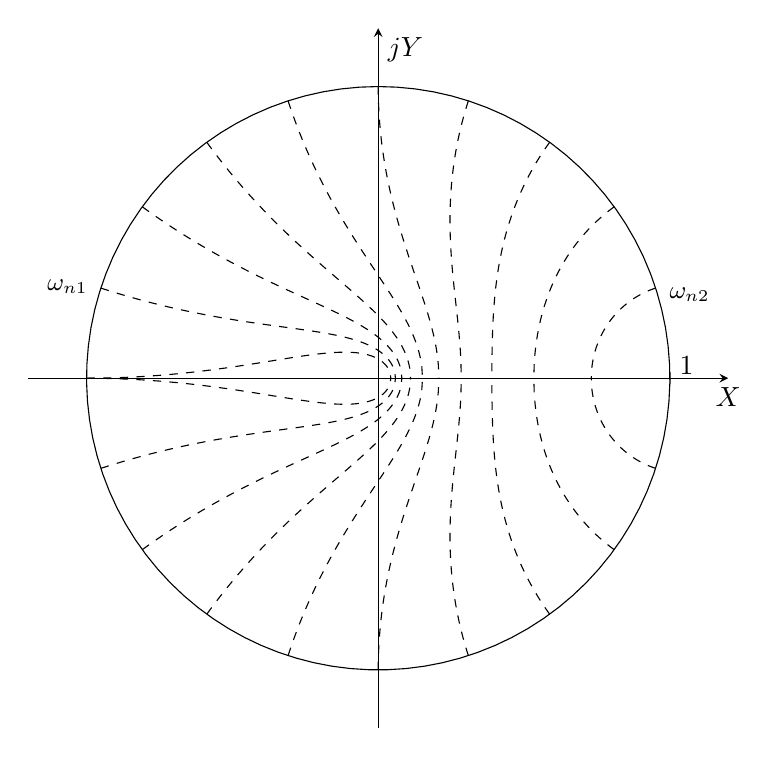
\begin{tikzpicture}

\begin{axis}[%
  axis lines=center,
  width=3.5in,
  height=3.5in,
  scale only axis,
  xmin=-1.2,
  xmax=1.2,
  ymin=-1.2,
  ymax=1.2,
  xtick={1},
  ytick=\empty,
  %xticklabels={},
  xticklabel style={anchor=south west},
  x label style={anchor=north},
  xlabel={$\pmb{X}$},
  ylabel={$\pmb{jY}$}
  ]
  \addplot [color=black, forget plot]
    table[row sep=crcr]{%
  0	1\\
  0.0634239196565645	0.997986676471884\\
  0.126592453573749	0.991954812830795\\
  0.18925124436041	0.981928697262707\\
  0.251147987181079	0.967948701396356\\
  0.312033445698487	0.950071117740945\\
  0.371662455660328	0.928367933016073\\
  0.429794912089172	0.902926538286621\\
  0.486196736100469	0.873849377069785\\
  0.540640817455598	0.841253532831181\\
  0.59290792905464	0.805270257531059\\
  0.642787609686539	0.766044443118978\\
  0.690079011482112	0.72373403810507\\
  0.734591708657533	0.678509411557132\\
  0.776146464291757	0.630552667084523\\
  0.814575952050336	0.580056909571198\\
  0.849725429949514	0.527225467610502\\
  0.881453363447582	0.472271074772683\\
  0.909631995354518	0.415415013001886\\
  0.934147860265107	0.356886221591872\\
  0.954902241444074	0.296920375328275\\
  0.971811568323542	0.235758935509427\\
  0.984807753012208	0.173648177666931\\
  0.993838464461254	0.110838199901011\\
  0.998867339183008	0.0475819158237424\\
  0.999874127673875	-0.015865963834808\\
  0.996854775951942	-0.0792499568567885\\
  0.989821441880933	-0.142314838273285\\
  0.978802446214779	-0.204806668065191\\
  0.963842158559942	-0.266473813690035\\
  0.945000818714669	-0.327067963317421\\
  0.922354294104581	-0.386345125693128\\
  0.895993774291336	-0.444066612605774\\
  0.866025403784439	-0.5\\
  0.832569854634771	-0.55392006386611\\
  0.795761840530832	-0.605609687137666\\
  0.755749574354258	-0.654860733945285\\
  0.712694171378863	-0.701474887706321\\
  0.666769000516292	-0.745264449675755\\
  0.618158986220605	-0.786053094742787\\
  0.567059863862771	-0.823676581429833\\
  0.513677391573407	-0.857983413234977\\
  0.458226521727411	-0.888835448654923\\
  0.400930535406614	-0.916108457432069\\
  0.342020143325669	-0.939692620785908\\
  0.28173255684143	-0.959492973614497\\
  0.220310532786541	-0.975429786885407\\
  0.15800139597335	-0.987438888676394\\
  0.0950560433041829	-0.995471922573085\\
  0.0317279334980681	-0.999496542383185\\
  -0.0317279334980679	-0.999496542383185\\
  -0.0950560433041826	-0.995471922573085\\
  -0.15800139597335	-0.987438888676394\\
  -0.220310532786541	-0.975429786885407\\
  -0.281732556841429	-0.959492973614497\\
  -0.342020143325669	-0.939692620785908\\
  -0.400930535406613	-0.91610845743207\\
  -0.45822652172741	-0.888835448654924\\
  -0.513677391573406	-0.857983413234977\\
  -0.567059863862771	-0.823676581429833\\
  -0.618158986220605	-0.786053094742788\\
  -0.666769000516292	-0.745264449675755\\
  -0.712694171378863	-0.701474887706322\\
  -0.755749574354258	-0.654860733945285\\
  -0.795761840530832	-0.605609687137667\\
  -0.832569854634771	-0.55392006386611\\
  -0.866025403784438	-0.5\\
  -0.895993774291336	-0.444066612605774\\
  -0.922354294104581	-0.386345125693129\\
  -0.945000818714668	-0.327067963317422\\
  -0.963842158559942	-0.266473813690035\\
  -0.978802446214779	-0.204806668065191\\
  -0.989821441880933	-0.142314838273285\\
  -0.996854775951942	-0.0792499568567888\\
  -0.999874127673875	-0.0158659638348076\\
  -0.998867339183008	0.0475819158237424\\
  -0.993838464461254	0.110838199901011\\
  -0.984807753012208	0.17364817766693\\
  -0.971811568323542	0.235758935509427\\
  -0.954902241444074	0.296920375328275\\
  -0.934147860265107	0.356886221591872\\
  -0.909631995354519	0.415415013001886\\
  -0.881453363447582	0.472271074772682\\
  -0.849725429949514	0.527225467610502\\
  -0.814575952050336	0.580056909571198\\
  -0.776146464291757	0.630552667084522\\
  -0.734591708657534	0.678509411557132\\
  -0.690079011482113	0.723734038105069\\
  -0.64278760968654	0.766044443118977\\
  -0.59290792905464	0.805270257531059\\
  -0.540640817455597	0.841253532831181\\
  -0.486196736100469	0.873849377069785\\
  -0.429794912089172	0.902926538286621\\
  -0.371662455660328	0.928367933016072\\
  -0.312033445698487	0.950071117740945\\
  -0.251147987181079	0.967948701396356\\
  -0.189251244360411	0.981928697262707\\
  -0.12659245357375	0.991954812830795\\
  -0.0634239196565654	0.997986676471884\\
  -2.44929359829471e-16	1\\
  };
  \addplot [color=black, dashed, forget plot]
    table[row sep=crcr]{%
  1	0\\
  1	0\\
  1	0\\
  1	0\\
  1	0\\
  1	0\\
  1	0\\
  1	0\\
  1	0\\
  1	0\\
  1	0\\
  1	0\\
  1	0\\
  1	0\\
  1	0\\
  1	0\\
  1	0\\
  1	0\\
  1	0\\
  1	0\\
  1	0\\
  1	0\\
  1	0\\
  1	0\\
  1	0\\
  1	0\\
  1	0\\
  1	0\\
  1	0\\
  1	0\\
  1	0\\
  1	0\\
  1	0\\
  1	0\\
  1	0\\
  1	0\\
  1	0\\
  1	0\\
  1	0\\
  1	0\\
  1	0\\
  1	0\\
  1	0\\
  1	0\\
  1	0\\
  1	0\\
  1	0\\
  1	0\\
  1	0\\
  1	0\\
  1	0\\
  1	0\\
  1	0\\
  1	0\\
  1	0\\
  1	0\\
  1	0\\
  1	0\\
  1	0\\
  1	0\\
  1	0\\
  1	0\\
  1	0\\
  1	0\\
  1	0\\
  1	0\\
  1	0\\
  1	0\\
  1	0\\
  1	0\\
  1	0\\
  1	0\\
  1	0\\
  1	0\\
  1	0\\
  1	0\\
  1	0\\
  1	0\\
  1	0\\
  1	0\\
  1	0\\
  1	0\\
  1	0\\
  1	0\\
  1	0\\
  1	0\\
  1	0\\
  1	0\\
  1	0\\
  1	0\\
  1	0\\
  1	0\\
  1	0\\
  1	0\\
  1	0\\
  1	0\\
  1	0\\
  1	0\\
  1	0\\
  1	0\\
  1	0\\
  };
  \addplot [color=black, dashed, forget plot]
    table[row sep=crcr]{%
  1	-0\\
  1	-0\\
  1	-0\\
  1	-0\\
  1	-0\\
  1	-0\\
  1	-0\\
  1	-0\\
  1	-0\\
  1	-0\\
  1	-0\\
  1	-0\\
  1	-0\\
  1	-0\\
  1	-0\\
  1	-0\\
  1	-0\\
  1	-0\\
  1	-0\\
  1	-0\\
  1	-0\\
  1	-0\\
  1	-0\\
  1	-0\\
  1	-0\\
  1	-0\\
  1	-0\\
  1	-0\\
  1	-0\\
  1	-0\\
  1	-0\\
  1	-0\\
  1	-0\\
  1	-0\\
  1	-0\\
  1	-0\\
  1	-0\\
  1	-0\\
  1	-0\\
  1	-0\\
  1	-0\\
  1	-0\\
  1	-0\\
  1	-0\\
  1	-0\\
  1	-0\\
  1	-0\\
  1	-0\\
  1	-0\\
  1	-0\\
  1	-0\\
  1	-0\\
  1	-0\\
  1	-0\\
  1	-0\\
  1	-0\\
  1	-0\\
  1	-0\\
  1	-0\\
  1	-0\\
  1	-0\\
  1	-0\\
  1	-0\\
  1	-0\\
  1	-0\\
  1	-0\\
  1	-0\\
  1	-0\\
  1	-0\\
  1	-0\\
  1	-0\\
  1	-0\\
  1	-0\\
  1	-0\\
  1	-0\\
  1	-0\\
  1	-0\\
  1	-0\\
  1	-0\\
  1	-0\\
  1	-0\\
  1	-0\\
  1	-0\\
  1	-0\\
  1	-0\\
  1	-0\\
  1	-0\\
  1	-0\\
  1	-0\\
  1	-0\\
  1	-0\\
  1	-0\\
  1	-0\\
  1	-0\\
  1	-0\\
  1	-0\\
  1	-0\\
  1	-0\\
  1	-0\\
  1	-0\\
  1	-0\\
  };
  \addplot [color=black, dashed, forget plot]
    table[row sep=crcr]{%
  0.951056516295154	0.309016994374947\\
  0.948078211301426	0.308032819485629\\
  0.94511888037394	0.307022081427976\\
  0.94217840366768	0.305985034984172\\
  0.939256662092049	0.30492192361348\\
  0.936353537306121	0.303832979577804\\
  0.933468911713929	0.302718424052102\\
  0.930602668459788	0.301578467219792\\
  0.927754691423642	0.30041330835324\\
  0.924924865216435	0.299223135879386\\
  0.922113075175525	0.298008127430492\\
  0.919319207360115	0.296768449879946\\
  0.916543148546715	0.295504259363022\\
  0.913784786224637	0.294215701282409\\
  0.911044008591513	0.292902910298318\\
  0.908320704548844	0.29156601030284\\
  0.905614763697579	0.29020511437826\\
  0.902926076333714	0.288820324738888\\
  0.900254533443929	0.287411732655945\\
  0.897600026701241	0.28597941836497\\
  0.894962448460698	0.284523450955115\\
  0.892341691755087	0.283043888239634\\
  0.889737650290675	0.281540776606779\\
  0.887150218442978	0.280014150850231\\
  0.884579291252554	0.278464033978077\\
  0.882024764420821	0.276890436999237\\
  0.879486534305908	0.275293358686166\\
  0.876964497918523	0.273672785312444\\
  0.874458552917854	0.272028690363831\\
  0.871968597607491	0.270361034221102\\
  0.869494530931379	0.268669763812905\\
  0.867036252469787	0.266954812236614\\
  0.864593662435318	0.265216098345006\\
  0.862166661668925	0.26345352629632\\
  0.859755151635967	0.261666985065034\\
  0.857359034422282	0.259856347910378\\
  0.85497821273029	0.258021471799335\\
  0.852612589875111	0.256162196780482\\
  0.850262069780723	0.25427834530468\\
  0.847926556976125	0.252369721488147\\
  0.845605956591542	0.250436110312975\\
  0.843300174354642	0.248477276759611\\
  0.84100911658678	0.246492964865175\\
  0.838732690199269	0.244482896700812\\
  0.836470802689669	0.24244677126046\\
  0.834223362138104	0.240384263252536\\
  0.831990277203598	0.238295021785015\\
  0.829771457120436	0.236178668933188\\
  0.82756681169455	0.234034798178102\\
  0.825376251299925	0.231862972702111\\
  0.823199686875027	0.22966272352627\\
  0.821037029919253	0.227433547472237\\
  0.818888192489409	0.225174904929094\\
  0.816753087196205	0.222886217402748\\
  0.814631627200769	0.22056686482251\\
  0.812523726211192	0.218216182575799\\
  0.810429298479085	0.215833458237678\\
  0.808348258796166	0.213417927956994\\
  0.806280522490864	0.210968772455044\\
  0.804226005424942	0.20848511258581\\
  0.802184623990148	0.205966004398664\\
  0.800156295104881	0.203410433634767\\
  0.798140936210878	0.200817309576802\\
  0.79613846526993	0.198185458157835\\
  0.794148800760608	0.195513614218404\\
  0.792171861675014	0.192800412780721\\
  0.790207567515554	0.190044379184321\\
  0.788255838291729	0.187243917897442\\
  0.78631659451695	0.184397299781511\\
  0.784389757205364	0.181502647540445\\
  0.78247524786871	0.178557919029679\\
  0.78057298851319	0.175560888028661\\
  0.778682901636361	0.172509121990832\\
  0.776804910224043	0.169399956171062\\
  0.774938937747252	0.166230463384427\\
  0.773084908159148	0.162997418461557\\
  0.771242745892004	0.159697256219759\\
  0.769412375854194	0.156326021445345\\
  0.7675937234272	0.15287930895176\\
  0.765786714462635	0.14935219119843\\
  0.763991275279289	0.145739130165498\\
  0.762207332660193	0.142033869089184\\
  0.760434813849697	0.138229298134639\\
  0.75867364655057	0.134317285907685\\
  0.756923758921121	0.130288465553936\\
  0.755185079572328	0.126131959533784\\
  0.753457537565001	0.121835020122195\\
  0.751741062406945	0.117382551784649\\
  0.750035584050153	0.11275646423786\\
  0.748341032888014	0.107934776522348\\
  0.746657339752536	0.102890343917207\\
  0.744984435911586	0.0975889934047091\\
  0.743322253066156	0.0919866926847057\\
  0.741670723347631	0.0860250595183118\\
  0.740029779315089	0.0796238406412504\\
  0.738399353952608	0.0726674092994395\\
  0.736779380666597	0.0649781812312819\\
  0.735169793283135	0.0562570328679831\\
  0.733570526045337	0.0459203986166819\\
  0.73198151361073	0.0324609316188515\\
  0.730402691048646	0\\
  };
  \addplot [color=black, dashed, forget plot]
    table[row sep=crcr]{%
  0.951056516295154	-0.309016994374947\\
  0.948078211301426	-0.308032819485629\\
  0.94511888037394	-0.307022081427976\\
  0.94217840366768	-0.305985034984172\\
  0.939256662092049	-0.30492192361348\\
  0.936353537306121	-0.303832979577804\\
  0.933468911713929	-0.302718424052102\\
  0.930602668459788	-0.301578467219792\\
  0.927754691423642	-0.30041330835324\\
  0.924924865216435	-0.299223135879386\\
  0.922113075175525	-0.298008127430492\\
  0.919319207360115	-0.296768449879946\\
  0.916543148546715	-0.295504259363022\\
  0.913784786224637	-0.294215701282409\\
  0.911044008591513	-0.292902910298318\\
  0.908320704548844	-0.29156601030284\\
  0.905614763697579	-0.29020511437826\\
  0.902926076333714	-0.288820324738888\\
  0.900254533443929	-0.287411732655945\\
  0.897600026701241	-0.28597941836497\\
  0.894962448460698	-0.284523450955115\\
  0.892341691755087	-0.283043888239634\\
  0.889737650290675	-0.281540776606779\\
  0.887150218442978	-0.280014150850231\\
  0.884579291252554	-0.278464033978077\\
  0.882024764420821	-0.276890436999237\\
  0.879486534305908	-0.275293358686166\\
  0.876964497918523	-0.273672785312444\\
  0.874458552917854	-0.272028690363831\\
  0.871968597607491	-0.270361034221102\\
  0.869494530931379	-0.268669763812905\\
  0.867036252469787	-0.266954812236614\\
  0.864593662435318	-0.265216098345006\\
  0.862166661668925	-0.26345352629632\\
  0.859755151635967	-0.261666985065034\\
  0.857359034422282	-0.259856347910378\\
  0.85497821273029	-0.258021471799335\\
  0.852612589875111	-0.256162196780482\\
  0.850262069780723	-0.25427834530468\\
  0.847926556976125	-0.252369721488147\\
  0.845605956591542	-0.250436110312975\\
  0.843300174354642	-0.248477276759611\\
  0.84100911658678	-0.246492964865175\\
  0.838732690199269	-0.244482896700812\\
  0.836470802689669	-0.24244677126046\\
  0.834223362138104	-0.240384263252536\\
  0.831990277203598	-0.238295021785015\\
  0.829771457120436	-0.236178668933188\\
  0.82756681169455	-0.234034798178102\\
  0.825376251299925	-0.231862972702111\\
  0.823199686875027	-0.22966272352627\\
  0.821037029919253	-0.227433547472237\\
  0.818888192489409	-0.225174904929094\\
  0.816753087196205	-0.222886217402748\\
  0.814631627200769	-0.22056686482251\\
  0.812523726211192	-0.218216182575799\\
  0.810429298479085	-0.215833458237678\\
  0.808348258796166	-0.213417927956994\\
  0.806280522490864	-0.210968772455044\\
  0.804226005424942	-0.20848511258581\\
  0.802184623990148	-0.205966004398664\\
  0.800156295104881	-0.203410433634767\\
  0.798140936210878	-0.200817309576802\\
  0.79613846526993	-0.198185458157835\\
  0.794148800760608	-0.195513614218404\\
  0.792171861675014	-0.192800412780721\\
  0.790207567515554	-0.190044379184321\\
  0.788255838291729	-0.187243917897442\\
  0.78631659451695	-0.184397299781511\\
  0.784389757205364	-0.181502647540445\\
  0.78247524786871	-0.178557919029679\\
  0.78057298851319	-0.175560888028661\\
  0.778682901636361	-0.172509121990832\\
  0.776804910224043	-0.169399956171062\\
  0.774938937747252	-0.166230463384427\\
  0.773084908159148	-0.162997418461557\\
  0.771242745892004	-0.159697256219759\\
  0.769412375854194	-0.156326021445345\\
  0.7675937234272	-0.15287930895176\\
  0.765786714462635	-0.14935219119843\\
  0.763991275279289	-0.145739130165498\\
  0.762207332660193	-0.142033869089184\\
  0.760434813849697	-0.138229298134639\\
  0.75867364655057	-0.134317285907685\\
  0.756923758921121	-0.130288465553936\\
  0.755185079572328	-0.126131959533784\\
  0.753457537565001	-0.121835020122195\\
  0.751741062406945	-0.117382551784649\\
  0.750035584050153	-0.11275646423786\\
  0.748341032888014	-0.107934776522348\\
  0.746657339752536	-0.102890343917207\\
  0.744984435911586	-0.0975889934047091\\
  0.743322253066156	-0.0919866926847057\\
  0.741670723347631	-0.0860250595183118\\
  0.740029779315089	-0.0796238406412504\\
  0.738399353952608	-0.0726674092994395\\
  0.736779380666597	-0.0649781812312819\\
  0.735169793283135	-0.0562570328679831\\
  0.733570526045337	-0.0459203986166819\\
  0.73198151361073	-0.0324609316188515\\
  0.730402691048646	-0\\
  };
  \addplot [color=black, dashed, forget plot]
    table[row sep=crcr]{%
  0.809016994374947	0.587785252292473\\
  0.803968076864246	0.584078409040141\\
  0.798987139554922	0.580344731698571\\
  0.794073302703513	0.576584983615173\\
  0.789225697784154	0.572799896343767\\
  0.784443467346559	0.568990170355869\\
  0.779725764875798	0.565156475711343\\
  0.775071754653839	0.561299452689503\\
  0.770480611622838	0.55741971238163\\
  0.765951521250147	0.55351783724576\\
  0.761483679395036	0.549594381624462\\
  0.757076292177084	0.545649872226245\\
  0.752728575846238	0.541684808571098\\
  0.748439756654506	0.537699663400556\\
  0.744209070729268	0.533694883052599\\
  0.740035763948193	0.529670887801542\\
  0.735919091815723	0.525628072162995\\
  0.73185831934112	0.521566805163826\\
  0.727852720918053	0.517487430576977\\
  0.723901580205702	0.513390267120805\\
  0.72000419001136	0.509275608622555\\
  0.716159852174521	0.505143724145385\\
  0.712367877452424	0.500994858078254\\
  0.708627585407048	0.496829230187816\\
  0.704938304293527	0.492647035631308\\
  0.701299370949976	0.488448444929261\\
  0.697710130688707	0.484233603896658\\
  0.694169937188816	0.480002633530983\\
  0.690678152390127	0.475755629855389\\
  0.687234146388471	0.471492663714971\\
  0.683837297332295	0.467213780523892\\
  0.680486991320567	0.462918999960819\\
  0.677182622301969	0.458608315609828\\
  0.673923591975373	0.45428169454361\\
  0.67070930969156	0.449939076845429\\
  0.667539192356189	0.445580375065885\\
  0.664412664333986	0.441205473610068\\
  0.661329157354143	0.436814228050209\\
  0.658288110416912	0.43240646435835\\
  0.655288969701381	0.427981978052936\\
  0.652331188474404	0.423540533252536\\
  0.649414227000697	0.419081861629092\\
  0.646537552454051	0.414605661252235\\
  0.643700638829683	0.410111595315165\\
  0.640902966857678	0.405599290731511\\
  0.638144023917538	0.401068336591244\\
  0.635423303953798	0.396518282462304\\
  0.632740307392718	0.391948636522913\\
  0.630094541060018	0.387358863507658\\
  0.627485518099657	0.382748382448251\\
  0.624912757893638	0.378116564187382\\
  0.622375785982821	0.37346272864121\\
  0.619874133988746	0.368786141782721\\
  0.617407339536427	0.364086012314358\\
  0.614974946178141	0.359361487993868\\
  0.612576503318165	0.35461165157214\\
  0.610211566138466	0.349835516295752\\
  0.607879695525337	0.345032020919843\\
  0.605580457996952	0.340200024168619\\
  0.603313425631842	0.335338298570911\\
  0.601078175998265	0.330445523586591\\
  0.598874292084485	0.325520277925745\\
  0.596701362229912	0.320561030945957\\
  0.594558980057129	0.315566132993194\\
  0.592446744404769	0.310533804527835\\
  0.590364259261241	0.305462123848429\\
  0.588311133699294	0.300349013190491\\
  0.586286981811413	0.295192222934552\\
  0.584291422646021	0.289989313604637\\
  0.582324080144498	0.284737635272761\\
  0.580384583078989	0.279434303903338\\
  0.578472564991001	0.274076174069122\\
  0.576587664130775	0.268659807341124\\
  0.574729523397425	0.263181435490837\\
  0.572897790279837	0.257636917432723\\
  0.571092116798306	0.252021688563062\\
  0.569312159446919	0.246330700796692\\
  0.567557579136666	0.240558351136193\\
  0.565828041139265	0.234698395986517\\
  0.564123215031705	0.228743847591282\\
  0.562442774641479	0.222686847826466\\
  0.560786397992523	0.216518513011748\\
  0.559153767251828	0.210228741191177\\
  0.557544568676733	0.203805970188717\\
  0.555958492562879	0.1972368701823\\
  0.554395233192832	0.190505947794269\\
  0.55285448878534	0.183595028500902\\
  0.551335961445247	0.17648256837326\\
  0.549839357114031	0.169142721020148\\
  0.548364385520971	0.161544044294541\\
  0.546910760134932	0.15364766095089\\
  0.54547819811676	0.145404562405573\\
  0.544066420272276	0.136751511316999\\
  0.542675151005869	0.127604536237939\\
  0.541304118274676	0.117848026435929\\
  0.539953053543337	0.107315136160232\\
  0.538621691739329	0.0957491682488516\\
  0.537309771208858	0.0827169424485554\\
  0.536017033673318	0.0673717019389019\\
  0.534743224186292	0.0475216037191627\\
  0.533488091091103	0\\
  };
  \addplot [color=black, dashed, forget plot]
    table[row sep=crcr]{%
  0.809016994374947	-0.587785252292473\\
  0.803968076864246	-0.584078409040141\\
  0.798987139554922	-0.580344731698571\\
  0.794073302703513	-0.576584983615173\\
  0.789225697784154	-0.572799896343767\\
  0.784443467346559	-0.568990170355869\\
  0.779725764875798	-0.565156475711343\\
  0.775071754653839	-0.561299452689503\\
  0.770480611622838	-0.55741971238163\\
  0.765951521250147	-0.55351783724576\\
  0.761483679395036	-0.549594381624462\\
  0.757076292177084	-0.545649872226245\\
  0.752728575846238	-0.541684808571098\\
  0.748439756654506	-0.537699663400556\\
  0.744209070729268	-0.533694883052599\\
  0.740035763948193	-0.529670887801542\\
  0.735919091815723	-0.525628072162995\\
  0.73185831934112	-0.521566805163826\\
  0.727852720918053	-0.517487430576977\\
  0.723901580205702	-0.513390267120805\\
  0.72000419001136	-0.509275608622555\\
  0.716159852174521	-0.505143724145385\\
  0.712367877452424	-0.500994858078254\\
  0.708627585407048	-0.496829230187816\\
  0.704938304293527	-0.492647035631308\\
  0.701299370949976	-0.488448444929261\\
  0.697710130688707	-0.484233603896658\\
  0.694169937188816	-0.480002633530983\\
  0.690678152390127	-0.475755629855389\\
  0.687234146388471	-0.471492663714971\\
  0.683837297332295	-0.467213780523892\\
  0.680486991320567	-0.462918999960819\\
  0.677182622301969	-0.458608315609828\\
  0.673923591975373	-0.45428169454361\\
  0.67070930969156	-0.449939076845429\\
  0.667539192356189	-0.445580375065885\\
  0.664412664333986	-0.441205473610068\\
  0.661329157354143	-0.436814228050209\\
  0.658288110416912	-0.43240646435835\\
  0.655288969701381	-0.427981978052936\\
  0.652331188474404	-0.423540533252536\\
  0.649414227000697	-0.419081861629092\\
  0.646537552454051	-0.414605661252235\\
  0.643700638829683	-0.410111595315165\\
  0.640902966857678	-0.405599290731511\\
  0.638144023917538	-0.401068336591244\\
  0.635423303953798	-0.396518282462304\\
  0.632740307392718	-0.391948636522913\\
  0.630094541060018	-0.387358863507658\\
  0.627485518099657	-0.382748382448251\\
  0.624912757893638	-0.378116564187382\\
  0.622375785982821	-0.37346272864121\\
  0.619874133988746	-0.368786141782721\\
  0.617407339536427	-0.364086012314358\\
  0.614974946178141	-0.359361487993868\\
  0.612576503318165	-0.35461165157214\\
  0.610211566138466	-0.349835516295752\\
  0.607879695525337	-0.345032020919843\\
  0.605580457996952	-0.340200024168619\\
  0.603313425631842	-0.335338298570911\\
  0.601078175998265	-0.330445523586591\\
  0.598874292084485	-0.325520277925745\\
  0.596701362229912	-0.320561030945957\\
  0.594558980057129	-0.315566132993194\\
  0.592446744404769	-0.310533804527835\\
  0.590364259261241	-0.305462123848429\\
  0.588311133699294	-0.300349013190491\\
  0.586286981811413	-0.295192222934552\\
  0.584291422646021	-0.289989313604637\\
  0.582324080144498	-0.284737635272761\\
  0.580384583078989	-0.279434303903338\\
  0.578472564991001	-0.274076174069122\\
  0.576587664130775	-0.268659807341124\\
  0.574729523397425	-0.263181435490837\\
  0.572897790279837	-0.257636917432723\\
  0.571092116798306	-0.252021688563062\\
  0.569312159446919	-0.246330700796692\\
  0.567557579136666	-0.240558351136193\\
  0.565828041139265	-0.234698395986517\\
  0.564123215031705	-0.228743847591282\\
  0.562442774641479	-0.222686847826466\\
  0.560786397992523	-0.216518513011748\\
  0.559153767251828	-0.210228741191177\\
  0.557544568676733	-0.203805970188717\\
  0.555958492562879	-0.1972368701823\\
  0.554395233192832	-0.190505947794269\\
  0.55285448878534	-0.183595028500902\\
  0.551335961445247	-0.17648256837326\\
  0.549839357114031	-0.169142721020148\\
  0.548364385520971	-0.161544044294541\\
  0.546910760134932	-0.15364766095089\\
  0.54547819811676	-0.145404562405573\\
  0.544066420272276	-0.136751511316999\\
  0.542675151005869	-0.127604536237939\\
  0.541304118274676	-0.117848026435929\\
  0.539953053543337	-0.107315136160232\\
  0.538621691739329	-0.0957491682488516\\
  0.537309771208858	-0.0827169424485554\\
  0.536017033673318	-0.0673717019389019\\
  0.534743224186292	-0.0475216037191627\\
  0.533488091091103	-0\\
  };
  \addplot [color=black, dashed, forget plot]
    table[row sep=crcr]{%
  0.587785252292473	0.809016994374947\\
  0.582309297119587	0.801400566795492\\
  0.576959183297469	0.793801457674205\\
  0.571732340353481	0.786220466749031\\
  0.56662624829927	0.778658336620054\\
  0.561638436656923	0.771115754699379\\
  0.556766483503744	0.763593355066369\\
  0.552008014535265	0.75609172023173\\
  0.547360702146168	0.748611382813718\\
  0.542822264528764	0.741152827129482\\
  0.538390464788706	0.733716490704319\\
  0.534063110077599	0.726302765701431\\
  0.529838050742194	0.718912000274504\\
  0.525713179489847	0.711544499845278\\
  0.52168643056993	0.704200528308028\\
  0.517755778970906	0.696880309162698\\
  0.513919239632746	0.689584026578232\\
  0.510174866674423	0.682311826387443\\
  0.506520752636174	0.675063817014576\\
  0.502955027736264	0.667840070336502\\
  0.499475859141973	0.660640622478329\\
  0.496081450254526	0.653465474543956\\
  0.492770040007721	0.646314593281934\\
  0.489539902179967	0.639187911686782\\
  0.48638934471951	0.632085329535654\\
  0.483316709082561	0.625006713860077\\
  0.480320369584116	0.61795189935219\\
  0.477398732761191	0.610920688704696\\
  0.474550236748266	0.603912852883462\\
  0.471773350664695	0.596928131331407\\
  0.469066574013837	0.589966232102021\\
  0.466428436093723	0.583026831920531\\
  0.463857495418998	0.576109576170361\\
  0.461352339153956	0.569214078802161\\
  0.458911582556433	0.56233992216223\\
  0.456533868432375	0.555486656736729\\
  0.454217866600849	0.548653800807529\\
  0.451962273369329	0.541840840015008\\
  0.449765811019036	0.535047226822452\\
  0.447627227300158	0.528272379876049\\
  0.445545294936748	0.521515683253672\\
  0.443518811141127	0.514776485594762\\
  0.441546597137611	0.508054099102692\\
  0.439627497695365	0.501347798409846\\
  0.437760380670245	0.494656819294441\\
  0.435944136555421	0.487980357236711\\
  0.434177678040635	0.481317565800483\\
  0.432459939579929	0.474667554824374\\
  0.430789876967667	0.468029388404762\\
  0.42916646692271	0.461402082650359\\
  0.427588706680582	0.454784603185479\\
  0.426055613593464	0.448175862376014\\
  0.42456622473789	0.441574716248516\\
  0.423119596529975	0.434979961068675\\
  0.421714804348045	0.428390329540639\\
  0.420350942162526	0.421804486583022\\
  0.419027122172945	0.415221024630929\\
  0.417742474451922	0.408638458405624\\
  0.41649614659601	0.402055219084459\\
  0.415287303383244	0.395469647793065\\
  0.414115126437298	0.388879988329137\\
  0.412978813898094	0.382284379012195\\
  0.411877580098755	0.375680843535754\\
  0.410810655248786	0.369067280676845\\
  0.409777285123346	0.362441452691912\\
  0.408776730758515	0.355800972196766\\
  0.407808268152427	0.349143287290061\\
  0.406871187972163	0.342465664633109\\
  0.405964795266295	0.33576517014133\\
  0.405088409182968	0.329038646871611\\
  0.404241362693423	0.322282689601277\\
  0.403423002320843	0.315493615483433\\
  0.40263268787444	0.308667430023397\\
  0.401869792188659	0.301799787442834\\
  0.401133700867428	0.294885944269923\\
  0.40042381203333	0.287920704698758\\
  0.399739536081626	0.280898355876161\\
  0.399080295439023	0.273812590766852\\
  0.398445524327102	0.266656415572581\\
  0.39783466853031	0.259422037771358\\
  0.39724718516844	0.252100729602985\\
  0.396682542473503	0.244682660113701\\
  0.396140219570916	0.237156686470128\\
  0.395619706264911	0.229510091829081\\
  0.395120502828102	0.22172825208392\\
  0.394642119795116	0.213794206462818\\
  0.394184077760218	0.205688095849274\\
  0.393745907178842	0.197386415490307\\
  0.39332714817298	0.188861001355175\\
  0.392927350340317	0.180077624368305\\
  0.392546072567074	0.170993989987095\\
  0.392182882844471	0.161556804181116\\
  0.39183735808874	0.151697312104007\\
  0.391509083964633	0.14132421085842\\
  0.391197654712337	0.130311761848054\\
  0.390902672977758	0.118478416754367\\
  0.390623749646079	0.105544670782668\\
  0.390360503678557	0.0910384509401026\\
  0.390112561952479	0.0740360106835001\\
  0.389879559104218	0.0521431986535175\\
  0.389661137375347	0\\
  };
  \addplot [color=black, dashed, forget plot]
    table[row sep=crcr]{%
  0.587785252292473	-0.809016994374947\\
  0.582309297119587	-0.801400566795492\\
  0.576959183297469	-0.793801457674205\\
  0.571732340353481	-0.786220466749031\\
  0.56662624829927	-0.778658336620054\\
  0.561638436656923	-0.771115754699379\\
  0.556766483503744	-0.763593355066369\\
  0.552008014535265	-0.75609172023173\\
  0.547360702146168	-0.748611382813718\\
  0.542822264528764	-0.741152827129482\\
  0.538390464788706	-0.733716490704319\\
  0.534063110077599	-0.726302765701431\\
  0.529838050742194	-0.718912000274504\\
  0.525713179489847	-0.711544499845278\\
  0.52168643056993	-0.704200528308028\\
  0.517755778970906	-0.696880309162698\\
  0.513919239632746	-0.689584026578232\\
  0.510174866674423	-0.682311826387443\\
  0.506520752636174	-0.675063817014576\\
  0.502955027736264	-0.667840070336502\\
  0.499475859141973	-0.660640622478329\\
  0.496081450254526	-0.653465474543956\\
  0.492770040007721	-0.646314593281934\\
  0.489539902179967	-0.639187911686782\\
  0.48638934471951	-0.632085329535654\\
  0.483316709082561	-0.625006713860077\\
  0.480320369584116	-0.61795189935219\\
  0.477398732761191	-0.610920688704696\\
  0.474550236748266	-0.603912852883462\\
  0.471773350664695	-0.596928131331407\\
  0.469066574013837	-0.589966232102021\\
  0.466428436093723	-0.583026831920531\\
  0.463857495418998	-0.576109576170361\\
  0.461352339153956	-0.569214078802161\\
  0.458911582556433	-0.56233992216223\\
  0.456533868432375	-0.555486656736729\\
  0.454217866600849	-0.548653800807529\\
  0.451962273369329	-0.541840840015008\\
  0.449765811019036	-0.535047226822452\\
  0.447627227300158	-0.528272379876049\\
  0.445545294936748	-0.521515683253672\\
  0.443518811141127	-0.514776485594762\\
  0.441546597137611	-0.508054099102692\\
  0.439627497695365	-0.501347798409846\\
  0.437760380670245	-0.494656819294441\\
  0.435944136555421	-0.487980357236711\\
  0.434177678040635	-0.481317565800483\\
  0.432459939579929	-0.474667554824374\\
  0.430789876967667	-0.468029388404762\\
  0.42916646692271	-0.461402082650359\\
  0.427588706680582	-0.454784603185479\\
  0.426055613593464	-0.448175862376014\\
  0.42456622473789	-0.441574716248516\\
  0.423119596529975	-0.434979961068675\\
  0.421714804348045	-0.428390329540639\\
  0.420350942162526	-0.421804486583022\\
  0.419027122172945	-0.415221024630929\\
  0.417742474451922	-0.408638458405624\\
  0.41649614659601	-0.402055219084459\\
  0.415287303383244	-0.395469647793065\\
  0.414115126437298	-0.388879988329137\\
  0.412978813898094	-0.382284379012195\\
  0.411877580098755	-0.375680843535754\\
  0.410810655248786	-0.369067280676845\\
  0.409777285123346	-0.362441452691912\\
  0.408776730758515	-0.355800972196766\\
  0.407808268152427	-0.349143287290061\\
  0.406871187972163	-0.342465664633109\\
  0.405964795266295	-0.33576517014133\\
  0.405088409182968	-0.329038646871611\\
  0.404241362693423	-0.322282689601277\\
  0.403423002320843	-0.315493615483433\\
  0.40263268787444	-0.308667430023397\\
  0.401869792188659	-0.301799787442834\\
  0.401133700867428	-0.294885944269923\\
  0.40042381203333	-0.287920704698758\\
  0.399739536081626	-0.280898355876161\\
  0.399080295439023	-0.273812590766852\\
  0.398445524327102	-0.266656415572581\\
  0.39783466853031	-0.259422037771358\\
  0.39724718516844	-0.252100729602985\\
  0.396682542473503	-0.244682660113701\\
  0.396140219570916	-0.237156686470128\\
  0.395619706264911	-0.229510091829081\\
  0.395120502828102	-0.22172825208392\\
  0.394642119795116	-0.213794206462818\\
  0.394184077760218	-0.205688095849274\\
  0.393745907178842	-0.197386415490307\\
  0.39332714817298	-0.188861001355175\\
  0.392927350340317	-0.180077624368305\\
  0.392546072567074	-0.170993989987095\\
  0.392182882844471	-0.161556804181116\\
  0.39183735808874	-0.151697312104007\\
  0.391509083964633	-0.14132421085842\\
  0.391197654712337	-0.130311761848054\\
  0.390902672977758	-0.118478416754367\\
  0.390623749646079	-0.105544670782668\\
  0.390360503678557	-0.0910384509401026\\
  0.390112561952479	-0.0740360106835001\\
  0.389879559104218	-0.0521431986535175\\
  0.389661137375347	-0\\
  };
  \addplot [color=black, dashed, forget plot]
    table[row sep=crcr]{%
  0.309016994374947	0.951056516295154\\
  0.305217080709932	0.939160790507861\\
  0.30158044156387	0.92737595427122\\
  0.298102166735956	0.915701484457103\\
  0.294777480791454	0.904136795765201\\
  0.29160173950109	0.892681244240134\\
  0.288570426372682	0.881334130597075\\
  0.285679149272646	0.870094703364585\\
  0.282923637135083	0.858962161852849\\
  0.280299736756191	0.847935658954962\\
  0.277803409671828	0.837014303788469\\
  0.275430729116085	0.826197164183891\\
  0.273177877058799	0.81548326902653\\
  0.271041141319984	0.804871610457444\\
  0.269016912759193	0.794361145939081\\
  0.267101682537912	0.783950800190664\\
  0.265292039453092	0.77363946699808\\
  0.263584667340008	0.763426010902631\\
  0.261976342542652	0.75330926877269\\
  0.260463931449941	0.743288051261957\\
  0.259044388096041	0.733361144157651\\
  0.257714751823163	0.723527309621692\\
  0.256472145005221	0.713785287327568\\
  0.255313770830805	0.704133795495268\\
  0.254236911143918	0.694571531826333\\
  0.253238924341019	0.68509717434077\\
  0.252317243322908	0.675709382117202\\
  0.251469373500046	0.666406795937338\\
  0.250692890849941	0.657188038835442\\
  0.249985440025252	0.648051716553169\\
  0.249344732511311	0.638996417899726\\
  0.248768544831792	0.630020715016927\\
  0.248254716801288	0.621123163548305\\
  0.247801149823575	0.612302302710977\\
  0.247405805234411	0.603556655268511\\
  0.247066702687698	0.594884727402498\\
  0.246781918583901	0.586285008480007\\
  0.246549584539641	0.57775597071349\\
  0.24636788589738	0.569296068709032\\
  0.246235060274193	0.560903738898134\\
  0.246149396148586	0.552577398847419\\
  0.246109231484407	0.54431544643974\\
  0.246112952390872	0.536116258919226\\
  0.246158991817792	0.527978191791664\\
  0.246245828285069	0.51989957757039\\
  0.2463719846456	0.5118787243565\\
  0.246536026880706	0.503913914240565\\
  0.246736562927261	0.49600340151133\\
  0.246972241535691	0.488145410654776\\
  0.247241751158043	0.480338134124693\\
  0.247543818865362	0.472579729863208\\
  0.247877209293596	0.464868318546725\\
  0.248240723617312	0.45720198052923\\
  0.248633198550478	0.449578752450869\\
  0.249053505373641	0.441996623475051\\
  0.249500548986788	0.434453531111882\\
  0.249973266987244	0.426947356579379\\
  0.250470628771945	0.419475919646492\\
  0.25099163466347	0.412036972893213\\
  0.251535315059195	0.404628195312739\\
  0.252100729602985	0.39724718516844\\
  0.252686966378838	0.389891452003851\\
  0.253293141125898	0.382558407686555\\
  0.253918396474296	0.375245356346011\\
  0.254561901201278	0.367949483040285\\
  0.25522284950708	0.360667840956287\\
  0.255900460310047	0.353397336911125\\
  0.256593976560494	0.346134714877\\
  0.257302664572823	0.338876537196393\\
  0.258025813375412	0.33161916308546\\
  0.258762734077829	0.324358723937813\\
  0.2595127592549	0.317091094833371\\
  0.260275242347213	0.309811861521285\\
  0.261049557077614	0.302516281973398\\
  0.261835096883284	0.295199241383432\\
  0.262631274362992	0.287855199201125\\
  0.263437520739125	0.280478126417275\\
  0.264253285334109	0.273061430823931\\
  0.265078035060854	0.265597867319157\\
  0.265911253926843	0.258079429443833\\
  0.266752442551518	0.250497217135365\\
  0.26760111769661	0.242841274021111\\
  0.268456811809085	0.235100385243312\\
  0.26931907257636	0.227261823485223\\
  0.27018746249348	0.219311026048744\\
  0.271061558441942	0.21123117870405\\
  0.271940951279852	0.203002671250792\\
  0.272825245443132	0.194602373024796\\
  0.273714058557471	0.186002649972472\\
  0.274607021060755	0.177170001168297\\
  0.27550377583569	0.168063118087211\\
  0.276403977852351	0.158630037397896\\
  0.277307293820405	0.148803810458127\\
  0.278213401850743	0.138495621943914\\
  0.279121991126281	0.127583244080622\\
  0.280032761581685	0.115890270922272\\
  0.28094542359179	0.10314515796966\\
  0.281859697668478	0.0888892428442591\\
  0.282775314165799	0.0722247596536262\\
  0.28369201299311	0.0508237111825767\\
  0.284609543336029	0\\
  };
  \addplot [color=black, dashed, forget plot]
    table[row sep=crcr]{%
  0.309016994374947	-0.951056516295154\\
  0.305217080709932	-0.939160790507861\\
  0.30158044156387	-0.92737595427122\\
  0.298102166735956	-0.915701484457103\\
  0.294777480791454	-0.904136795765201\\
  0.29160173950109	-0.892681244240134\\
  0.288570426372682	-0.881334130597075\\
  0.285679149272646	-0.870094703364585\\
  0.282923637135083	-0.858962161852849\\
  0.280299736756191	-0.847935658954962\\
  0.277803409671828	-0.837014303788469\\
  0.275430729116085	-0.826197164183891\\
  0.273177877058799	-0.81548326902653\\
  0.271041141319984	-0.804871610457444\\
  0.269016912759193	-0.794361145939081\\
  0.267101682537912	-0.783950800190664\\
  0.265292039453092	-0.77363946699808\\
  0.263584667340008	-0.763426010902631\\
  0.261976342542652	-0.75330926877269\\
  0.260463931449941	-0.743288051261957\\
  0.259044388096041	-0.733361144157651\\
  0.257714751823163	-0.723527309621692\\
  0.256472145005221	-0.713785287327568\\
  0.255313770830805	-0.704133795495268\\
  0.254236911143918	-0.694571531826333\\
  0.253238924341019	-0.68509717434077\\
  0.252317243322908	-0.675709382117202\\
  0.251469373500046	-0.666406795937338\\
  0.250692890849941	-0.657188038835442\\
  0.249985440025252	-0.648051716553169\\
  0.249344732511311	-0.638996417899726\\
  0.248768544831792	-0.630020715016927\\
  0.248254716801288	-0.621123163548305\\
  0.247801149823575	-0.612302302710977\\
  0.247405805234411	-0.603556655268511\\
  0.247066702687698	-0.594884727402498\\
  0.246781918583901	-0.586285008480007\\
  0.246549584539641	-0.57775597071349\\
  0.24636788589738	-0.569296068709032\\
  0.246235060274193	-0.560903738898134\\
  0.246149396148586	-0.552577398847419\\
  0.246109231484407	-0.54431544643974\\
  0.246112952390872	-0.536116258919226\\
  0.246158991817792	-0.527978191791664\\
  0.246245828285069	-0.51989957757039\\
  0.2463719846456	-0.5118787243565\\
  0.246536026880706	-0.503913914240565\\
  0.246736562927261	-0.49600340151133\\
  0.246972241535691	-0.488145410654776\\
  0.247241751158043	-0.480338134124693\\
  0.247543818865362	-0.472579729863208\\
  0.247877209293596	-0.464868318546725\\
  0.248240723617312	-0.45720198052923\\
  0.248633198550478	-0.449578752450869\\
  0.249053505373641	-0.441996623475051\\
  0.249500548986788	-0.434453531111882\\
  0.249973266987244	-0.426947356579379\\
  0.250470628771945	-0.419475919646492\\
  0.25099163466347	-0.412036972893213\\
  0.251535315059195	-0.404628195312739\\
  0.252100729602985	-0.39724718516844\\
  0.252686966378838	-0.389891452003851\\
  0.253293141125898	-0.382558407686555\\
  0.253918396474296	-0.375245356346011\\
  0.254561901201278	-0.367949483040285\\
  0.25522284950708	-0.360667840956287\\
  0.255900460310047	-0.353397336911125\\
  0.256593976560494	-0.346134714877\\
  0.257302664572823	-0.338876537196393\\
  0.258025813375412	-0.33161916308546\\
  0.258762734077829	-0.324358723937813\\
  0.2595127592549	-0.317091094833371\\
  0.260275242347213	-0.309811861521285\\
  0.261049557077614	-0.302516281973398\\
  0.261835096883284	-0.295199241383432\\
  0.262631274362992	-0.287855199201125\\
  0.263437520739125	-0.280478126417275\\
  0.264253285334109	-0.273061430823931\\
  0.265078035060854	-0.265597867319157\\
  0.265911253926843	-0.258079429443833\\
  0.266752442551518	-0.250497217135365\\
  0.26760111769661	-0.242841274021111\\
  0.268456811809085	-0.235100385243312\\
  0.26931907257636	-0.227261823485223\\
  0.27018746249348	-0.219311026048744\\
  0.271061558441942	-0.21123117870405\\
  0.271940951279852	-0.203002671250792\\
  0.272825245443132	-0.194602373024796\\
  0.273714058557471	-0.186002649972472\\
  0.274607021060755	-0.177170001168297\\
  0.27550377583569	-0.168063118087211\\
  0.276403977852351	-0.158630037397896\\
  0.277307293820405	-0.148803810458127\\
  0.278213401850743	-0.138495621943914\\
  0.279121991126281	-0.127583244080622\\
  0.280032761581685	-0.115890270922272\\
  0.28094542359179	-0.10314515796966\\
  0.281859697668478	-0.0888892428442591\\
  0.282775314165799	-0.0722247596536262\\
  0.28369201299311	-0.0508237111825767\\
  0.284609543336029	-0\\
  };
  \addplot [color=black, dashed, forget plot]
    table[row sep=crcr]{%
  6.12323399573677e-17	1\\
  7.7317687626911e-05	0.984414760315379\\
  0.000304473526916821	0.969072378473437\\
  0.000674472828493945	0.953968964779478\\
  0.00118058169363121	0.93910062534589\\
  0.00181631801576277	0.924463466093766\\
  0.00257544278125555	0.910053596444375\\
  0.00345195165969545	0.89586713271811\\
  0.00444006687424801	0.881900201257456\\
  0.00553422934296521	0.868148941289481\\
  0.00672909108219705	0.854609507542394\\
  0.00801950786355669	0.841278072629794\\
  0.00940053211615922	0.828150829215367\\
  0.0108674060661241	0.815223991969978\\
  0.0124155551055848	0.802493799332324\\
  0.0140405813837066	0.789956515083569\\
  0.0157382576124464	0.777608429745714\\
  0.0175045210800292	0.765445861812744\\
  0.0193354678653398	0.753465158822996\\
  0.0212273472466501	0.741662698280554\\
  0.0231765562983096	0.730034888432912\\
  0.0251796346692383	0.718578168911567\\
  0.0272332595372588	0.707289011241661\\
  0.0293342407334911	0.696163919226269\\
  0.0314795160312324	0.6851994292104\\
  0.0336661465939105	0.674392110229289\\
  0.0358913125768861	0.663738564045043\\
  0.0381523088780405	0.653235425075212\\
  0.0404465410322538	0.642879360216395\\
  0.0427715212450352	0.632667068565439\\
  0.0451248645607202	0.622595281040359\\
  0.047504285160798	0.612660759902559\\
  0.0499075927880797	0.602860298181422\\
  0.0523326892925488	0.593190719001822\\
  0.0547775652948822	0.583648874814551\\
  0.0572402969637477	0.574231646529053\\
  0.0597190429031189	0.564935942547281\\
  0.0622120411459684	0.555758697696827\\
  0.0647176062508154	0.546696872060768\\
  0.0672341264977229	0.537747449700946\\
  0.0697600611804469	0.528907437270577\\
  0.0722939379915487	0.520173862511203\\
  0.0748343504973857	0.511543772628016\\
  0.0773799556999937	0.503014232536533\\
  0.0799294716829765	0.494582322972397\\
  0.0824816753386044	0.486245138454741\\
  0.0850354001734243	0.477999785092087\\
  0.0875895341897622	0.469843378218059\\
  0.0901430178405908	0.461773039842299\\
  0.0926948420553174	0.453785895899819\\
  0.0952440463341207	0.44587907327959\\
  0.0977897169085518	0.438049696610321\\
  0.100330984966181	0.430294884778217\\
  0.10286702493715	0.422611747147728\\
  0.105397052840557	0.414997379452047\\
  0.107920324688672	0.4074488593151\\
  0.110436134947034	0.399963241360953\\
  0.112943815048574	0.392537551859756\\
  0.115442731959925	0.385168782851331\\
  0.117932286798191	0.377853885678091\\
  0.120411913496453	0.370589763847805\\
  0.12288107751639	0.363373265133437\\
  0.125339274606418	0.35620117280145\\
  0.127786029603813	0.349070195840943\\
  0.130220895279336	0.341976958043099\\
  0.132643451222922	0.334917985752686\\
  0.135053302769046	0.327889694079619\\
  0.137450079960417	0.32088837131731\\
  0.139833436548716	0.313910161263781\\
  0.142203049031099	0.306951043078664\\
  0.144558615721276	0.300006808230986\\
  0.146899855853974	0.293073033994562\\
  0.149226508721653	0.286145052824026\\
  0.151538332842376	0.27921791678708\\
  0.153835105157782	0.272286356026686\\
  0.156116620260113	0.265344729965972\\
  0.158382689647327	0.258386969628078\\
  0.160633141005314	0.251406508994529\\
  0.162867817516313	0.244396202728229\\
  0.1650865771926	0.23734822678248\\
  0.167289292234614	0.230253957320141\\
  0.169475848412654	0.223103821850474\\
  0.171646144471358	0.215887114364323\\
  0.173800091556158	0.208591763216898\\
  0.175937612660974	0.20120403610985\\
  0.178058642096404	0.193708160018338\\
  0.180163124977702	0.186085824070969\\
  0.182251016731857	0.178315518145961\\
  0.184322282623122	0.170371635662114\\
  0.186376897296342	0.162223229120715\\
  0.188414844337464	0.153832238907736\\
  0.19043611585064	0.145150894901174\\
  0.192440712051337	0.136117764470449\\
  0.194428640874895	0.126651472560625\\
  0.196399917600001	0.116640164902193\\
  0.198354564486549	0.105922556481507\\
  0.200292610427392	0.0942505482578912\\
  0.202214090613482	0.0812052765628037\\
  0.204119046211952	0.0659671100780596\\
  0.206007524056658	0.0464109240733208\\
  0.207879576350762	0\\
  };
  \addplot [color=black, dashed, forget plot]
    table[row sep=crcr]{%
  6.12323399573677e-17	-1\\
  7.7317687626911e-05	-0.984414760315379\\
  0.000304473526916821	-0.969072378473437\\
  0.000674472828493945	-0.953968964779478\\
  0.00118058169363121	-0.93910062534589\\
  0.00181631801576277	-0.924463466093766\\
  0.00257544278125555	-0.910053596444375\\
  0.00345195165969545	-0.89586713271811\\
  0.00444006687424801	-0.881900201257456\\
  0.00553422934296521	-0.868148941289481\\
  0.00672909108219705	-0.854609507542394\\
  0.00801950786355669	-0.841278072629794\\
  0.00940053211615922	-0.828150829215367\\
  0.0108674060661241	-0.815223991969978\\
  0.0124155551055848	-0.802493799332324\\
  0.0140405813837066	-0.789956515083569\\
  0.0157382576124464	-0.777608429745714\\
  0.0175045210800292	-0.765445861812744\\
  0.0193354678653398	-0.753465158822996\\
  0.0212273472466501	-0.741662698280554\\
  0.0231765562983096	-0.730034888432912\\
  0.0251796346692383	-0.718578168911567\\
  0.0272332595372588	-0.707289011241661\\
  0.0293342407334911	-0.696163919226269\\
  0.0314795160312324	-0.6851994292104\\
  0.0336661465939105	-0.674392110229289\\
  0.0358913125768861	-0.663738564045043\\
  0.0381523088780405	-0.653235425075212\\
  0.0404465410322538	-0.642879360216395\\
  0.0427715212450352	-0.632667068565439\\
  0.0451248645607202	-0.622595281040359\\
  0.047504285160798	-0.612660759902559\\
  0.0499075927880797	-0.602860298181422\\
  0.0523326892925488	-0.593190719001822\\
  0.0547775652948822	-0.583648874814551\\
  0.0572402969637477	-0.574231646529053\\
  0.0597190429031189	-0.564935942547281\\
  0.0622120411459684	-0.555758697696827\\
  0.0647176062508154	-0.546696872060768\\
  0.0672341264977229	-0.537747449700946\\
  0.0697600611804469	-0.528907437270577\\
  0.0722939379915487	-0.520173862511203\\
  0.0748343504973857	-0.511543772628016\\
  0.0773799556999937	-0.503014232536533\\
  0.0799294716829765	-0.494582322972397\\
  0.0824816753386044	-0.486245138454741\\
  0.0850354001734243	-0.477999785092087\\
  0.0875895341897622	-0.469843378218059\\
  0.0901430178405908	-0.461773039842299\\
  0.0926948420553174	-0.453785895899819\\
  0.0952440463341207	-0.44587907327959\\
  0.0977897169085518	-0.438049696610321\\
  0.100330984966181	-0.430294884778217\\
  0.10286702493715	-0.422611747147728\\
  0.105397052840557	-0.414997379452047\\
  0.107920324688672	-0.4074488593151\\
  0.110436134947034	-0.399963241360953\\
  0.112943815048574	-0.392537551859756\\
  0.115442731959925	-0.385168782851331\\
  0.117932286798191	-0.377853885678091\\
  0.120411913496453	-0.370589763847805\\
  0.12288107751639	-0.363373265133437\\
  0.125339274606418	-0.35620117280145\\
  0.127786029603813	-0.349070195840943\\
  0.130220895279336	-0.341976958043099\\
  0.132643451222922	-0.334917985752686\\
  0.135053302769046	-0.327889694079619\\
  0.137450079960417	-0.32088837131731\\
  0.139833436548716	-0.313910161263781\\
  0.142203049031099	-0.306951043078664\\
  0.144558615721276	-0.300006808230986\\
  0.146899855853974	-0.293073033994562\\
  0.149226508721653	-0.286145052824026\\
  0.151538332842376	-0.27921791678708\\
  0.153835105157782	-0.272286356026686\\
  0.156116620260113	-0.265344729965972\\
  0.158382689647327	-0.258386969628078\\
  0.160633141005314	-0.251406508994529\\
  0.162867817516313	-0.244396202728229\\
  0.1650865771926	-0.23734822678248\\
  0.167289292234614	-0.230253957320141\\
  0.169475848412654	-0.223103821850474\\
  0.171646144471358	-0.215887114364323\\
  0.173800091556158	-0.208591763216898\\
  0.175937612660974	-0.20120403610985\\
  0.178058642096404	-0.193708160018338\\
  0.180163124977702	-0.186085824070969\\
  0.182251016731857	-0.178315518145961\\
  0.184322282623122	-0.170371635662114\\
  0.186376897296342	-0.162223229120715\\
  0.188414844337464	-0.153832238907736\\
  0.19043611585064	-0.145150894901174\\
  0.192440712051337	-0.136117764470449\\
  0.194428640874895	-0.126651472560625\\
  0.196399917600001	-0.116640164902193\\
  0.198354564486549	-0.105922556481507\\
  0.200292610427392	-0.0942505482578912\\
  0.202214090613482	-0.0812052765628037\\
  0.204119046211952	-0.0659671100780596\\
  0.206007524056658	-0.0464109240733208\\
  0.207879576350762	-0\\
  };
  \addplot [color=black, dashed, forget plot]
    table[row sep=crcr]{%
  -0.309016994374947	0.951056516295154\\
  -0.303158750948229	0.933326001523843\\
  -0.297238855014411	0.915982081440099\\
  -0.291264753328995	0.89901533497646\\
  -0.285243499926203	0.882416503971941\\
  -0.27918177361516	0.866176493901765\\
  -0.273085894748389	0.850286374254255\\
  -0.266961841291811	0.83473737858334\\
  -0.260815264224322	0.819520904263061\\
  -0.254651502293888	0.804628511968642\\
  -0.248475596156063	0.790051924906873\\
  -0.24229230191979	0.775783027816935\\
  -0.2361061041244	0.761813865761229\\
  -0.229921228170743	0.748136642724347\\
  -0.223741652228511	0.734743720036948\\
  -0.217571118640928	0.721627614640037\\
  -0.211413144847147	0.708780997203945\\
  -0.205271033841903	0.696196690115192\\
  -0.199147884191172	0.683867665343343\\
  -0.193046599621878	0.671787042198968\\
  -0.186969898202943	0.659948084992902\\
  -0.180920321134323	0.648344200606055\\
  -0.174900241159981	0.636968935978224\\
  -0.168911870620137	0.625815975523529\\
  -0.162957269157522	0.614879138479324\\
  -0.157038351091775	0.604152376194717\\
  -0.151156892475557	0.5936297693641\\
  -0.145314537845429	0.583305525210431\\
  -0.139512806680006	0.573173974622336\\
  -0.133753099577413	0.563229569248466\\
  -0.128036704163577	0.553466878551895\\
  -0.122364800742454	0.543880586826742\\
  -0.116738467698807	0.534465490178569\\
  -0.111158686663766	0.525216493469482\\
  -0.105626347452973	0.516128607228261\\
  -0.100142252786719	0.507196944525171\\
  -0.0947071228011217	0.498416717810486\\
  -0.0893215993589977	0.48978323571506\\
  -0.0839862501687845	0.481291899810573\\
  -0.0787015727194775	0.472938201326344\\
  -0.0734679980392708	0.464717717818794\\
  -0.0682858942852552	0.456626109788793\\
  -0.063155570171245	0.448659117241216\\
  -0.0580772782405117	0.440812556180002\\
  -0.053051217989935	0.433082315030934\\
  -0.0480775388518162	0.425464350983127\\
  -0.0431563430393452	0.417954686238849\\
  -0.0382876882614745	0.410549404159803\\
  -0.0334715903127181	0.403244645296279\\
  -0.0287080255431665	0.39603660328367\\
  -0.0239969332138012	0.388921520588642\\
  -0.0193382177419808	0.381895684084785\\
  -0.0147317508417728	0.374955420434675\\
  -0.0101773735636175	0.368097091252004\\
  -0.00567489823762689	0.36131708801365\\
  -0.00122411032464353	0.354611826687107\\
  0.00317522982098099	0.347977742033599\\
  0.00752338527309043	0.341411281541168\\
  0.0118206409362723	0.334908898934983\\
  0.0160673020257554	0.328467047203807\\
  0.0202636926213098	0.322082171071711\\
  0.024410154291937	0.315750698832451\\
  0.0285070447882704	0.309469033449931\\
  0.0325547367997354	0.303233542811484\\
  0.0365536167736359	0.297040549000507\\
  0.0405040837934558	0.29088631643059\\
  0.0444065485137712	0.28476703865361\\
  0.0482614321492819	0.278678823617899\\
  0.0520691655155684	0.272617677107955\\
  0.0558301881192871	0.266579484041875\\
  0.0595449472956021	0.260559987233843\\
  0.0632138973907544	0.254554763142769\\
  0.0668374989877472	0.248559194019232\\
  0.0704162181732164	0.242568435724466\\
  0.0739505258436349	0.23657738031756\\
  0.0774408970490737	0.230580612277599\\
  0.080887810372823	0.224572356928056\\
  0.0842917473452427	0.218546419236319\\
  0.0876531918902825	0.212496110636005\\
  0.0909726298031779	0.206414160812451\\
  0.0942505482578912	0.200292610427392\\
  0.0974874353429258	0.194122679426166\\
  0.100683779624203	0.187894603701975\\
  0.103840069733741	0.181597430228507\\
  0.106956793982942	0.175218756909189\\
  0.110034439999317	0.168744397676802\\
  0.113073494385573	0.162157944737202\\
  0.116074442399978	0.155440186464022\\
  0.11903776765701	0.148568318128249\\
  0.12196395184733	0.141514847597234\\
  0.124853474476128	0.134246038404015\\
  0.127706812618984	0.12671962641378\\
  0.130524440694383	0.118881348007995\\
  0.133306830252071	0.110659424670409\\
  0.136054449776489	0.101955311232783\\
  0.138767764504534	0.0926270595989099\\
  0.141447236256941	0.0824565101125738\\
  0.144093323282604	0.0710756311261882\\
  0.146706480115199	0.0577647556089626\\
  0.149287157441479	0.0406591346026341\\
  0.151835801980649	0\\
  };
  \addplot [color=black, dashed, forget plot]
    table[row sep=crcr]{%
  -0.309016994374947	-0.951056516295154\\
  -0.303158750948229	-0.933326001523843\\
  -0.297238855014411	-0.915982081440099\\
  -0.291264753328995	-0.89901533497646\\
  -0.285243499926203	-0.882416503971941\\
  -0.27918177361516	-0.866176493901765\\
  -0.273085894748389	-0.850286374254255\\
  -0.266961841291811	-0.83473737858334\\
  -0.260815264224322	-0.819520904263061\\
  -0.254651502293888	-0.804628511968642\\
  -0.248475596156063	-0.790051924906873\\
  -0.24229230191979	-0.775783027816935\\
  -0.2361061041244	-0.761813865761229\\
  -0.229921228170743	-0.748136642724347\\
  -0.223741652228511	-0.734743720036948\\
  -0.217571118640928	-0.721627614640037\\
  -0.211413144847147	-0.708780997203945\\
  -0.205271033841903	-0.696196690115192\\
  -0.199147884191172	-0.683867665343343\\
  -0.193046599621878	-0.671787042198968\\
  -0.186969898202943	-0.659948084992902\\
  -0.180920321134323	-0.648344200606055\\
  -0.174900241159981	-0.636968935978224\\
  -0.168911870620137	-0.625815975523529\\
  -0.162957269157522	-0.614879138479324\\
  -0.157038351091775	-0.604152376194717\\
  -0.151156892475557	-0.5936297693641\\
  -0.145314537845429	-0.583305525210431\\
  -0.139512806680006	-0.573173974622336\\
  -0.133753099577413	-0.563229569248466\\
  -0.128036704163577	-0.553466878551895\\
  -0.122364800742454	-0.543880586826742\\
  -0.116738467698807	-0.534465490178569\\
  -0.111158686663766	-0.525216493469482\\
  -0.105626347452973	-0.516128607228261\\
  -0.100142252786719	-0.507196944525171\\
  -0.0947071228011217	-0.498416717810486\\
  -0.0893215993589977	-0.48978323571506\\
  -0.0839862501687845	-0.481291899810573\\
  -0.0787015727194775	-0.472938201326344\\
  -0.0734679980392708	-0.464717717818794\\
  -0.0682858942852552	-0.456626109788793\\
  -0.063155570171245	-0.448659117241216\\
  -0.0580772782405117	-0.440812556180002\\
  -0.053051217989935	-0.433082315030934\\
  -0.0480775388518162	-0.425464350983127\\
  -0.0431563430393452	-0.417954686238849\\
  -0.0382876882614745	-0.410549404159803\\
  -0.0334715903127181	-0.403244645296279\\
  -0.0287080255431665	-0.39603660328367\\
  -0.0239969332138012	-0.388921520588642\\
  -0.0193382177419808	-0.381895684084785\\
  -0.0147317508417728	-0.374955420434675\\
  -0.0101773735636175	-0.368097091252004\\
  -0.00567489823762689	-0.36131708801365\\
  -0.00122411032464353	-0.354611826687107\\
  0.00317522982098099	-0.347977742033599\\
  0.00752338527309043	-0.341411281541168\\
  0.0118206409362723	-0.334908898934983\\
  0.0160673020257554	-0.328467047203807\\
  0.0202636926213098	-0.322082171071711\\
  0.024410154291937	-0.315750698832451\\
  0.0285070447882704	-0.309469033449931\\
  0.0325547367997354	-0.303233542811484\\
  0.0365536167736359	-0.297040549000507\\
  0.0405040837934558	-0.29088631643059\\
  0.0444065485137712	-0.28476703865361\\
  0.0482614321492819	-0.278678823617899\\
  0.0520691655155684	-0.272617677107955\\
  0.0558301881192871	-0.266579484041875\\
  0.0595449472956021	-0.260559987233843\\
  0.0632138973907544	-0.254554763142769\\
  0.0668374989877472	-0.248559194019232\\
  0.0704162181732164	-0.242568435724466\\
  0.0739505258436349	-0.23657738031756\\
  0.0774408970490737	-0.230580612277599\\
  0.080887810372823	-0.224572356928056\\
  0.0842917473452427	-0.218546419236319\\
  0.0876531918902825	-0.212496110636005\\
  0.0909726298031779	-0.206414160812451\\
  0.0942505482578912	-0.200292610427392\\
  0.0974874353429258	-0.194122679426166\\
  0.100683779624203	-0.187894603701975\\
  0.103840069733741	-0.181597430228507\\
  0.106956793982942	-0.175218756909189\\
  0.110034439999317	-0.168744397676802\\
  0.113073494385573	-0.162157944737202\\
  0.116074442399978	-0.155440186464022\\
  0.11903776765701	-0.148568318128249\\
  0.12196395184733	-0.141514847597234\\
  0.124853474476128	-0.134246038404015\\
  0.127706812618984	-0.12671962641378\\
  0.130524440694383	-0.118881348007995\\
  0.133306830252071	-0.110659424670409\\
  0.136054449776489	-0.101955311232783\\
  0.138767764504534	-0.0926270595989099\\
  0.141447236256941	-0.0824565101125738\\
  0.144093323282604	-0.0710756311261882\\
  0.146706480115199	-0.0577647556089626\\
  0.149287157441479	-0.0406591346026341\\
  0.151835801980649	-0\\
  };
  \addplot [color=black, dashed, forget plot]
    table[row sep=crcr]{%
  -0.587785252292473	0.809016994374947\\
  -0.57491324608801	0.791483201279513\\
  -0.562152779049322	0.774453067305464\\
  -0.549508599060253	0.757910177443857\\
  -0.536984995443545	0.741838583399882\\
  -0.52458582625838	0.726222793875021\\
  -0.512314544182427	0.711047764731211\\
  -0.500174221047329	0.696298889069827\\
  -0.488167571093316	0.681961987255147\\
  -0.476296973005558	0.668023296909123\\
  -0.464564490791892	0.654469462901577\\
  -0.452971893558762	0.641287527357515\\
  -0.441520674239528	0.628464919700973\\
  -0.43021206732672	0.615989446752717\\
  -0.419047065657386	0.603849282897217\\
  -0.408026436298359	0.592032960332479\\
  -0.39715073557602	0.580529359414751\\
  -0.386420323293044	0.569327699108524\\
  -0.375835376172575	0.558417527550909\\
  -0.365395900568366	0.547788712738142\\
  -0.355101744477553	0.537431433340769\\
  -0.344952608891031	0.527336169652985\\
  -0.334948058514657	0.517493694680523\\
  -0.325087531892997	0.507895065370582\\
  -0.31537035096573	0.498531613986366\\
  -0.30579573008544	0.489394939627983\\
  -0.296362784524115	0.480476899900689\\
  -0.287070538494356	0.471769602730717\\
  -0.277917932710052	0.463265398328278\\
  -0.268903831510093	0.454956871296629\\
  -0.260027029567513	0.446836832885523\\
  -0.251286258205423	0.438898313386755\\
  -0.24268019134001	0.431134554668924\\
  -0.234207451069925	0.423539002848005\\
  -0.225866612930418	0.416105301089743\\
  -0.217656210829708	0.408827282539358\\
  -0.209574741684186	0.401698963373481\\
  -0.201620669768284	0.394714535968682\\
  -0.193792430794011	0.38786836218037\\
  -0.186088435734467	0.381154966725234\\
  -0.178507074404924	0.374569030659763\\
  -0.171046718814373	0.368105384946676\\
  -0.163705726299833	0.361759004100379\\
  -0.156482442455092	0.35552499990173\\
  -0.149375203864961	0.349398615171531\\
  -0.142382340655585	0.343375217591162\\
  -0.135502178870834	0.33745029355768\\
  -0.128733042684272	0.331619442059482\\
  -0.122073256455757	0.325878368557204\\
  -0.11552114664124	0.320222878852984\\
  -0.109075043563928	0.314648872929369\\
  -0.102733283054547	0.309152338737104\\
  -0.0964942079680502	0.303729345908622\\
  -0.090356169583747	0.298376039371328\\
  -0.0843175288954867	0.293088632831543\\
  -0.0783766577981645	0.28786340209627\\
  -0.0725319401765229	0.282696678195588\\
  -0.0667817729019027	0.277584840263376\\
  -0.0611245667423095	0.272524308128096\\
  -0.0555587471908849	0.267511534558233\\
  -0.0500827552176099	0.262542997098665\\
  -0.0446950479488148	0.257615189424165\\
  -0.0393940992788329	0.252724612124369\\
  -0.0341784004179096	0.247867762820162\\
  -0.0290464603802621	0.243041125494193\\
  -0.0239968064159785	0.238241158897291\\
  -0.0190279843902543	0.233464283867095\\
  -0.014138559113274	0.228706869364053\\
  -0.00932711462387349	0.223965216991596\\
  -0.00459225442994869	0.219235543719869\\
  6.73982915806942e-05	0.214513962473304\\
  0.00465320053259751	0.209796460168292\\
  0.00916648932688978	0.20507887269373\\
  0.0136085816561545	0.200356856208405\\
  0.0179807743866551	0.195625853976827\\
  0.0222843442344112	0.190881057768254\\
  0.0265205477569128	0.186117362586797\\
  0.0306906213694645	0.181329313162201\\
  0.0347957813843716	0.176511040180492\\
  0.0388372240712764	0.171656183627317\\
  0.0428161257370535	0.166757799790167\\
  0.0467336428237568	0.161808247323605\\
  0.0505909120232044	0.15679904618047\\
  0.0543890504068597	0.151720700930775\\
  0.0581291555697536	0.146562476681796\\
  0.0618123057872578	0.141312110920257\\
  0.0654395601835934	0.135955437202047\\
  0.0690119589110244	0.130475885159087\\
  0.0725305233387451	0.124853803050442\\
  0.0759962562505334	0.119065519106328\\
  0.0794101420502951	0.113082006835166\\
  0.0827731469746792	0.106866928697207\\
  0.0860862193119936	0.100373663062842\\
  0.089350289626699	0.0935405835471667\\
  0.0925662709888027	0.0862831442991337\\
  0.0957350592075183	0.0784796549071841\\
  0.0988575330685968	0.0699432406048386\\
  0.101934554574773	0.0603589198664745\\
  0.104966969188808	0.0491113422054873\\
  0.10795560607864	0.0346077350978191\\
  0.110901278364195	0\\
  };
  \addplot [color=black, dashed, forget plot]
    table[row sep=crcr]{%
  -0.587785252292473	-0.809016994374947\\
  -0.57491324608801	-0.791483201279513\\
  -0.562152779049322	-0.774453067305464\\
  -0.549508599060253	-0.757910177443857\\
  -0.536984995443545	-0.741838583399882\\
  -0.52458582625838	-0.726222793875021\\
  -0.512314544182427	-0.711047764731211\\
  -0.500174221047329	-0.696298889069827\\
  -0.488167571093316	-0.681961987255147\\
  -0.476296973005558	-0.668023296909123\\
  -0.464564490791892	-0.654469462901577\\
  -0.452971893558762	-0.641287527357515\\
  -0.441520674239528	-0.628464919700973\\
  -0.43021206732672	-0.615989446752717\\
  -0.419047065657386	-0.603849282897217\\
  -0.408026436298359	-0.592032960332479\\
  -0.39715073557602	-0.580529359414751\\
  -0.386420323293044	-0.569327699108524\\
  -0.375835376172575	-0.558417527550909\\
  -0.365395900568366	-0.547788712738142\\
  -0.355101744477553	-0.537431433340769\\
  -0.344952608891031	-0.527336169652985\\
  -0.334948058514657	-0.517493694680523\\
  -0.325087531892997	-0.507895065370582\\
  -0.31537035096573	-0.498531613986366\\
  -0.30579573008544	-0.489394939627983\\
  -0.296362784524115	-0.480476899900689\\
  -0.287070538494356	-0.471769602730717\\
  -0.277917932710052	-0.463265398328278\\
  -0.268903831510093	-0.454956871296629\\
  -0.260027029567513	-0.446836832885523\\
  -0.251286258205423	-0.438898313386755\\
  -0.24268019134001	-0.431134554668924\\
  -0.234207451069925	-0.423539002848005\\
  -0.225866612930418	-0.416105301089743\\
  -0.217656210829708	-0.408827282539358\\
  -0.209574741684186	-0.401698963373481\\
  -0.201620669768284	-0.394714535968682\\
  -0.193792430794011	-0.38786836218037\\
  -0.186088435734467	-0.381154966725234\\
  -0.178507074404924	-0.374569030659763\\
  -0.171046718814373	-0.368105384946676\\
  -0.163705726299833	-0.361759004100379\\
  -0.156482442455092	-0.35552499990173\\
  -0.149375203864961	-0.349398615171531\\
  -0.142382340655585	-0.343375217591162\\
  -0.135502178870834	-0.33745029355768\\
  -0.128733042684272	-0.331619442059482\\
  -0.122073256455757	-0.325878368557204\\
  -0.11552114664124	-0.320222878852984\\
  -0.109075043563928	-0.314648872929369\\
  -0.102733283054547	-0.309152338737104\\
  -0.0964942079680502	-0.303729345908622\\
  -0.090356169583747	-0.298376039371328\\
  -0.0843175288954867	-0.293088632831543\\
  -0.0783766577981645	-0.28786340209627\\
  -0.0725319401765229	-0.282696678195588\\
  -0.0667817729019027	-0.277584840263376\\
  -0.0611245667423095	-0.272524308128096\\
  -0.0555587471908849	-0.267511534558233\\
  -0.0500827552176099	-0.262542997098665\\
  -0.0446950479488148	-0.257615189424165\\
  -0.0393940992788329	-0.252724612124369\\
  -0.0341784004179096	-0.247867762820162\\
  -0.0290464603802621	-0.243041125494193\\
  -0.0239968064159785	-0.238241158897291\\
  -0.0190279843902543	-0.233464283867095\\
  -0.014138559113274	-0.228706869364053\\
  -0.00932711462387349	-0.223965216991596\\
  -0.00459225442994869	-0.219235543719869\\
  6.73982915806942e-05	-0.214513962473304\\
  0.00465320053259751	-0.209796460168292\\
  0.00916648932688978	-0.20507887269373\\
  0.0136085816561545	-0.200356856208405\\
  0.0179807743866551	-0.195625853976827\\
  0.0222843442344112	-0.190881057768254\\
  0.0265205477569128	-0.186117362586797\\
  0.0306906213694645	-0.181329313162201\\
  0.0347957813843716	-0.176511040180492\\
  0.0388372240712764	-0.171656183627317\\
  0.0428161257370535	-0.166757799790167\\
  0.0467336428237568	-0.161808247323605\\
  0.0505909120232044	-0.15679904618047\\
  0.0543890504068597	-0.151720700930775\\
  0.0581291555697536	-0.146562476681796\\
  0.0618123057872578	-0.141312110920257\\
  0.0654395601835934	-0.135955437202047\\
  0.0690119589110244	-0.130475885159087\\
  0.0725305233387451	-0.124853803050442\\
  0.0759962562505334	-0.119065519106328\\
  0.0794101420502951	-0.113082006835166\\
  0.0827731469746792	-0.106866928697207\\
  0.0860862193119936	-0.100373663062842\\
  0.089350289626699	-0.0935405835471667\\
  0.0925662709888027	-0.0862831442991337\\
  0.0957350592075183	-0.0784796549071841\\
  0.0988575330685968	-0.0699432406048386\\
  0.101934554574773	-0.0603589198664745\\
  0.104966969188808	-0.0491113422054873\\
  0.10795560607864	-0.0346077350978191\\
  0.110901278364195	-0\\
  };
  \addplot [color=black, dashed, forget plot]
    table[row sep=crcr]{%
  -0.809016994374947	0.587785252292473\\
  -0.788865524070257	0.573295829592083\\
  -0.769075397826598	0.559356899569659\\
  -0.749644306824271	0.545945193199987\\
  -0.73056958227481	0.533038333893046\\
  -0.711848229338053	0.520614807280842\\
  -0.69347695877839	0.50865393168639\\
  -0.675452216493963	0.49713582928766\\
  -0.657770211045176	0.486041397985644\\
  -0.640426939301796	0.475352283982527\\
  -0.623418210321202	0.465050855073056\\
  -0.606739667564085	0.455120174649621\\
  -0.590386809547843	0.445543976419274\\
  -0.57435500903232	0.436306639828878\\
  -0.558639530827162	0.427393166192772\\
  -0.543235548305	0.418789155515737\\
  -0.528138158699893	0.410480784002648\\
  -0.513342397265961	0.402454782244958\\
  -0.498843250366821	0.394698414073097\\
  -0.484635667562439	0.387199456062909\\
  -0.470714572756166	0.379946177683462\\
  -0.457074874461129	0.372927322072869\\
  -0.44371147524172	0.366132087428139\\
  -0.430619280382727	0.359550108994607\\
  -0.417793205835579	0.353171441640053\\
  -0.405228185488311	0.346986542998256\\
  -0.39291917780314	0.340986257166475\\
  -0.380861171862963	0.335161798941071\\
  -0.369049192865673	0.329504738575321\\
  -0.35747830710289	0.324006987043328\\
  -0.346143626457544	0.318660781793785\\
  -0.335040312452713	0.313458672977292\\
  -0.324163579882166	0.308393510130808\\
  -0.313508700051279	0.303458429302806\\
  -0.303071003655225	0.298646840602588\\
  -0.292845883319773	0.29395241615721\\
  -0.28282879582845	0.28936907845935\\
  -0.273015264058418	0.284890989089415\\
  -0.263400878646014	0.280512537795068\\
  -0.253981299401671	0.276228331911205\\
  -0.244752256492666	0.272033186103297\\
  -0.235709551411048	0.267922112416752\\
  -0.226849057742995	0.26389031061472\\
  -0.218166721754843	0.259933158786434\\
  -0.20965856281007	0.256046204207757\\
  -0.201320673630626	0.252225154435137\\
  -0.193149220415124	0.248465868613547\\
  -0.185140442825651	0.244764348978272\\
  -0.177290653854156	0.241116732529541\\
  -0.169596239578696	0.237519282857952\\
  -0.162053658819135	0.233968382097399\\
  -0.154659442701278	0.230460522980738\\
  -0.147410194137804	0.226992300971688\\
  -0.140302587233838	0.223560406444386\\
  -0.133333366624448	0.22016161687955\\
  -0.126499346750875	0.216792789043327\\
  -0.119797411081844	0.21345085111143\\
  -0.113224511285857	0.210132794697094\\
  -0.106777666359962	0.206835666736511\\
  -0.100453961720116	0.203556561179646\\
  -0.0942505482578912	0.200292610427392\\
  -0.0881646413679308	0.197040976447787\\
  -0.0821935199502487	0.193798841494098\\
  -0.0763345253911672	0.19056339833561\\
  -0.070585060526404	0.187331839897525\\
  -0.0649425885895555	0.18410134818886\\
  -0.0594046321489809	0.180869082375803\\
  -0.0539687720358547	0.177632165831845\\
  -0.0486326462659439	0.174387671963687\\
  -0.0433939489574579	0.171132608571999\\
  -0.0382504292471333	0.167863900456289\\
  -0.0331998902065341	0.16457836991073\\
  -0.0282401877603837	0.161272714678987\\
  -0.0233692296085899	0.157943482835844\\
  -0.0185849741534749	0.154587043935006\\
  -0.0138854294335901	0.151199555596409\\
  -0.00926865206536813	0.147776924489843\\
  -0.00473274619374274	0.144314760386512\\
  -0.00027586245276131	0.140808321570631\\
  0.00410380306289204	0.137252449392268\\
  0.00840800981463866	0.133641489046433\\
  0.0126384738242786	0.129969192701836\\
  0.0167968686651446	0.126228599755015\\
  0.0208848264395618	0.122411887066105\\
  0.0249039387421128	0.118510179249903\\
  0.0288557576082719	0.114513304982096\\
  0.0327417964480338	0.110409479064583\\
  0.0365635309642235	0.106184880368612\\
  0.0403224000552209	0.10182308045282\\
  0.0440198067018876	0.0973042524843133\\
  0.0476571188385262	0.0926040472234921\\
  0.051235670207745	0.0876919466872915\\
  0.0547567611991385	0.0825287639766152\\
  0.0582216596717316	0.0770626762449018\\
  0.0616316017601641	0.0712225782442671\\
  0.0649877926646271	0.0649061452136272\\
  0.068291407424584	0.0579563201944565\\
  0.0715435916763401	0.0501085902281256\\
  0.0747454623945421	0.0408467582032069\\
  0.0778981086177128	0.0288365618663312\\
  0.0810025921579431	0\\
  };
  \addplot [color=black, dashed, forget plot]
    table[row sep=crcr]{%
  -0.809016994374947	-0.587785252292473\\
  -0.788865524070257	-0.573295829592083\\
  -0.769075397826598	-0.559356899569659\\
  -0.749644306824271	-0.545945193199987\\
  -0.73056958227481	-0.533038333893046\\
  -0.711848229338053	-0.520614807280842\\
  -0.69347695877839	-0.50865393168639\\
  -0.675452216493963	-0.49713582928766\\
  -0.657770211045176	-0.486041397985644\\
  -0.640426939301796	-0.475352283982527\\
  -0.623418210321202	-0.465050855073056\\
  -0.606739667564085	-0.455120174649621\\
  -0.590386809547843	-0.445543976419274\\
  -0.57435500903232	-0.436306639828878\\
  -0.558639530827162	-0.427393166192772\\
  -0.543235548305	-0.418789155515737\\
  -0.528138158699893	-0.410480784002648\\
  -0.513342397265961	-0.402454782244958\\
  -0.498843250366821	-0.394698414073097\\
  -0.484635667562439	-0.387199456062909\\
  -0.470714572756166	-0.379946177683462\\
  -0.457074874461129	-0.372927322072869\\
  -0.44371147524172	-0.366132087428139\\
  -0.430619280382727	-0.359550108994607\\
  -0.417793205835579	-0.353171441640053\\
  -0.405228185488311	-0.346986542998256\\
  -0.39291917780314	-0.340986257166475\\
  -0.380861171862963	-0.335161798941071\\
  -0.369049192865673	-0.329504738575321\\
  -0.35747830710289	-0.324006987043328\\
  -0.346143626457544	-0.318660781793785\\
  -0.335040312452713	-0.313458672977292\\
  -0.324163579882166	-0.308393510130808\\
  -0.313508700051279	-0.303458429302806\\
  -0.303071003655225	-0.298646840602588\\
  -0.292845883319773	-0.29395241615721\\
  -0.28282879582845	-0.28936907845935\\
  -0.273015264058418	-0.284890989089415\\
  -0.263400878646014	-0.280512537795068\\
  -0.253981299401671	-0.276228331911205\\
  -0.244752256492666	-0.272033186103297\\
  -0.235709551411048	-0.267922112416752\\
  -0.226849057742995	-0.26389031061472\\
  -0.218166721754843	-0.259933158786434\\
  -0.20965856281007	-0.256046204207757\\
  -0.201320673630626	-0.252225154435137\\
  -0.193149220415124	-0.248465868613547\\
  -0.185140442825651	-0.244764348978272\\
  -0.177290653854156	-0.241116732529541\\
  -0.169596239578696	-0.237519282857952\\
  -0.162053658819135	-0.233968382097399\\
  -0.154659442701278	-0.230460522980738\\
  -0.147410194137804	-0.226992300971688\\
  -0.140302587233838	-0.223560406444386\\
  -0.133333366624448	-0.22016161687955\\
  -0.126499346750875	-0.216792789043327\\
  -0.119797411081844	-0.21345085111143\\
  -0.113224511285857	-0.210132794697094\\
  -0.106777666359962	-0.206835666736511\\
  -0.100453961720116	-0.203556561179646\\
  -0.0942505482578912	-0.200292610427392\\
  -0.0881646413679308	-0.197040976447787\\
  -0.0821935199502487	-0.193798841494098\\
  -0.0763345253911672	-0.19056339833561\\
  -0.070585060526404	-0.187331839897525\\
  -0.0649425885895555	-0.18410134818886\\
  -0.0594046321489809	-0.180869082375803\\
  -0.0539687720358547	-0.177632165831845\\
  -0.0486326462659439	-0.174387671963687\\
  -0.0433939489574579	-0.171132608571999\\
  -0.0382504292471333	-0.167863900456289\\
  -0.0331998902065341	-0.16457836991073\\
  -0.0282401877603837	-0.161272714678987\\
  -0.0233692296085899	-0.157943482835844\\
  -0.0185849741534749	-0.154587043935006\\
  -0.0138854294335901	-0.151199555596409\\
  -0.00926865206536813	-0.147776924489843\\
  -0.00473274619374274	-0.144314760386512\\
  -0.00027586245276131	-0.140808321570631\\
  0.00410380306289204	-0.137252449392268\\
  0.00840800981463866	-0.133641489046433\\
  0.0126384738242786	-0.129969192701836\\
  0.0167968686651446	-0.126228599755015\\
  0.0208848264395618	-0.122411887066105\\
  0.0249039387421128	-0.118510179249903\\
  0.0288557576082719	-0.114513304982096\\
  0.0327417964480338	-0.110409479064583\\
  0.0365635309642235	-0.106184880368612\\
  0.0403224000552209	-0.10182308045282\\
  0.0440198067018876	-0.0973042524843133\\
  0.0476571188385262	-0.0926040472234921\\
  0.051235670207745	-0.0876919466872915\\
  0.0547567611991385	-0.0825287639766152\\
  0.0582216596717316	-0.0770626762449018\\
  0.0616316017601641	-0.0712225782442671\\
  0.0649877926646271	-0.0649061452136272\\
  0.068291407424584	-0.0579563201944565\\
  0.0715435916763401	-0.0501085902281256\\
  0.0747454623945421	-0.0408467582032069\\
  0.0778981086177128	-0.0288365618663312\\
  0.0810025921579431	-0\\
  };
  \addplot [color=black, dashed, forget plot]
    table[row sep=crcr]{%
  -0.951056516295154	0.309016994374948\\
  -0.924500145806493	0.30053281309186\\
  -0.898602598483993	0.292535637234943\\
  -0.873349735362996	0.284997831169896\\
  -0.848727421403812	0.277893123898759\\
  -0.824721555674247	0.271196547844396\\
  -0.801318098597559	0.264884379972466\\
  -0.778503096482973	0.258934085191606\\
  -0.756262703541382	0.253324261970996\\
  -0.734583201575367	0.248034590113342\\
  -0.713451017519977	0.243045780620533\\
  -0.692852738998813	0.23833952758882\\
  -0.672775128048863	0.233898462070213\\
  -0.653205133157073	0.229706107836913\\
  -0.634129899741936	0.225746838985919\\
  -0.615536779204194	0.222005839321505\\
  -0.597413336662244	0.218469063453929\\
  -0.579747357479804	0.215123199553585\\
  -0.562526852685937	0.211955633700784\\
  -0.545740063380522	0.208954415772348\\
  -0.529375464211694	0.206108226807428\\
  -0.513421766005687	0.203406347796078\\
  -0.497867917623756	0.200838629835439\\
  -0.482703107115527	0.198395465599655\\
  -0.467916762233111	0.196067762070992\\
  -0.453498550365646	0.193846914480965\\
  -0.439438377949594	0.191724781411653\\
  -0.425726389405996	0.189693661008727\\
  -0.41235296565214	0.187746268259073\\
  -0.399308722231504	0.185875713287253\\
  -0.38658450710256	0.184075480626323\\
  -0.374171398123898	0.182339409419874\\
  -0.36206070027028	0.180661674513381\\
  -0.350243942611543	0.179036768394211\\
  -0.33871287508374	0.177459483940784\\
  -0.327459465079625	0.175924897942578\\
  -0.316475893883367	0.174428355353695\\
  -0.305754552972394	0.172965454243801\\
  -0.295288040207367	0.17153203141117\\
  -0.285069155929547	0.170124148623529\\
  -0.275090898983175	0.168738079453177\\
  -0.265346462678988	0.167370296673664\\
  -0.255829230713594	0.166017460185955\\
  -0.246532773058094	0.164676405442595\\
  -0.237450841828169	0.163344132338895\\
  -0.228577367146696	0.162017794540481\\
  -0.219906453008935	0.160694689216837\\
  -0.21143237315935	0.159372247150572\\
  -0.203149566988241	0.158048023192058\\
  -0.195052635455547	0.156719687028927\\
  -0.187136337048388	0.155385014239436\\
  -0.17939558377824	0.154041877598112\\
  -0.171825437222955	0.152688238601159\\
  -0.164421104618262	0.151322139177922\\
  -0.157177935002807	0.149941693553155\\
  -0.150091415420297	0.148545080222893\\
  -0.143157167181825	0.147130534004285\\
  -0.136370942191035	0.145696338116797\\
  -0.129728619334387	0.144240816248485\\
  -0.123226200938398	0.142762324556636\\
  -0.11685980929543	0.141259243546641\\
  -0.110625683259276	0.139729969766405\\
  -0.104520174911505	0.138172907245627\\
  -0.0985397462992892	0.136586458599625\\
  -0.0926809662452071	0.134969015705556\\
  -0.0869405072292821	0.133318949844534\\
  -0.0813151423433498	0.131634601185528\\
  -0.0758017423176606	0.129914267465249\\
  -0.0703972726194721	0.128156191691556\\
  -0.0650987906232428	0.126358548664697\\
  -0.0599034428519153	0.124519430069383\\
  -0.0548084622886612	0.122636827838735\\
  -0.0498111657583613	0.120708615425607\\
  -0.0449089513780027	0.118732526533324\\
  -0.0400992960750989	0.116706130750962\\
  -0.0353797531731667	0.114626805400049\\
  -0.0307479500432346	0.112491702719327\\
  -0.0262015858203042	0.110297711276837\\
  -0.0217384291836441	0.108041410182791\\
  -0.017356316199753	0.105719014251743\\
  -0.0130531482268025	0.103326307683616\\
  -0.00882688987934045	0.10085856303391\\
  -0.00467556705201688	0.098310441123655\\
  -0.000597265001079185	0.0956758659455936\\
  0.00340987351762965	0.0929478663132115\\
  0.007347650055441	0.090118372585958\\
  0.0112178122236755	0.0871779516489185\\
  0.0150220553937793	0.0841154553466923\\
  0.0187620243460544	0.0809175448770277\\
  0.0224393148682528	0.0775680328074323\\
  0.0260554753052941	0.0740469488976099\\
  0.0296120080613567	0.0703291729188102\\
  0.0331103710555836	0.0663823601466975\\
  0.0365519791326247	0.0621636525721762\\
  0.0399382054292292	0.057614173697373\\
  0.0432703826980792	0.0526491502223241\\
  0.0465498045900417	0.0471384731467606\\
  0.049777726895996	0.0408631521081498\\
  0.0529553687493758	0.0333963193303188\\
  0.0560839137905407	0.023636475379324\\
  0.0591645112940776	0\\
  };
  \addplot [color=black, dashed, forget plot]
    table[row sep=crcr]{%
  -0.951056516295154	-0.309016994374948\\
  -0.924500145806493	-0.30053281309186\\
  -0.898602598483993	-0.292535637234943\\
  -0.873349735362996	-0.284997831169896\\
  -0.848727421403812	-0.277893123898759\\
  -0.824721555674247	-0.271196547844396\\
  -0.801318098597559	-0.264884379972466\\
  -0.778503096482973	-0.258934085191606\\
  -0.756262703541382	-0.253324261970996\\
  -0.734583201575367	-0.248034590113342\\
  -0.713451017519977	-0.243045780620533\\
  -0.692852738998813	-0.23833952758882\\
  -0.672775128048863	-0.233898462070213\\
  -0.653205133157073	-0.229706107836913\\
  -0.634129899741936	-0.225746838985919\\
  -0.615536779204194	-0.222005839321505\\
  -0.597413336662244	-0.218469063453929\\
  -0.579747357479804	-0.215123199553585\\
  -0.562526852685937	-0.211955633700784\\
  -0.545740063380522	-0.208954415772348\\
  -0.529375464211694	-0.206108226807428\\
  -0.513421766005687	-0.203406347796078\\
  -0.497867917623756	-0.200838629835439\\
  -0.482703107115527	-0.198395465599655\\
  -0.467916762233111	-0.196067762070992\\
  -0.453498550365646	-0.193846914480965\\
  -0.439438377949594	-0.191724781411653\\
  -0.425726389405996	-0.189693661008727\\
  -0.41235296565214	-0.187746268259073\\
  -0.399308722231504	-0.185875713287253\\
  -0.38658450710256	-0.184075480626323\\
  -0.374171398123898	-0.182339409419874\\
  -0.36206070027028	-0.180661674513381\\
  -0.350243942611543	-0.179036768394211\\
  -0.33871287508374	-0.177459483940784\\
  -0.327459465079625	-0.175924897942578\\
  -0.316475893883367	-0.174428355353695\\
  -0.305754552972394	-0.172965454243801\\
  -0.295288040207367	-0.17153203141117\\
  -0.285069155929547	-0.170124148623529\\
  -0.275090898983175	-0.168738079453177\\
  -0.265346462678988	-0.167370296673664\\
  -0.255829230713594	-0.166017460185955\\
  -0.246532773058094	-0.164676405442595\\
  -0.237450841828169	-0.163344132338895\\
  -0.228577367146696	-0.162017794540481\\
  -0.219906453008935	-0.160694689216837\\
  -0.21143237315935	-0.159372247150572\\
  -0.203149566988241	-0.158048023192058\\
  -0.195052635455547	-0.156719687028927\\
  -0.187136337048388	-0.155385014239436\\
  -0.17939558377824	-0.154041877598112\\
  -0.171825437222955	-0.152688238601159\\
  -0.164421104618262	-0.151322139177922\\
  -0.157177935002807	-0.149941693553155\\
  -0.150091415420297	-0.148545080222893\\
  -0.143157167181825	-0.147130534004285\\
  -0.136370942191035	-0.145696338116797\\
  -0.129728619334387	-0.144240816248485\\
  -0.123226200938398	-0.142762324556636\\
  -0.11685980929543	-0.141259243546641\\
  -0.110625683259276	-0.139729969766405\\
  -0.104520174911505	-0.138172907245627\\
  -0.0985397462992892	-0.136586458599625\\
  -0.0926809662452071	-0.134969015705556\\
  -0.0869405072292821	-0.133318949844534\\
  -0.0813151423433498	-0.131634601185528\\
  -0.0758017423176606	-0.129914267465249\\
  -0.0703972726194721	-0.128156191691556\\
  -0.0650987906232428	-0.126358548664697\\
  -0.0599034428519153	-0.124519430069383\\
  -0.0548084622886612	-0.122636827838735\\
  -0.0498111657583613	-0.120708615425607\\
  -0.0449089513780027	-0.118732526533324\\
  -0.0400992960750989	-0.116706130750962\\
  -0.0353797531731667	-0.114626805400049\\
  -0.0307479500432346	-0.112491702719327\\
  -0.0262015858203042	-0.110297711276837\\
  -0.0217384291836441	-0.108041410182791\\
  -0.017356316199753	-0.105719014251743\\
  -0.0130531482268025	-0.103326307683616\\
  -0.00882688987934045	-0.10085856303391\\
  -0.00467556705201688	-0.098310441123655\\
  -0.000597265001079185	-0.0956758659455936\\
  0.00340987351762965	-0.0929478663132115\\
  0.007347650055441	-0.090118372585958\\
  0.0112178122236755	-0.0871779516489185\\
  0.0150220553937793	-0.0841154553466923\\
  0.0187620243460544	-0.0809175448770277\\
  0.0224393148682528	-0.0775680328074323\\
  0.0260554753052941	-0.0740469488976099\\
  0.0296120080613567	-0.0703291729188102\\
  0.0331103710555836	-0.0663823601466975\\
  0.0365519791326247	-0.0621636525721762\\
  0.0399382054292292	-0.057614173697373\\
  0.0432703826980792	-0.0526491502223241\\
  0.0465498045900417	-0.0471384731467606\\
  0.049777726895996	-0.0408631521081498\\
  0.0529553687493758	-0.0333963193303188\\
  0.0560839137905407	-0.023636475379324\\
  0.0591645112940776	-0\\
  };
  \addplot [color=black, dashed, forget plot]
    table[row sep=crcr]{%
  -1	1.22464679914735e-16\\
  -0.969072414348761	0.00015222534586677\\
  -0.939101182016035	0.00059011376982296\\
  -0.910056330848832	0.00128685229194051\\
  -0.881908590751906	0.00221737001352195\\
  -0.854629401130965	0.00335823929676121\\
  -0.828190915495821	0.00468758193103663\\
  -0.802566003514306	0.00618498007130576\\
  -0.777728250784093	0.00783139173999176\\
  -0.753651956567626	0.00960907068989686\\
  -0.730312129715061	0.0115014904319287\\
  -0.707684482981327	0.0134932722377849\\
  -0.685745425926032	0.0155701169341259\\
  -0.664472056568861	0.017718740311169\\
  -0.643842151958248	0.0199268119750011\\
  -0.623834157797385	0.0221828974792402\\
  -0.604427177258919	0.0244764035778959\\
  -0.585600959108014	0.0267975264474446\\
  -0.567335885242591	0.0291372027321504\\
  -0.549612957749662	0.0314870632725776\\
  -0.532413785567406	0.0338393893829911\\
  -0.515720570834225	0.036187071548967\\
  -0.499516094998183	0.0385235704219906\\
  -0.483783704753068	0.040842879993108\\
  -0.468507297860697	0.0431394928328401\\
  -0.453671308913031	0.0454083672895118\\
  -0.439260695082083	0.0476448965429483\\
  -0.425260921900468	0.0498448794150951\\
  -0.411657949110768	0.052004492843563\\
  -0.398438216617571	0.0541202659283615\\
  -0.3855886305721	0.0561890554661794\\
  -0.373096549615743	0.0582080228904848\\
  -0.360949771305492	0.0601746125394774\\
  -0.349136518741309	0.0620865311774919\\
  -0.337645427412657	0.0639417286988773\\
  -0.326465532278969	0.0657383799466096\\
  -0.31558625509652	0.06747486758099\\
  -0.304997392002125	0.0691497659366896\\
  -0.294689101362192	0.0707618258091623\\
  -0.284651891893959	0.0723099601140425\\
  -0.27487661106423	0.0737932303655776\\
  -0.265354433769498	0.0752108339224186\\
  -0.256076851300137	0.0765620919511998\\
  -0.247035660590184	0.0778464380602865\\
  -0.238222953753253	0.0790634075578458\\
  -0.229631107904207	0.0802126272899974\\
  -0.221252775265427	0.0812938060162328\\
  -0.213080873555778	0.0823067252805281\\
  -0.205108576659788	0.0832512307376164\\
  -0.197329305573941	0.0841272238947289\\
  -0.18973671962657	0.0849346542297121\\
  -0.18232470796734	0.0856735116468005\\
  -0.175087381322015	0.0863438192314155\\
  -0.168019064007835	0.0869456262651555\\
  -0.161114286204591	0.0874790014616005\\
  -0.154367776476267	0.0879440263826292\\
  -0.14777445453792	0.088340788993583\\
  -0.141329424262325	0.0886693773137364\\
  -0.135027966920805	0.0889298731160735\\
  -0.128865534652581	0.089122345627199\\
  -0.122837744156894	0.0892468451742257\\
  -0.116940370602146	0.0893033967204915\\
  -0.111169341746265	0.0892919932257785\\
  -0.105520732262527	0.0892125887590792\\
  -0.0999907582650593	0.0890650912825525\\
  -0.0945757720283089	0.0888493550137317\\
  -0.0892722568947987	0.0885651722587693\\
  -0.0840768223655507	0.0882122645918647\\
  -0.0789861993676292	0.087790273234152\\
  -0.073997235693339	0.0872987484581243\\
  -0.0691068916056921	0.0867371378096594\\
  -0.064312235604859	0.086104772896976\\
  -0.059610440350411	0.0854008544418044\\
  -0.0549987787342698	0.0846244352192706\\
  -0.0504746200993856	0.083774400424789\\
  -0.0460354265992741	0.0828494448922398\\
  -0.0416787496936597	0.0818480464390341\\
  -0.0374022267755831	0.0807684344179441\\
  -0.0332035779254507	0.0796085522952421\\
  -0.0290806027876194	0.0783660127245052\\
  -0.0250311775652272	0.0770380431086106\\
  -0.0210532521290989	0.0756214189844295\\
  -0.0171448472366718	0.0741123816433665\\
  -0.0133040518570054	0.0725065350899144\\
  -0.00952902059805086	0.0707987155418388\\
  -0.00581797123247468	0.0689828238717167\\
  -0.00216918231844055	0.0670516071573534\\
  0.00141900908813321	0.0649963689623385\\
  0.00494820963321406	0.0628065775589517\\
  0.00841997177945936	0.0604693242258247\\
  0.0118357958393439	0.0579685546957694\\
  0.0151971319296668	0.0552839452744482\\
  0.0185053818503931	0.0523891990350588\\
  0.0217619008906841	0.0492493473495329\\
  0.0249679995648762	0.0458162375512826\\
  0.0281249452810705	0.0420204451203826\\
  0.0312339639449059	0.0377553766895718\\
  0.0342962415009962	0.0328417023063274\\
  0.0373129254144262	0.0269302871809847\\
  0.0402851260946148	0.0191219991150527\\
  0.0432139182637723	0\\
  };
  \addplot [color=black, dashed, forget plot]
    table[row sep=crcr]{%
  -1	-1.22464679914735e-16\\
  -0.969072414348761	-0.00015222534586677\\
  -0.939101182016035	-0.00059011376982296\\
  -0.910056330848832	-0.00128685229194051\\
  -0.881908590751906	-0.00221737001352195\\
  -0.854629401130965	-0.00335823929676121\\
  -0.828190915495821	-0.00468758193103663\\
  -0.802566003514306	-0.00618498007130576\\
  -0.777728250784093	-0.00783139173999176\\
  -0.753651956567626	-0.00960907068989686\\
  -0.730312129715061	-0.0115014904319287\\
  -0.707684482981327	-0.0134932722377849\\
  -0.685745425926032	-0.0155701169341259\\
  -0.664472056568861	-0.017718740311169\\
  -0.643842151958248	-0.0199268119750011\\
  -0.623834157797385	-0.0221828974792402\\
  -0.604427177258919	-0.0244764035778959\\
  -0.585600959108014	-0.0267975264474446\\
  -0.567335885242591	-0.0291372027321504\\
  -0.549612957749662	-0.0314870632725776\\
  -0.532413785567406	-0.0338393893829911\\
  -0.515720570834225	-0.036187071548967\\
  -0.499516094998183	-0.0385235704219906\\
  -0.483783704753068	-0.040842879993108\\
  -0.468507297860697	-0.0431394928328401\\
  -0.453671308913031	-0.0454083672895118\\
  -0.439260695082083	-0.0476448965429483\\
  -0.425260921900468	-0.0498448794150951\\
  -0.411657949110768	-0.052004492843563\\
  -0.398438216617571	-0.0541202659283615\\
  -0.3855886305721	-0.0561890554661794\\
  -0.373096549615743	-0.0582080228904848\\
  -0.360949771305492	-0.0601746125394774\\
  -0.349136518741309	-0.0620865311774919\\
  -0.337645427412657	-0.0639417286988773\\
  -0.326465532278969	-0.0657383799466096\\
  -0.31558625509652	-0.06747486758099\\
  -0.304997392002125	-0.0691497659366896\\
  -0.294689101362192	-0.0707618258091623\\
  -0.284651891893959	-0.0723099601140425\\
  -0.27487661106423	-0.0737932303655776\\
  -0.265354433769498	-0.0752108339224186\\
  -0.256076851300137	-0.0765620919511998\\
  -0.247035660590184	-0.0778464380602865\\
  -0.238222953753253	-0.0790634075578458\\
  -0.229631107904207	-0.0802126272899974\\
  -0.221252775265427	-0.0812938060162328\\
  -0.213080873555778	-0.0823067252805281\\
  -0.205108576659788	-0.0832512307376164\\
  -0.197329305573941	-0.0841272238947289\\
  -0.18973671962657	-0.0849346542297121\\
  -0.18232470796734	-0.0856735116468005\\
  -0.175087381322015	-0.0863438192314155\\
  -0.168019064007835	-0.0869456262651555\\
  -0.161114286204591	-0.0874790014616005\\
  -0.154367776476267	-0.0879440263826292\\
  -0.14777445453792	-0.088340788993583\\
  -0.141329424262325	-0.0886693773137364\\
  -0.135027966920805	-0.0889298731160735\\
  -0.128865534652581	-0.089122345627199\\
  -0.122837744156894	-0.0892468451742257\\
  -0.116940370602146	-0.0893033967204915\\
  -0.111169341746265	-0.0892919932257785\\
  -0.105520732262527	-0.0892125887590792\\
  -0.0999907582650593	-0.0890650912825525\\
  -0.0945757720283089	-0.0888493550137317\\
  -0.0892722568947987	-0.0885651722587693\\
  -0.0840768223655507	-0.0882122645918647\\
  -0.0789861993676292	-0.087790273234152\\
  -0.073997235693339	-0.0872987484581243\\
  -0.0691068916056921	-0.0867371378096594\\
  -0.064312235604859	-0.086104772896976\\
  -0.059610440350411	-0.0854008544418044\\
  -0.0549987787342698	-0.0846244352192706\\
  -0.0504746200993856	-0.083774400424789\\
  -0.0460354265992741	-0.0828494448922398\\
  -0.0416787496936597	-0.0818480464390341\\
  -0.0374022267755831	-0.0807684344179441\\
  -0.0332035779254507	-0.0796085522952421\\
  -0.0290806027876194	-0.0783660127245052\\
  -0.0250311775652272	-0.0770380431086106\\
  -0.0210532521290989	-0.0756214189844295\\
  -0.0171448472366718	-0.0741123816433665\\
  -0.0133040518570054	-0.0725065350899144\\
  -0.00952902059805086	-0.0707987155418388\\
  -0.00581797123247468	-0.0689828238717167\\
  -0.00216918231844055	-0.0670516071573534\\
  0.00141900908813321	-0.0649963689623385\\
  0.00494820963321406	-0.0628065775589517\\
  0.00841997177945936	-0.0604693242258247\\
  0.0118357958393439	-0.0579685546957694\\
  0.0151971319296668	-0.0552839452744482\\
  0.0185053818503931	-0.0523891990350588\\
  0.0217619008906841	-0.0492493473495329\\
  0.0249679995648762	-0.0458162375512826\\
  0.0281249452810705	-0.0420204451203826\\
  0.0312339639449059	-0.0377553766895718\\
  0.0342962415009962	-0.0328417023063274\\
  0.0373129254144262	-0.0269302871809847\\
  0.0402851260946148	-0.0191219991150527\\
  0.0432139182637723	-0\\
  };
\end{axis}

\draw (0.5,5.4) node[anchor=south] {\small $\omega_{n1}$};
\draw (8.4,5.3) node[anchor=south] {\small $\omega_{n2}$};

\end{tikzpicture}%
\end{figure}